\documentclass[11pt]{book}

\typeout{new file: FDS_Technical_Reference_Guide.tex}

%%%%%%%%%%%%%%%%%%%%%%%%%%%%%%%%%%%%%%%%%%%%%%%%%%%%%%%%%%%%%%%%%%%%%%%%%%%%%%%%%%%%%%%%%%%%%%%%%%%
%                                                                                                 %
% The mathematical style of these documents follows                                               %
%                                                                                                 %
% A. Thompson and B.N. Taylor. The NIST Guide for the Use of the International System of Units.   %
%    NIST Special Publication 881, 2008.                                                          %
%                                                                                                 %
% http://www.nist.gov/pml/pubs/sp811/index.cfm                                                    %
%                                                                                                 %
%%%%%%%%%%%%%%%%%%%%%%%%%%%%%%%%%%%%%%%%%%%%%%%%%%%%%%%%%%%%%%%%%%%%%%%%%%%%%%%%%%%%%%%%%%%%%%%%%%%

\includeonly{Introduction_Chapter, Equation_Chapter, Mass_Chapter, Momentum_Chapter, Combustion_Chapter, Radiation_Chapter, Solid_Chapter, Particle_Chapter, Device_Chapter, HVAC_Chapter, Appendices}

% $Date$
% $Revision$
% $Author$

%%%%%%%%%%%%%%%%%%%%%%%%%%%%%%%%%%%%%%%%%%%%%%%%%%%%%%%%%%%%%%%%%%%%%%%%%%%%%%%%%%%%%%%%%%%%%%%%%%%
%                                                                                                 %
% The mathematical style of these documents follows                                               %
%                                                                                                 %
% A. Thompson and B.N. Taylor. The NIST Guide for the Use of the International System of Units.   %
%    NIST Special Publication 881, 2008.                                                          %
%                                                                                                 %
% http://www.nist.gov/pml/pubs/sp811/index.cfm                                                    %
%                                                                                                 %
%%%%%%%%%%%%%%%%%%%%%%%%%%%%%%%%%%%%%%%%%%%%%%%%%%%%%%%%%%%%%%%%%%%%%%%%%%%%%%%%%%%%%%%%%%%%%%%%%%%

% Packages which force the use of better TeX coding
% Mostly from http://tex.stackexchange.com/q/19264
%%\RequirePackage[l2tabu, orthodox]{nag}
%%\usepackage{fixltx2e}
%\usepackage{isomath} % Disabled for the moment because it changes the syntax for bold and roman Greek math symbols
%%\usepackage[all,warning]{onlyamsmath}
%\usepackage{strict} % Commented out for now because it is uncommon. A copy of style.sty is in Manuals/LaTeX_Style_Files/.

\usepackage{times,mathptmx}
\usepackage[pdftex]{graphicx} % use \usepackage[pdftex,demo]{graphicx} to suppress images
\usepackage{tabularx}
\usepackage{multirow}
\usepackage{pdfsync}
\usepackage{tikz}
\usepackage{bm}
\usepackage{pgfplots}
%\pgfplotsset{compat=1.7}
\usepackage{tocloft}
\usepackage{color}
\usepackage{amsmath}
\definecolor{linknavy}{rgb}{0,0,0.50196}
\definecolor{linkred}{rgb}{1,0,0}
\definecolor{linkblue}{rgb}{0,0,1}
\usepackage{float}
\usepackage{caption}
\usepackage{graphpap}
\usepackage{rotating}
\usepackage{geometry}
\usepackage{relsize}
\usepackage{longtable}
\usepackage{lscape}
\usepackage{amssymb}
\usepackage{makeidx} % Create index at end of document
\usepackage[nottoc,notlof,notlot]{tocbibind} % Put the bibliography and index in the ToC
\usepackage{lastpage} % Automatic last page number reference.
\usepackage[T1]{fontenc}
\usepackage{enumerate}
\usepackage{upquote}
\usepackage{moreverb}
\usepackage{morefloats}
\usepackage[section]{placeins}
\usepackage{scrextend}

\newcommand{\nopart}{\expandafter\def\csname Parent-1\endcsname{}} % To fix table of contents in pdf.
\newcommand{\ct}{\tt\small} % eventually will be deprecated due to http://www.tex.ac.uk/cgi-bin/texfaq2html?label=2letterfontcmd
\newcommand{\textct}[1]{\texttt{\small #1}}

\usepackage{tocstyle} % Fix table of contents sections from overlapping section titles
\usetocstyle{standard}
\usepackage{siunitx}
\sisetup{
    detect-all = true,
    input-decimal-markers = {.},
    input-ignore = {,},
    inter-unit-product = \ensuremath{{}\cdot{}},
    multi-part-units = repeat,
    number-unit-product = \text{~},
    per-mode = fraction,
    separate-uncertainty = true,
}

\usepackage{listings}
\usepackage{textcomp}
\definecolor{lbcolor}{rgb}{0.96,0.96,0.96}
\lstset{
    %backgroundcolor=\color{lbcolor},
    tabsize=4,
    rulecolor=,
    language=Fortran,
        basicstyle=\footnotesize\ttfamily,
        upquote=true,
        aboveskip={\baselineskip},
        belowskip={\baselineskip},
        columns=fixed,
        extendedchars=true,
        breaklines=true,
        breakatwhitespace=true,
        frame=none,
        showtabs=false,
        showspaces=false,
        showstringspaces=false,
        identifierstyle=\ttfamily,
        keywordstyle=\color[rgb]{0,0,0},
        commentstyle=\color[rgb]{0,0,0},
        stringstyle=\color[rgb]{0,0,0},
}

\usepackage{xr-hyper}
\usepackage[pdftex,
        colorlinks=true,
        urlcolor=linkblue,     % \href{...}{...} external (URL)
        citecolor=linkred,     % citation number colors
        linkcolor=linknavy,    % \ref{...} and \pageref{...}
        pdfproducer={pdflatex},
        pagebackref,
        pdfpagemode=UseNone,
        bookmarksopen=true,
        plainpages=false,
        verbose]{hyperref}

% The Following commented code makes the ``Draft'' watermark on each page.
%\usepackage{eso-pic}
%\usepackage{type1cm}
%\makeatletter
%   \AddToShipoutPicture{
%     \setlength{\@tempdimb}{.5\paperwidth}
%     \setlength{\@tempdimc}{.5\paperheight}
%     \setlength{\unitlength}{1pt}
%     \put(\strip@pt\@tempdimb,\strip@pt\@tempdimc){
%     \makebox(0,0){\rotatebox{45}{\textcolor[gray]{0.75}{\fontsize{8cm}\selectfont{RC6}}}}}
% }
%\makeatother

\captionsetup[figure]{font=small}

\setlength{\textwidth}{6.5in}
\setlength{\textheight}{9.0in}
\setlength{\topmargin}{0.in}
\setlength{\headheight}{0.in}
\setlength{\headsep}{0.in}
\setlength{\parindent}{0.25in}
\setlength{\oddsidemargin}{0.0in}
\setlength{\evensidemargin}{0.0in}
\setlength{\leftmargini}{\parindent} % Controls the indenting of the "bullets" in a list
\setlength{\cftsecnumwidth}{0.45in}
\setlength{\cftsubsecnumwidth}{0.5in}
\setlength{\cftfignumwidth}{0.45in}
\setlength{\cfttabnumwidth}{0.45in}

\newcommand{\authortitlesigs}
{
\begin{flushright}
Kevin McGrattan \\
Simo Hostikka \\
Randall McDermott \\
Jason Floyd \\
Marcos Vanella
\end{flushright}
}

\newcommand{\logosigs}{
\begin{minipage}[b]{6.5in}
\parbox[b]{3.5in}{
\includegraphics[width=1.3in]{../Bibliography/VTT_BLACK_L} \\
VTT Technical Research Centre of Finland}
\hfill
\parbox[b]{3in}{\flushright{\includegraphics[width=2.in]{../Bibliography/nistident_flright_vec}}}
\end{minipage}
}

\newcommand{\authorsigs}
{
\begin{flushright}
Kevin McGrattan \\
Randall McDermott \\
{\em Fire Research Division, Engineering Laboratory, Gaithersburg, Maryland} \\[.1in]
Simo Hostikka \\
{\em Aalto University, Espoo, Finland} \\[.1in]
Jason Floyd \\
{\em JENSEN HUGHES, Rockville, Maryland}\\[.1in]
Marcos Vanella \\
{\em University of Maryland, College Park, Maryland}\\
\end{flushright}
}

\newcommand{\titlesigs}
{
\small
\begin{flushright}
U.S. Department of Commerce \\
{\em Wilbur L. Ross, Jr., Secretary} \\
\hspace{1in} \\
National Institute of Standards and Technology \\
{\em Walter Copan, NIST Director and Undersecretary of Commerce for Standards and Technology}
\end{flushright}
}


\newcommand{\disclaimer}[1]{
\begin{minipage}[t][8in][s]{6.5in}
\fontsize{10}{12}\selectfont
\flushright{Certain commercial entities, equipment, or materials may be identified in this \\
document in order to describe an experimental procedure or concept adequately. \\
Such identification is not intended to imply recommendation or endorsement by the \\
National Institute of Standards and Technology, nor is it intended to imply that the \\
entities, materials, or equipment are necessarily the best available for the purpose.\\
}

\vspace{3in}

\large
\flushright{\bf National Institute of Standards and Technology Special Publication #1 \\
Natl.~Inst.~Stand.~Technol.~Spec.~Publ.~#1, \pageref{LastPage} pages (October 2013) \\
CODEN: NSPUE2 }

\vfill

\hspace{1in}

\end{minipage}
}



\newcommand{\gforneybio}
{
\item[Glenn Forney] is a computer scientist at the Engineering Laboratory of NIST.  He received a
bachelor of science degree in mathematics from Salisbury State College and a master of
science and a doctorate in mathematics from Clemson University.  He joined NIST
in 1986 (then the National Bureau of Standards) and has since worked on developing tools that
provide a better understanding of fire phenomena, most notably Smokeview, a software tool for visualizing
Fire Dynamics Simulator data.
}

\newcommand{\smvoverview}
{
This guide is part of a three volume set of companion documents describing how to use Smokeview
in Volume I, the Smokeview User's Guide~\cite{Smokeview_Users_Guide}, describing technical details of how the visualizations are performed in Volume II, the Smokeview Technical Reference Guide~\cite{Smokeview_Tech_Guide}, and presents example cases
verifying the various visualization capabilities of Smokeview in Volume III, the Smokeview Verification Guide~\cite{Smokeview_Verification_Guide}.  Details on the use and technical background of the Fire Dynamics Simulator is contained in the FDS User's~\cite{FDS_Users_Guide} and Technical reference guide~\cite{FDS_Math_Guide}
respectively.
}

% commands to use for "official" cover and title pages
% see smokeview verification guide to see how they are used

\newcommand{\headerA}[1]{
\begin{flushright}
\fontsize{20}{24}\selectfont
\bf{NIST Special Publication #1}
\end{flushright}
}


\newcommand{\headerB}[1]{
\begin{flushright}
\fontsize{28}{33.6}\selectfont
\bf{#1}
\end{flushright}
}

\newcommand{\headerC}[1]{
\vspace{.15in}
\begin{flushright}
\fontsize{12}{14}\selectfont
#1
\end{flushright}
}

\newcommand{\headerD}[1]{
\begin{flushright}
\fontsize{12}{14}\selectfont
http://dx.doi.org/10.6028/NIST.SP.#1
\end{flushright}
}



\newcommand{\dod}[2]{\frac{\partial #1}{\partial #2}}
\newcommand{\DoD}[2]{\frac{\mathrm{D} #1}{\mathrm{D} #2}}
\newcommand{\dsods}[2]{\frac{\partial^2 #1}{\partial #2^2}}
\renewcommand{\d}{\,\mathrm{d}}
\newcommand{\dx}{\delta x}
\newcommand{\dy}{\delta y}
\newcommand{\dz}{\delta z}
\newcommand{\degF}{$^\circ$F}
\newcommand{\degC}{$^\circ$C}
\newcommand{\x}{x}
\newcommand{\y}{y}
\newcommand{\z}{z}
\newcommand{\dt}{\delta t}
\newcommand{\dn}{\delta n}
\newcommand{\cH}{H}
\newcommand{\hu}{u}
\newcommand{\hv}{v}
\newcommand{\hw}{w}
\newcommand{\la}{\lambda}
\newcommand{\bO}{{\Omega}}
\newcommand{\bo}{{\mathbf{\omega}}}
\newcommand{\btau}{\mathbf{\tau}}
\newcommand{\bdelta}{{\mathbf{\delta}}}
\newcommand{\sumyw}{\sum (Y_\alpha/W_\alpha)}
\newcommand{\oW}{\overline{W}}
\newcommand{\om}{\ensuremath{\omega}}
\newcommand{\omx}{\omega_x}
\newcommand{\omy}{\omega_y}
\newcommand{\omz}{\omega_z}
\newcommand{\erf}{\hbox{erf}}
\newcommand{\erfc}{\hbox{erfc}}
\newcommand{\bF}{{\mathbf{F}}}
\newcommand{\bG}{{\mathbf{G}}}
\newcommand{\bof}{{\mathbf{f}}}
\newcommand{\bq}{{\mathbf{q}}}
\newcommand{\br}{{\mathbf{r}}}
\newcommand{\bu}{{\mathbf{u}}}
\newcommand{\bx}{{\mathbf{x}}}
\newcommand{\bk}{{\mathbf{k}}}
\newcommand{\bv}{{\mathbf{v}}}
\newcommand{\bg}{{\mathbf{g}}}
\newcommand{\bn}{{\mathbf{n}}}
\newcommand{\bS}{{\mathbf{S}}}
\newcommand{\bW}{\overline{W}}
\newcommand{\dS}{d{\mathbf{S}}}
\newcommand{\bs}{{\mathbf{s}}}
\newcommand{\bI}{{\mathbf{I}}}
\newcommand{\hp}{H}
\newcommand{\trho}{\tilde{\rho}}
\newcommand{\dph}{{\delta\phi}}
\newcommand{\dth}{{\delta\theta}}
\newcommand{\tp}{\tilde{p}}
\newcommand{\bp}{\overline{p}}
\newcommand{\dQ}{\dot{Q}}
\newcommand{\dq}{\dot{q}}
\newcommand{\dbq}{\dot{\mathbf{q}}}
\newcommand{\dm}{\dot{m}}
\newcommand{\ha}{\frac{1}{2}}
\newcommand{\ft}{\frac{4}{3}}
\newcommand{\ot}{\frac{1}{3}}
\newcommand{\fofi}{\frac{4}{5}}
\newcommand{\of}{\frac{1}{4}}
\newcommand{\twth}{\frac{2}{3}}
\newcommand{\R}{R}
\newcommand{\be}{\begin{equation}}
\newcommand{\ee}{\end{equation}}
\newcommand{\RE}{\hbox{Re}}
\newcommand{\LE}{\hbox{Le}}
\newcommand{\PR}{\hbox{Pr}}
\newcommand{\PE}{\hbox{Pe}}
\newcommand{\NU}{\hbox{Nu}}
\newcommand{\SC}{\hbox{Sc}}
\newcommand{\SH}{\hbox{Sh}}
\newcommand{\WE}{\hbox{We}}
\newcommand{\OI}{\text{\tiny \hbox{OI}}}
\newcommand{\COTWO}{\text{\tiny \hbox{CO}$_2$}}
\newcommand{\HTWOO}{\text{\tiny \hbox{H}$_2$\hbox{O}}}
\newcommand{\OTWO}{\text{\tiny \hbox{O}$_2$}}
\newcommand{\NTWO}{\text{\tiny \hbox{N}$_2$}}
\newcommand{\CO}{\text{\tiny \hbox{CO}}}
\newcommand{\F}{\text{\tiny \hbox{F}}}
\newcommand{\C}{\text{\tiny \hbox{C}}}
\newcommand{\Hy}{\text{\tiny \hbox{H}}}
\newcommand{\So}{\text{\tiny \hbox{S}}}
\newcommand{\M}{\text{\tiny \hbox{M}}}
\newcommand{\xx}{\text{\tiny \hbox{x}}}
\newcommand{\yy}{\text{\tiny \hbox{y}}}
\newcommand{\zz}{\text{\tiny \hbox{z}}}
\newcommand{\smvlines}{120~000}

\newcommand{\calH}{\mathcal{H}}
\newcommand{\calR}{\mathcal{R}}

\newcommand{\dif}{\mathrm{d}}
\newcommand{\Div}{\nabla\cdot}
\newcommand{\D}{\mbox{D}}
\newcommand{\mhalf}{\mbox{$\frac{1}{2}$}}
\newcommand{\thalf}{\mbox{\tiny $\frac{1}{2}$}}
\newcommand{\tripleprime}{{\prime\prime\prime}}
\newcommand{\ppp}{{\prime\prime\prime}}
\newcommand{\pp}{{\prime\prime}}

\newcommand{\superscript}[1]{\ensuremath{^{\textrm{\tiny #1}}}}
\newcommand{\subscript}[1]{\ensuremath{_{\textrm{\tiny #1}}}}

\newcommand{\rb}[1]{\raisebox{1.5ex}[0pt]{#1}}

\newcommand{\Ra}{$\Rightarrow$}
\newcommand{\hhref}[1]{\href{#1}{{\tt #1}}}
\newcommand{\fdsinput}[1]{{\scriptsize\verbatiminput{../../Verification/Visualization/#1}}}

\definecolor{AQUAMARINE}{rgb}{0.49804,1.00000,0.83137}
\definecolor{ANTIQUE WHITE}{rgb}{0.98039,0.92157,0.84314}
\definecolor{BEIGE}{rgb}{0.96078,0.96078,0.86275}
\definecolor{BLACK}{rgb}{0.00000,0.00000,0.00000}
\definecolor{BLUE}{rgb}{0.00000,0.00000,1.00000}
\definecolor{BLUE VIOLET}{rgb}{0.54118,0.16863,0.88627}
\definecolor{BRICK}{rgb}{0.61176,0.40000,0.12157}
\definecolor{BROWN}{rgb}{0.64706,0.16471,0.16471}
\definecolor{BURNT SIENNA}{rgb}{0.54118,0.21176,0.05882}
\definecolor{BURNT UMBER}{rgb}{0.54118,0.20000,0.14118}
\definecolor{CADET BLUE}{rgb}{0.37255,0.61961,0.62745}
\definecolor{CHOCOLATE}{rgb}{0.82353,0.41176,0.11765}
\definecolor{COBALT}{rgb}{0.23922,0.34902,0.67059}
\definecolor{CORAL}{rgb}{1.00000,0.49804,0.31373}
\definecolor{CYAN}{rgb}{0.00000,1.00000,1.00000}
\definecolor{DIM GRAY }{rgb}{0.41176,0.41176,0.41176}
\definecolor{EMERALD GREEN}{rgb}{0.00000,0.78824,0.34118}
\definecolor{FIREBRICK}{rgb}{0.69804,0.13333,0.13333}
\definecolor{FLESH}{rgb}{1.00000,0.49020,0.25098}
\definecolor{FOREST GREEN}{rgb}{0.13333,0.54510,0.13333}
\definecolor{GOLD }{rgb}{1.00000,0.84314,0.00000}
\definecolor{GOLDENROD}{rgb}{0.85490,0.64706,0.12549}
\definecolor{GRAY}{rgb}{0.50196,0.50196,0.50196}
\definecolor{GREEN}{rgb}{0.00000,1.00000,0.00000}
\definecolor{GREEN YELLOW}{rgb}{0.67843,1.00000,0.18431}
\definecolor{HONEYDEW}{rgb}{0.94118,1.00000,0.94118}
\definecolor{HOT PINK}{rgb}{1.00000,0.41176,0.70588}
\definecolor{INDIAN RED}{rgb}{0.80392,0.36078,0.36078}
\definecolor{INDIGO}{rgb}{0.29412,0.00000,0.50980}
\definecolor{IVORY}{rgb}{1.00000,1.00000,0.94118}
\definecolor{IVORY BLACK}{rgb}{0.16078,0.14118,0.12941}
\definecolor{KELLY GREEN}{rgb}{0.00000,0.50196,0.00000}
\definecolor{KHAKI}{rgb}{0.94118,0.90196,0.54902}
\definecolor{LAVENDER}{rgb}{0.90196,0.90196,0.98039}
\definecolor{LIME GREEN}{rgb}{0.19608,0.80392,0.19608}
\definecolor{MAGENTA}{rgb}{1.00000,0.00000,1.00000}
\definecolor{MAROON}{rgb}{0.50196,0.00000,0.00000}
\definecolor{MELON}{rgb}{0.89020,0.65882,0.41176}
\definecolor{MIDNIGHT BLUE}{rgb}{0.09804,0.09804,0.43922}
\definecolor{MINT}{rgb}{0.74118,0.98824,0.78824}
\definecolor{NAVY}{rgb}{0.00000,0.00000,0.50196}
\definecolor{OLIVE}{rgb}{0.50196,0.50196,0.00000}
\definecolor{OLIVE DRAB}{rgb}{0.41961,0.55686,0.13725}
\definecolor{ORANGE}{rgb}{1.00000,0.50196,0.00000}
\definecolor{ORANGE RED}{rgb}{1.00000,0.27059,0.00000}
\definecolor{ORCHID}{rgb}{0.85490,0.43922,0.83922}
\definecolor{PINK}{rgb}{1.00000,0.75294,0.79608}
\definecolor{POWDER BLUE}{rgb}{0.69020,0.87843,0.90196}
\definecolor{PURPLE}{rgb}{0.50196,0.00000,0.50196}
\definecolor{RASPBERRY}{rgb}{0.52941,0.14902,0.34118}
\definecolor{RED}{rgb}{1.00000,0.00000,0.00000}
\definecolor{ROYAL BLUE}{rgb}{0.25490,0.41176,0.88235}
\definecolor{SALMON}{rgb}{0.98039,0.50196,0.44706}
\definecolor{SANDY BROWN}{rgb}{0.95686,0.64314,0.37647}
\definecolor{SEA GREEN}{rgb}{0.32941,1.00000,0.62353}
\definecolor{SEPIA}{rgb}{0.36863,0.14902,0.07059}
\definecolor{SIENNA}{rgb}{0.62745,0.32157,0.17647}
\definecolor{SILVER}{rgb}{0.75294,0.75294,0.75294}
\definecolor{SKY BLUE}{rgb}{0.52941,0.80784,0.92157}
\definecolor{SLATEBLUE}{rgb}{0.41569,0.35294,0.80392}
\definecolor{SLATE GRAY}{rgb}{0.43922,0.50196,0.56471}
\definecolor{SPRING GREEN}{rgb}{0.00000,1.00000,0.49804}
\definecolor{STEEL BLUE}{rgb}{0.27451,0.50980,0.70588}
\definecolor{TAN}{rgb}{0.82353,0.70588,0.54902}
\definecolor{TEAL}{rgb}{0.00000,0.50196,0.50196}
\definecolor{THISTLE}{rgb}{0.84706,0.74902,0.84706}
\definecolor{TOMATO }{rgb}{1.00000,0.38824,0.27843}
\definecolor{TURQUOISE}{rgb}{0.25098,0.87843,0.81569}
\definecolor{VIOLET}{rgb}{0.93333,0.50980,0.93333}
\definecolor{VIOLET RED}{rgb}{0.81569,0.12549,0.56471}
\definecolor{WHITE}{rgb}{1.00000,1.00000,1.00000}
\definecolor{YELLOW}{rgb}{1.00000,1.00000,0.00000}

\floatstyle{boxed}
\newfloat{notebox}{H}{lon}
\newfloat{warning}{H}{low}

% Set default longtable alignment
\setlength\LTleft{0pt}
\setlength\LTright{0pt}

% Prevent large paragraph separations
\raggedbottom

% Allow multi-line equations to span page breaks
\allowdisplaybreaks

\IfFileExists{../Bibliography/gitrevision.tex}
{\input{../Bibliography/gitrevision}}
{\newcommand{\gitrevision}{unknown} }

\begin{document}


\bibliographystyle{unsrt}
\pagestyle{empty}


\begin{minipage}[t][9in][s]{6.5in}

\headerA{1018-1\\Sixth Edition\\}

\headerB{
Fire Dynamics Simulator\\
Technical Reference Guide\\
Volume 1: Mathematical Model\\
}

\headerC{
\authortitlesigs
}

\vfill

\headerD{1018}

\vfill

\logosigs

\end{minipage}

\newpage

\hspace{5in}

\newpage

\begin{minipage}[t][9in][s]{6.5in}

\headerA{1018-1\\Sixth Edition\\}

\headerB{
Fire Dynamics Simulator\\
Technical Reference Guide\\
Volume 1: Mathematical Model\\
}

\headerC{
\authorsigs
}

\headerD{1018}

\headerC{
\flushright{\today \\
Revision:~\gitrevision}}


\vfill

\flushright{\includegraphics[width=1.2in]{../Bibliography/doc} }

\titlesigs

\end{minipage}

\newpage

\disclaimer{1018-1}




\newpage

\frontmatter

\pagestyle{plain}

\chapter{FDS Developers}

The Fire Dynamics Simulator and Smokeview are the products of an international collaborative effort led by
the National Institute of Standards and Technology (NIST) and VTT Technical Research Centre of Finland. Its developers and
contributors are listed below.

\vspace{0.3in}

\begin{flushleft}

Principal Developers of FDS  \\ [0.2in]

Kevin McGrattan, NIST, Gaithersburg, Maryland \\
Simo Hostikka, Aalto University, Espoo, Finland \\
Randall McDermott, NIST, Gaithersburg, Maryland \\
Jason Floyd, JENSEN HUGHES, Rockville, Maryland \\
Marcos Vanella, University of Maryland, College Park, Maryland \\ [0.3in]

Principal Developer of Smokeview  \\ [0.2in]

Glenn Forney, NIST, Gaithersburg, Maryland \\ [0.3in]

Principal Developer of FDS+Evac  \\ [0.2in]

Timo Korhonen, VTT, Finland \\ [0.3in]

Contributors \\ [0.2in]

Salah Benkorichi, Omega Fire Engineering, UK \\
Daniel Haarhoff, J\"ulich Supercomputing Centre, Germany \\
Susan Kilian, hhpberlin, Germany \\
Vivien Lecoustre, University of Maryland, College Park, Maryland \\
Anna Matala, VTT, Finland \\
William Mell, U.S. Forest Service, Seattle, Washington \\
Kristopher Overholt, Continuum Analytics, Austin, Texas \\
Benjamin Ralph, University of Edinburgh, UK \\
Topi Sikanen, VTT, Finland \\
Julio Cesar Silva, Brazilian Navy, Brazil \\
Ben Trettel, The University of Texas at Austin \\
Craig Weinschenk, UL Firefighter Safety Research Institute, Columbia, Maryland

\end{flushleft}


\chapter{About the Developers}

\begin{description}

\item[Kevin McGrattan] is a mathematician in the Fire Research Division of NIST. He received a bachelor of science degree from the School of Engineering and Applied Science of Columbia University in 1987 and a doctorate at the Courant Institute of New York University in 1991. He joined the NIST staff in 1992 and has since worked on the development of fire models, most notably the Fire Dynamics Simulator.

\item[Simo Hostikka] is an associate professor of fire safety engineering at Aalto University School of Engineering, since January 2014. Before joining Aalto, he worked as a Principal Scientist and Team Leader at VTT Technical Research Centre of Finland. He received a master of science (technology) degree in 1997 and a doctorate in 2008 from the Department of Engineering Physics and Mathematics of the Helsinki University of Technology.  He is the principal developer of the radiation and solid phase sub-models within FDS.

\item[Randall McDermott] joined the Fire Research Division at NIST in 2008. He received a B.S.~from the University of Tulsa in Chemical Engineering in 1994 and a Ph.D.~from the University of Utah in 2005. His research interests include subgrid-scale models and numerical methods for large-eddy simulation, turbulent combustion, immersed boundary methods, and Lagrangian particle methods.

\item[Jason Floyd] is a Senior Engineer at JENSEN HUGHES, in Baltimore, Maryland. He received a bachelor of science and a doctorate in the Nuclear Engineering Program of the University of Maryland. After graduating, he was awarded a National Research Council Post-Doctoral Fellowship at the Building and Fire Research Laboratory of NIST. He is a principal developer of the combustion, control logic, and HVAC sub-models within FDS.

\item[Marcos Vanella] is a visiting researcher in the Department of Mathematics at the University of Maryland and guest researcher in the Fire Research Division at NIST. He received diplomas in Mechanical and Aeronautical Engineering from the National University of Cordoba, Argentina, and M.S.~and Ph.D.~degrees in Mechanical Engineering from the University of Maryland, College Park. His research interests include computer simulation and scientific software development applied to engineering systems, mainly in the areas of fluid flow and multiphysics interaction problems.

\item[Glenn Forney] is a computer scientist in the Fire Research Division of NIST.  He received a bachelor of science degree in mathematics from Salisbury State College and a master of science and a doctorate in mathematics from Clemson University.  He joined NIST in 1986 (then the National Bureau of Standards) and has since worked on developing tools that provide a better understanding of fire phenomena, most notably Smokeview, an advanced scientific software tool for visualizing Fire Dynamics Simulation data.

\item[Timo Korhonen] is a Senior Scientist at VTT Technical Research Centre of Finland. He received a master of science (technology) degree in 1992 and a doctorate in 1996 from the Department of Engineering Physics and Mathematics of the Helsinki University of Technology. He is the principal developer of the evacuation sub-model within FDS.

\item[Daniel Haarhoff] did his masters work at the J\"ulich Supercomputing Centre in Germany, graduating in 2015. His thesis is on providing and analyzing a hybrid parallelization of FDS. For this, he implemented OpenMP into FDS 6.

\item[Susan Kilian] is a mathematician with numerics and scientific computing expertise. She received her diploma from the University of Heidelberg and received her doctorate from the Technical University of Dortmund in 2002. Since 2007 she has been a research scientist for hhpberlin, a fire safety engineering firm located in Berlin, Germany. Her research interests include high performance computing and the development of efficient parallel solvers for the pressure Poisson equation.

\item[Vivien Lecoustre] is a Research Associate at the University of Maryland. He received a master of science in Aerospace Engineering from ENSMA (France) in 2005 and a doctorate in Mechanical Engineering from the University of Maryland in 2009. His research interests include radiation properties of fuels and numerical turbulent combustion.

\item[Anna Matala] worked as a research scientist at VTT Technical Research Centre of Finland 2008-2019. She received her PhD from Aalto University School of Science in 2013 and MSc in Systems and Operations Research from Helsinki University of Technology in 2008. She works as a fire safety engineering and research consultant. Her research concentrates on pyrolysis modelling and parameter estimation in fire simulations.

\item[William (Ruddy) Mell] is an applied mathematician currently at the U.S. Forest Service in Seattle, Washington. He holds a B.S. degree from the University of Minnesota (1981) and doctorate from the University of Washington (1994). His research interests include the development of large-eddy simulation methods and sub-models applicable to the physics of large fires in buildings, vegetation, and the wildland-urban interface.
    
\item[Kristopher Overholt] is a software engineer at Continuum Analytics, developers of the Anaconda Python distribution. He received a B.S. in Fire Protection Engineering Technology from the University of Houston-Downtown in 2008, an M.S. in Fire Protection Engineering from Worcester Polytechnic Institute in 2010, and a Ph.D. in Civil Engineering from The University of Texas at Austin in 2013. He worked in the Fire Research Division at NIST from 2013 to 2015, where he was central to the development of the FDS continuous integration framework, Firebot.  He also worked on aspects of FDS related to verification and validation and quality metrics. His research interests include inverse fire modeling problems, soot deposition in fires, and the use of fire models in forensic applications.

\item[Topi Sikanen] is a Research Scientist at VTT Technical Research Centre of Finland and a graduate student at Aalto University School of Science. He received his M.Sc.~degree in Systems and Operations Research from Helsinki University of Technology in 2008. He works on the Lagrangian particle and liquid evaporation models.

\item[Ben Trettel] is a graduate student at The University of Texas at Austin. He received a B.S.~in Mechanical Engineering in 2011 and an M.S.~in Fire Protection Engineering in 2013, both from the University of Maryland. He develops models for the transport of Lagrangian particles for the Fire Dynamics Simulator.

\item[Julio Cesar Silva] is a Lieutenant in the Naval Engineers Corps of the Brazilian Navy. He worked in the Fire Research Division of NIST as a Guest Researcher from National Council for Scientific and Technological Development, Brazil. He received a M.Sc.~in 2010 and a doctorate in 2014 from Federal University of Rio de Janeiro in Civil Engineering. His research interests include fire-structure interaction and he develops coupling strategies between FDS and finite-element codes.

\item[Benjamin Ralph] is a fire safety engineer and Ph.D.~student at the BRE Centre for Fire Safety Engineering at University of Edinburgh,~UK. He received his M.Eng.~in Civil Engineering from the University of Southampton,~UK in 2008 and his P.G.Dip.~in Fire Safety Engineering from the University of Ulster,~UK in 2014. He was a Guest Researcher in the Engineered Fire Safety Group at NIST in 2016. His research interests include coupled hybrid modeling and performance-based design in fire safety engineering. He is a developer of the HVAC sub-model - specifically the transient mass and energy transport solver.

\item[Salah Benkorichi] is a researcher and Graduate CFD Engineer at the Omega Fire Engineering, in Manchester, UK. He received his M.Sc.~in 2016 from the University of Poitiers. His research activities focus on flame spread and pyrolysis modeling using multi-scale methods.

\item[Craig Weinschenk] is an engineer at Underwriters Laboratories Firefighter Safety Research Institute, in Columbia, Maryland. He worked in the Fire Research Division at NIST as a National Research Council Postdoctoral Research Associate in 2011. He received a B.S.~from Rowan University in 2006 in Mechanical Engineering. He received an M.S.~in 2007 and a doctorate in 2011 from The University of Texas at Austin in Mechanical Engineering. His research interests include numerical combustion, fire-structure interaction, and human factors research of fire-fighting tactics.

\end{description}




\chapter{Preface}

This document provides the theoretical basis for the Fire Dynamics Simulator (FDS), following the general framework set forth in the ``Standard Guide for Evaluating the Predictive Capability of Deterministic Fire Models,'' ASTM~E~1355~\cite{ASTM:E1355}. It is the first of a four volume set of companion documents, referred to collectively as the FDS Technical Reference Guide~\cite{FDS_Tech_Guide}. Volumes 2, 3 and 4 describe the model verification, experimental validation, and configuration management, respectively.

A separate document, {\em Fire Dynamics Simulator, User's Guide}~\cite{FDS_Users_Guide} describes how the FDS software is actually used.

% \chapter{Disclaimer}
\input{../Bibliography/disclaimer}


\chapter{Acknowledgments}

\label{acksection}

The development and maintenance of the Fire Dynamics Simulator has been made possible through
a partnership of public and private organizations, both in the United States and abroad. Following
is a list of contributors from the various sectors of the fire research, fire protection engineering and
fire services communities:

FDS is supported financially via internal funding at both NIST and VTT, Finland. In addition, support has been provided by the following:
\begin{itemize}
\item The US Nuclear Regulatory Commission Office of Research has funded key validation experiments, the preparation of the FDS manuals, and the development of various sub-models that are of importance in the area of nuclear power plant safety. Special thanks to Mark Salley, Jason Dreisbach, and David Stroup for their efforts and support.
\item The US Forest Service has supported the development of sub-models in FDS designed to simulate the spread of fire in the Wildland Urban Interface (WUI). Special thanks to Mark Finney and Tony Bova for their support.
\item The Minerals Management Service of the US Department of the Interior funded research at NIST aimed at characterizing the burning behavior of oil spilled on the open sea or ice. Part of this research led to the development of the ALOFT (A Large Outdoor Fire plume Trajectory) model, a forerunner of FDS. Special thanks to Joe Mullin for his encouragement of the modeling efforts.
\end{itemize}
\noindent At VTT, the FDS development has been supported by
\begin{itemize}
\item The Finnish Funding Agency for Technology and Innovation (TEKES) has supported the development of fire and evacuation simulation capabilities.
\item The Finnish State Nuclear Waste Management Fund (VYR) under the national research programmes on nuclear safety.
\item The European Union through the FP6 and FP7 research projects FIRE PARADOX, TRANSFEU and FIRE-RESIST.
\end{itemize}
The following individuals and organizations played a role in the development of the underlying mathematical model of FDS.
\begin{itemize}
\item Originally, the basic hydrodynamic solver was designed by Ronald Rehm and Howard Baum with programming help from Darcy Barnett, Dan Lozier and Hai Tang of the Computing and Applied Mathematics Laboratory at NIST, and Dan Corley of the Building and Fire Research Laboratory (BFRL). Jim Sims of CAML developed the original visualization software.
\item The direct Poisson solver (CRAYFISHPAK) was written by Roland Sweet of the National Center for Atmospheric Research (NCAR), Boulder, Colorado.
\item Kuldeep Prasad added the multiple-mesh data structures, paving the way for parallel processing.
\item Charles Bouldin devised the basic framework of the parallel version of the code.
\item William Grosshandler (retired from NIST) and Tom Cleary (currently at NIST) developed an enhancement to the smoke detector activation algorithm, originally conceived by Gunnar Heskestad of Factory Mutual.
\item Steve Olenick of Combustion Science and Engineering (CSE) implemented the smoke detector model into FDS.
\item William Grosshandler is also the developer of RadCal, a library of subroutines that have been incorporated in FDS to provide the radiative properties of gases and smoke.
\item Professor Fred Mowrer, formerly of the University of Maryland, provided a simple model of gas phase extinction to FDS.
\item Ezgi S. Oztekin of the Fire Research Program at William J. Hughes Technical Center together with Kiyoung Moon and Jung-il Choi of Yonsei University in Seoul, South Korea, developed the log law model for convective heat transfer.
\item The authors would like thank Sean Smith of the University of Utah for insightful discussions on the turbulent combustion model.
\end{itemize}

\cleardoublepage
\phantomsection
\addcontentsline{toc}{chapter}{Contents}
\tableofcontents

\cleardoublepage
\phantomsection
\addcontentsline{toc}{chapter}{List of Figures}
\listoffigures

\cleardoublepage
\phantomsection
\addcontentsline{toc}{chapter}{List of Tables}
\listoftables


\mainmatter

\include{Introduction_Chapter}
\include{Equation_Chapter}
\include{Mass_Chapter}
% !TEX root = FDS_Technical_Reference_Guide.tex

\typeout{new file: Momentum_Chapter.tex}

\chapter{Momentum Transport and Pressure}
\label{momentum_chapter}

This chapter describes the solution of the momentum equation. This consists of three major parts: the LES formulation, the
discretization of the flux terms, and the solution of an elliptic partial differential equation for the pressure.

\section{Large Eddy Simulation (LES)}
\label{LES}

In this section, we temporarily return to formal LES filter notation and adopt Cartesian tensor index notation (repeated suffixes imply summation) in order to precisely define modeled terms. The LES equations are derived by applying a low-pass filter of width $\Delta$ to the DNS equations. The kernel usually associated with finite volume LES is a box filter---grid resolved quantities are physically interpreted as cell means.  This interpretation is somewhat misleading (see \cite{McDermott:2005b}), but a thorough discussion of filtering is beyond our scope, so the cell mean interpretation will suffice.  In FDS, the filter width is taken to be the cube root of the cell volume, $\Delta = V_{\rm c}^{1/3}$, $V_{\rm c} = \delta x \,\delta y\, \delta z$.  Then for any continuous field, $\phi$, a filtered field is defined as
\begin{equation}
\label{eqn_box_filter}
\overline{\phi}(x,y,z,t) \equiv \frac{1}{V_{\rm c}} \int_{x - \delta x/2}^{x + \delta x/2}\int_{y - \delta y/2}^{y + \delta y/2}\int_{z - \delta z/2}^{z + \delta z/2} \phi(x',y',z',t) \,\mbox{d} x' \,\mbox{d} y' \,\mbox{d} z'
\end{equation}
It is also conventional to define a mass-weighted or Favre filter such that $\overline{\rho}\,\widetilde{\phi} \equiv \overline{\rho \phi}$.

\subsection{The DNS Momentum Equation}

In conservative form, the DNS momentum equation for the $i$th component of velocity is
\begin{equation}
\label{eqn_dns_conservative}
\frac{\partial \rho u_i}{\partial t} + \frac{\partial}{\partial x_j} (\rho u_i u_j) = -\frac{\partial p}{\partial x_i} - \frac{\partial \tau_{ij}}{\partial x_j} + \rho g_i + f_{{\rm d},i} + \dot{m}_{\rm b}^\ppp u_{{\rm b},i}
\end{equation}
In our two-phase formulation, $f_{d,i}$ represents the drag force due to unresolved Lagrangian particles.  The bulk source term, $\dot{m}_b^\ppp u_{b,i}$, accounts for the effects of evaporation or pyrolysis. For Eq.~(\ref{eqn_dns_conservative}) to be applicable, the grid resolution should be smaller than the Kolmogorov scale, $\eta$, the length scale of the smallest turbulent eddies \cite{Pope:2000},
\begin{equation}
\label{eqn_kolmogorov_scale}
\eta \equiv (\nu^3/\epsilon)^{1/4}
\end{equation}
Here, $\nu$ is the kinematic viscosity and $\epsilon$ is the rate of viscous dissipation (the conversion of kinetic energy to heat by viscosity),
\begin{equation}
\epsilon \equiv \tau_{ij} \frac{\partial u_i}{\partial x_j} = 2 \mu \left( S_{ij} S_{ij} - \frac{1}{3} (\nabla\!\cdot \bu)^2 \right) \quad ; \quad S_{ij} \equiv \frac{1}{2}\left(\frac{\partial u_i}{\partial x_j} + \frac{\partial u_j}{\partial x_i}\right) \label{eq:strain_tensor}
\end{equation}

In fire scenarios, $\eta$ is usually on the order of one millimeter.  DNS is therefore impractical for all but special research flame calculations.

\subsection{The LES Momentum Equation}

For domain sizes ranging from meters to kilometers, the affordable grid resolution for most LES fire calculations ranges from centimeters to meters.  The goal of the LES is to evolve the cell mean values of mass, momentum, and energy explicitly, while accounting for the effects that subgrid transport and chemistry have on the mean fields.  To this end, we apply the box filter to the DNS equations to obtain the filtered equations.  As an example, consider the momentum equation.  Applying Eq.~(\ref{eqn_box_filter}) to Eq.~(\ref{eqn_dns_conservative}) results in
\begin{equation}
\label{eqn_LES_1}
\frac{\partial \overline{\rho u_i}}{\partial t} + \frac{\partial}{\partial x_j} (\overline{\rho u_i u_j}) = -\frac{\partial \overline{p}}{\partial x_i} - \frac{\partial \overline{\tau}_{ij}}{\partial x_j} + \overline{\rho} g_i + \bar{f}_{{\rm d},i} + \overline{\dot{m}_{\rm b}^\ppp u_{{\rm b},i}}
\end{equation}
The cell mean value, $\overline{\rho u_i u_j}$, is not itself a primitive variable in the calculation---we have no way of computing the term under the bar to advance Eq.~(\ref{eqn_LES_1}) in time.  We must, therefore, decompose the terms, and this leads to closure problems.

The next step is simply to apply the Favre filter,
\begin{equation}
\label{eqn_LES_2}
\frac{\partial \,\overline{\rho} \widetilde{u}_i}{\partial t} + \frac{\partial}{\partial x_j} (\overline{\rho} \widetilde{u_i u_j}) = -\frac{\partial \overline{p}}{\partial x_i} - \frac{\partial \overline{\tau}_{ij}}{\partial x_j} + \overline{\rho} g_i + \bar{f}_{{\rm d},i} + \overline{\dot{m}_{\rm b}^\ppp} \, \widetilde{u}_{{\rm b},i}
\end{equation}
The first term is now separable, provided we have a solution for $\overline{\rho}$. But we still have no way to compute the correlation $\widetilde{u_i u_j}$ on the grid. We cannot simply use $\widetilde{u}_i \widetilde{u}_j$ as a substitute (this is the old problem of ``the mean of the square does not equal the square of the mean''). Instead, we define the subgrid-scale (SGS) stress:
\begin{equation}
\label{eqn_sgs_stress}
\tau_{ij}^{\rm sgs} \equiv \overline{\rho} ( \widetilde{u_i u_j} - \widetilde{u}_i \widetilde{u}_j )
\end{equation}
Substituting Eq.~(\ref{eqn_sgs_stress}) into Eq.~(\ref{eqn_LES_2}) yields
\begin{equation}
\label{eqn_LES_3}
\frac{\partial \,\overline{\rho} \widetilde{u}_i}{\partial t} + \frac{\partial}{\partial x_j} (\overline{\rho} \widetilde{u}_i \widetilde{u}_j) = -\frac{\partial \overline{p}}{\partial x_i} - \frac{\partial \overline{\tau}_{ij}}{\partial x_j} - \frac{\partial \tau_{ij}^{\rm sgs}}{\partial x_j} + \overline{\rho} g_i + \bar{f}_{{\rm d},i} + \overline{\dot{m}_{\rm b}^\ppp} \, \widetilde{u}_{{\rm b},i}
\end{equation}
Equation (\ref{eqn_LES_3}) is what is typically referred to as the LES momentum equation (analogous to the Cauchy equation---constitutive models have not been applied).  All variables are primitive or computable once we find a suitable closure for the subgrid scale stress, $\tau_{ij}^{\rm sgs}$.

\subsubsection*{Constitutive Relationship}

There are a few more modifications we need to make in order to get Eq.~(\ref{eqn_LES_3}) into shape for FDS.  The first is to decompose the SGS stress and apply Newton's law of viscosity as the constitutive relationship for the deviatoric part.  Note that $\overline{\tau}_{ij}$ is already the deviatoric part of the viscous stress.  We model the total deviatoric stress as
\begin{equation}
\label{eqn_newtons_law_sgs}
\tau_{ij}^{\rm dev} \equiv \overline{\tau}_{ij} + \tau_{ij}^{\rm sgs} - \frac{1}{3}\tau_{kk}^{\rm sgs}\delta_{ij} = - 2 (\mu + \mu_{\rm t}) \left(\widetilde{S}_{ij} - \frac{1}{3}(\Div \widetilde{\mathbf{u}}) \delta_{ij} \right)
\end{equation}
Note that $\delta_{ij}$ is the Kronecker delta ($\delta_{ij}=1$ if $i=j$, $\delta_{ij}=0$ if $i\ne j$).  The turbulent viscosity, $\mu_t$, requires modeling, as discussed below.

\subsubsection*{Modified Pressure Term}

In LES of low-Mach flows, the isotropic part of the SGS stress must be absorbed by the pressure term.  Define the subgrid kinetic energy as half the trace of the SGS stress,
\begin{equation}
\label{eqn_ksgs_2}
k_{\rm sgs} \equiv \frac{1}{2} \tau_{kk}^{\rm sgs}
\end{equation}
and define the modified filtered pressure \cite{Pope:2000} as
\begin{equation}
\label{eqn_modified_pressure}
\bar{p} \equiv \overline{p} + \frac{2}{3}k_{\rm sgs}
\end{equation}
Upon substitution of Eqs.~(\ref{eqn_newtons_law_sgs}) and (\ref{eqn_modified_pressure}) into Eq.~(\ref{eqn_LES_3}), we have
\begin{equation}
\label{eqn_LES_4}
\frac{\partial \,\overline{\rho} \widetilde{u}_i}{\partial t} + \frac{\partial}{\partial x_j} (\overline{\rho} \widetilde{u}_i \widetilde{u}_j) = -\frac{\partial \bar{p}}{\partial x_i} - \frac{\partial \tau_{ij}^{\rm dev}}{\partial x_j} + \overline{\rho} g_i + \bar{f}_{{\rm d},i} + \overline{\dot{m}_{\rm b}^\ppp} \, \widetilde{u}_{{\rm b},i}
\end{equation}
Notice that Eq.~(\ref{eqn_LES_4}) closely resembles the DNS momentum equation, Eq.~(\ref{eqn_dns_conservative}).  For this reason, we may relax the filter formalism as we discuss the numerical details of the algorithm.  The user should simply understand that in the LES context when we write $\tau_{ij}$ we mean precisely $\tau_{ij}^{\rm dev}$, and similarly for pressure in LES $p$ refers to $\bar{p}$.

\subsubsection*{Bulk Mass Source Term}

When writing the momentum equation in non-conservative form, which we will do below, we must account for the introduction of mass from subgrid particles (evaporation of water droplets, for example).  Using the continuity equation, Eq.~(\ref{mass}), we can rewrite Eq.~(\ref{eqn_LES_4}) as follows:
\begin{equation}
\label{eqn_LES_5}
\overline{\rho} \,\DoD{\widetilde{u}_i}{t} = -\frac{\partial \bar{p}}{\partial x_i} - \frac{\partial \tau_{ij}^{\rm dev}}{\partial x_j} + \overline{\rho} g_i + \underbrace{\bar{f}_{{\rm d},i} + \overline{\dot{m}_{\rm b}^{\ppp}} (\widetilde{u}_{{\rm b},i} - \widetilde{u}_i)}_{\displaystyle\bar{f}_{{\rm b},i}}
\end{equation}
The last term in Eq.~(\ref{eqn_LES_5}) is absorbed into the bulk subgrid force term, $\bar{f}_{{\rm b},i}$, which also accounts for drag, as discussed in Chapter \ref{chapter:lagrangian_particles} on Lagrangian Particles.

\subsection{Production of Subgrid Kinetic Energy}

The transport equation for the resolved kinetic energy per unit mass, $K\equiv \mhalf \widetilde{u}_i\widetilde{u}_i$, is derived by dotting the LES momentum equation with the resolved velocity vector.  The result is
\begin{align}
\label{eqn_LES_KE}
\overline{\rho} \,\DoD{K}{t} &= -\widetilde{u}_i\frac{\partial \bar{p}}{\partial x_i} - \widetilde{u}_i\frac{\partial \tau_{ij}^{\rm dev}}{\partial x_j} + (\overline{\rho} g_i + \bar{f}_{b,i}) \widetilde{u}_i \notag \\
\overline{\rho} \,\DoD{K}{t} + \frac{\partial}{\partial x_j} ([\bar{p}\delta_{ij} + \tau_{ij}^{\rm dev}]\widetilde{u}_i) &=  \bar{p} \frac{\partial \widetilde{u}_i}{\partial x_i} + \tau_{ij}^{\rm dev}\frac{\partial \widetilde{u}_i}{\partial x_j} + (\overline{\rho} g_i + \bar{f}_{{\rm b},i}) \widetilde{u}_i
\end{align}
The terms on the left hand side represent transport.  The terms on the right hand side are sources or sinks of kinetic energy.  Of particular interest in LES is the \emph{production of subgrid kinetic energy}, buried in the second RHS term.  The effect of this term is to transfer energy between the resolved and unresolved scales of motion.  In the classical picture of the ``energy cascade'', the net transfer of energy is from large to small scales, where ultimately the motions are dissipated as heat by viscosity.  In LES, however, this term may also be a source of energy, a phenomenon called \emph{backscatter}.  An issue that makes designing subgrid closures for LES challenging is that, far from being the exception, backscatter is ubiquitous and often critical to the formation of large-scale motions (think of subgrid buoyancy-generated turbulence, e.g., the Rayleigh-Taylor instability)~\cite{Piomelli:1991}.
Most simple LES subgrid closures take production of subgrid kinetic energy to be equal to the dissipation of total kinetic energy.  Using gradient diffusion for SGS closure, this assumption implies the following:
\begin{align}
\label{eqn_ke_dissipation}
\tau_{ij}^{\rm dev}\frac{\partial \widetilde{u}_i}{\partial x_j} &= - 2 (\mu + \mu_{\rm t}) \left(\widetilde{S}_{ij} - \frac{1}{3}(\Div \widetilde{\mathbf{u}}) \delta_{ij} \right) \frac{\partial \widetilde{u}_i}{\partial x_j} && \notag\\
&= - 2 (\mu + \mu_{\rm t}) \left(\widetilde{S}_{ij} - \frac{1}{3}(\Div \widetilde{\mathbf{u}}) \delta_{ij} \right) \widetilde{S}_{ij} && \notag \\
&= - 2 (\mu + \mu_{\rm t}) \left(\widetilde{S}_{ij}\widetilde{S}_{ij} - \frac{1}{3}(\Div \widetilde{\mathbf{u}})^2 \right) = -2\mu \left(S_{ij}S_{ij} - \frac{1}{3}(\Div \mathbf{u})^2 \right) \equiv \varepsilon
\end{align}
Using a model kinetic energy spectrum (see \cite{Pope:2000}), Eq.~(\ref{eqn_ke_dissipation}) can be used to derive theoretical values for model constants, such as the Smagorinsky constant, discussed below.  See Appendix \ref{app:lilly_analysis}.

\subsection{Wind Fields via Mean Forcing or Nudging}

A common technique used in data assimilation referred to as mean forcing or {\em nudging} is applied to model wind fields~\cite{Kalnay:2003}. Given a vertically and temporally varying wind field, $\bu_\infty(z,t)$, that is assumed to apply to the entire computational domain, a forcing term is added to the momentum equation:
\be
   \frac{\partial \bu}{\partial t} = \ldots + \frac{\bu_\infty - \overline{\bu}}{\tau}
\ee
where $\overline{\bu}$ is the average velocity vector over a particular horizontal slice of the atmosphere (typically a single horizontal row of grid cells). The relaxation time scale, $\tau$, is chosen by the user such that the computed velocity field faithfully follows the specified wind field. In cases where the wind is steady, the value of $\tau$ can be fairly large and hence the forcing term fairly small. However, if the wind field fluctuates rapidly in time, the value of $\tau$ needs to be chosen based on some trial and error.

\newpage
\section{Models for the Turbulent Viscosity}
\label{section:turbulent_viscosity}

In LES, the ``turbulence model'' refers to the closure for SGS flux terms.  In FDS, \emph{gradient diffusion} is the turbulence model used to close both the SGS momentum and scalar flux terms.  We then require a model for the turbulent transport coefficient: the turbulent (or eddy) viscosity or the turbulent (or eddy) diffusivity.  The turbulent diffusivity is obtained using a constant Schmidt number (for mass diffusivity) or Prandtl number (for thermal diffusivity), as discussed below, and so the most important transport coefficient is the turbulent viscosity, $\mu_{\rm t}$. There are several different options available that are described in this section. The Deardorff model, Section~\ref{sec:deardorff}, is the default. Its selection as the default was based on comparisons with a wide variety of full-scale experiments.

\subsection{Constant Coefficient Smagorinsky Model}

Following the analysis of Smagorinsky~\cite{Smagorinsky:1}, the eddy viscosity can be modeled as follows:
\be
\mu_t = \rho \, (C_{\rm s}\, \Delta)^2 \, |S| \label{constant_coef_LES} \quad ; \quad |S| = \left(2 S_{ij}S_{ij} - \frac{2}{3} (\nabla\!\cdot \bu)^2 \right)^\ha
\ee
where $C_{\rm s}=0.2$ is a constant and $\Delta = (\delta x \, \delta y \, \delta z)^{1/3}$ is the filter width. This model was used in FDS versions 1 through 5.  The value of $C_{\rm s}=0.2$ is nominally the value obtained from Lilly's analysis \cite{Lilly:1967} (production equals dissipation) for a spectral cutoff filter (implicit filters for energy conserving schemes more closely resemble a spectral cutoff than a box filter \cite{McDermott:2005b}).  The constant value is derived theoretically in Appendix \ref{app:lilly_analysis} and also confirmed in tests of decaying isotropic turbulence in the FDS Verification Guide \cite{FDS_Verification_Guide}.

\subsection{Dynamic Smagorinsky Model}

For the dynamic Smagorinsky model~\cite{Germano:1,Moin:1991}, the coefficient $C_{\rm s}$ in Eq.~(\ref{constant_coef_LES}) is no longer taken as a constant, but rather computed based on local flow conditions.

\subsection{Deardorff's Model (Default)}
\label{sec:deardorff}

By default, FDS uses a variation of Deardorff's model~\cite{Deardorff:1980}:
\be
  \mu_{\rm t} = \rho \, C_\nu \, \Delta \, \sqrt{ k_{\rm sgs} } \quad ; \quad
  k_{\rm sgs} = \ha \left( (\bar{u}-\hat{\bar{u}})^2 + (\bar{v}-\hat{\bar{v}})^2 + (\bar{w}-\hat{\bar{w}})^2 \right)  \label{Deardorff_LES}
\ee
where $\bar{u}$ is the average value of $u$ at the grid cell center (representing the LES filtered velocity at length scale $\Delta$) and $\hat{\bar{u}}$ is a weighted average of $u$ over the adjacent cells (representing a test-filtered field at length scale $2\Delta$):
\be
   \bar{u}_{ijk} = \frac{u_{ijk}+u_{i-1,jk}}{2} \quad ; \quad \hat{\bar{u}}_{ijk} = \frac{\bar{u}_{ijk}}{2} + \frac{\bar{u}_{i-1,jk} + \bar{u}_{i+1,jk} }{4}
\ee
The terms $\hat{\bar{v}}$ and $\hat{\bar{w}}$ are defined similarly.  The model constant is set to the literature value $C_\nu=0.1$ \cite{Pope:2000}.  The constant value is also derived theoretically in Appendix \ref{app:lilly_analysis}.  The algebraic form of subgrid kinetic energy is based on the ideas presented in the scale-similarity model of Bardina et al.~\cite{Bardina:1980}. (Note that Deardorff \cite{Deardorff:1980} solved a transport equation for $k_{\rm sgs}$.)

\subsubsection*{Corrections for atmospheric stratification}
\label{sec:potential_temp_correction}

A stably stratified atmosphere will suppress the generation of turbulent eddies and hence it will reduce turbulent transport in the vertical direction.  Deardorff \cite{Deardorff:1980} proposed a modification to the eddy length scale in the eddy viscosity to account for local stratification (temperature gradient in the vertical direction).  The model for the length scale is
\begin{equation}
\label{eq:eddy_length_stability_correction}
\ell_s = 0.76 \, \sqrt{ k_{\rm sgs} } \, \left(\frac{g}{\theta_0} \frac{\partial \theta}{\partial z}\right)^{-1/2}
\end{equation}
where the potential temperature is \cite{Stull:2000}
\begin{equation}
\label{eq:potential_tmp}
\theta = T \left(\frac{1\times 10^5}{p}\right)^{R/(\overline{W}c_p)}
\end{equation}
When the potential temperature gradient is positive the local fluid is stably stratified.  With the gradient in the demoninator, the length scale is reduced, causing a reduction in the eddy viscosity.  When {\ct POTENTIAL\_TEMPERATURE\_CORRECTION=.TRUE.} the turbulent viscosity is computed from
\be
  \label{eq:mut_theta_cor}
  \mu_{\rm t} = \rho \, C_\nu \, \min(\ell_s,\Delta) \, \sqrt{ k_{\rm sgs} }
\ee

\subsubsection*{Dynamic turbulent Prandtl number}
\label{sec:dyn_turb_Pr}

The turbulent Prandtl number is the ratio of the kinematic turbulent visocity to the turbulent thermal diffusivity, $\mbox{Pr}_t = \nu_t/\alpha_t$.  This parameter should approach unity if the flow is fully resolved.  To achieve this, Deardorff \cite{Deardorff:1980} proposed to compute the turbulent Prandtl number as follows:
\begin{equation}
\mbox{Pr}_t = \left(1 + \left[ \frac{2 \ell_s}{\Delta}\right]\right)^{-1}
\end{equation}
Hence, if $\ell_s = \Delta$, $\mbox{Pr}_t = 1/3$, and if $\ell_s = 0$, $\mbox{Pr}_t = 1$.  This dynamic turbulent Prandtl number is applied automatically if {\ct POTENTIAL\_TEMPERATURE\_CORRECTION=.TRUE.}.

\subsection{Vreman's Model}
\label{sec:vreman}

Vreman's eddy viscosity model \cite{vreman:2004} is given by
\begin{equation}
\label{eqn_mu_vreman}
\mu_{\rm t} = \rho \, c \, \sqrt{ \frac{B_\beta}{\alpha_{ij}\alpha_{ij}} }
\end{equation}
where
\begin{align}
B_\beta     &= \beta_{11}\beta_{22} - \beta_{12}^2 + \beta_{11}\beta_{33} - \beta_{13}^2 + \beta_{22}\beta_{33} - \beta_{23}^2 \quad ; \quad \beta_{ij} = \Delta_m^2 \alpha_{mi} \alpha_{mj} \\
\alpha_{ij} &= \frac{\partial u_j}{\partial x_i}
\end{align}
The basic idea behind Vreman's model is to expand the velocity field in a Taylor series and to test filter this field analytically, thus avoiding the expensive explicit test filtering operations necessary in the dynamic model.  Therefore, this model is inexpensive.  Unlike constant coefficient Smagorinsky, however, Vreman's model is convergent, making it applicable to highly resolved LES calculations.

The model constant may be related to the Smagorinsky constant, $c \approx 2.5 \, C_{\rm s}^2$.  Since Vreman's model is most applicable to high resolution cases, we base the coefficient off of $C_{\rm s} = 0.17$, which yields accurate results for highly resolved decaying isotropic turbulence (see the FDS Verification Guide \cite{FDS_Verification_Guide}).  The default Vreman constant is therefore set to $c = 0.07$.

\subsection{Renormalization Group (RNG) Model}
\label{sec:rng}

Renormalization group (RNG) theory \cite{Yakhot:1989} may be used to derive an effective eddy viscosity, $\mu_{\si{eff}} = \mu + \mu_t$, given by the cubic expression:
\begin{equation}
\label{eq:rng}
\mu_{\si{eff}} = \mu\left[1 + H\left( \frac{\mu_s^2 \mu_{\si{eff}}}{\mu^3} - C \right)\right]^{1/3}
\end{equation}
Here, $\mu_s$ is the Smagorinsky eddy viscosity (with $C_s=0.2$) and $H(x)$ is the Heaviside function ($H(x)=x$ if $x>0$, $H(x)=0$ if $x\le0$).

For regions of high turbulence intensity ($\mu_t \gg \mu$), RNG recovers the constant coefficient Smagorinsky model.  Unlike constant coefficient Smagorinsky, however, the RNG turns itself off in regions of low turbulence.  The cutoff constant, $C=10$, has been tuned to match the high wavenumber modes in the CBC experiment for the $64^3$ case (see FDS Verification Guide \cite{FDS_Verification_Guide}).

\subsection{Wall-Adapting Local Eddy-viscosity (WALE) Model}
\label{sec:wale}

The Wall-Adapting Local Eddy-viscosity, or WALE, model of Nicoud and Ducros \cite{Nicoud:1999} was originally conceived as a method for properly scaling the eddy viscosity in the vicinity of a wall.  While the invariant used in the Smagorinsky model $|S|$ is $O(1)$ near a wall, the invariant designed for WALE correctly scales as $O(y^3)$, where $y$ is the distance from the wall.  Thus, the WALE model may be used as an alternative to Van Driest damping near the wall (see Sec.~\ref{sec:wall_damping}).  The dynamic turbulent viscosity is written as follows:
\begin{equation}
\label{eq:wale}
\mu_{\si{t}} = \rho (C_{\si{w}} \Delta)^2 \frac{(S^d_{ij} S^d_{ij})^{3/2}}{(S_{ij} S_{ij})^{5/2} + (S^d_{ij} S^d_{ij})^{5/4}}
\end{equation}
where
\begin{equation}
S^d_{ij} S^d_{ij} = \frac{1}{6} \left(S^2 S^2 + \Omega^2 \Omega^2\right) + \frac{2}{3} S^2 \Omega^2 + 2 {IV}_{S\Omega}
\end{equation}
\begin{equation*}
S^2 = S_{ij} S_{ij} \quad ; \quad \Omega^2 = \Omega_{ij} \Omega_{ij} \quad ; \quad {IV}_{S\Omega} = S_{ik}S_{kj}\Omega_{jl}\Omega_{li}
\end{equation*}
The strain and rotation tensors are given by
\begin{equation}
S_{ij} = \frac{1}{2} \left( \frac{\partial u_i}{\partial x_j} + \frac{\partial u_j}{\partial x_i} \right) \quad ; \quad \Omega_{ij} = \frac{1}{2} \left( \frac{\partial u_i}{\partial x_j} - \frac{\partial u_j}{\partial x_i} \right)
\end{equation}

Nicoud and Ducros \cite{Nicoud:1999} suggest the model constant should be in the range $0.55 \le C_{\rm w} \le 0.60$.  FDS uses $C_{\rm w} = 0.60$ based on results for decaying isotropic turbulence \cite{FDS_Verification_Guide}.  It is apparent that WALE may also be used as a bulk flow eddy-viscosity model.  However, this has not been tested in fire applications.

\subsection{Thermal Conduction and Gas Species Diffusion}

The other diffusive parameters,
the thermal conductivity and mass diffusivity, are related to the turbulent viscosity by
\be k_{\rm t} = \frac{\mu_{\rm t} \, c_p}{\PR_{\rm t}}
\quad ; \quad
 (\rho D)_{\rm t} =\frac{\mu_{\rm t}}{\SC_{\rm t}} \ee
The turbulent Prandtl number $\PR_{\rm t}$ and the turbulent Schmidt number $\SC_{\rm t}$ are assumed to be constant for a given scenario.  The default value is 0.5 for both.  Justification for these values is given in~\cite{Zhang:1} based on smoke plume simulations.

\subsection{Numerical Implementation}

In the discretized form of the momentum equation, the modeled viscosity is defined at cell centers. For example, the constant coefficient Smagorinsky model takes on the following form:
\be \mu_{ijk} = \rho_{ijk} \, (C_{\rm s}\, \Delta)^2 \, |S|   \ee
where $C_{\rm s}$ is an empirical constant, $\Delta=(\dx\,\dy\,\dz)^\ot$, and
\be |S|^2 = 2\left(\dod{u}{x}\right)^2 + 2\left(\dod{v}{y}\right)^2+
  2\left( \dod{w}{z}\right)^2
       + \left( \dod{u}{y} + \dod{v}{x} \right)^2
       + \left( \dod{u}{z} + \dod{w}{x} \right)^2
       + \left( \dod{v}{z} + \dod{w}{y} \right)^2
       - \frac{2}{3} (\nabla\!\cdot \bu)^2  \ee
The quantity $|S|$ consists of second order spatial differences
averaged at cell centers. For example
\begin{align}
\dod{u}{x} &\approx \frac{u_{ijk}-u_{i-1,jk}}{\dx_i} \\
\dod{u}{y} &\approx \frac{1}{2} \left( \frac{u_{i,j+1,k}-u_{ijk}}{\dy_{j+\ha}} + \frac{u_{ijk}-u_{i,j-1,k}}{\dy_{j-\ha}} \right)
\end{align}
The divergence is described in Section~\ref{div_discret}.

The thermal conductivity and material diffusivity of the fluid are related to the viscosity by
\be k_{ijk} = \frac{c_{p,0} \, \mu_{ijk}}{\PR_{\rm t}}  \quad ; \quad
   (\rho D)_{ijk} = \frac{\mu_{ijk}}{\SC_{\rm t}}
\ee
where $\PR_{\rm t}$ is the turbulent Prandtl number and $\SC_{\rm t}$ is the turbulent Schmidt number, both assumed constant. Note that the specific heat $c_{p,0}$ is that of the dominant species of the mixture.



\subsection{Transport Coefficients for Direct Numerical Simulation (DNS)}
\label{DNS}

There are some flow scenarios where it is possible to use the molecular properties
$\mu$, $k$ and $D$ directly. Usually, this means that the numerical grid cells are on the
order of 1~mm or less, and the simulation is regarded as a
Direct Numerical Simulation (DNS).
For a DNS, the viscosity, thermal conductivity
and material diffusivity are approximated from kinetic theory because the temperature
dependence of each is important in combustion scenarios.
The viscosity of the species $\alpha$ is given by
\be \mu_\alpha = \frac{26.69\times 10^{-7} (W_\alpha \, T)^\ha}{\sigma_\alpha^2 \, \Omega_v}
\quad [=] \quad \si{kg/(m.s)} \ee
where $\sigma_\alpha$ is the Lennard-Jones
hard-sphere diameter ($\text{\AA}$) and $\Omega_v$ is the
collision integral, an empirical function of the
temperature $T$. The thermal conductivity of species $\alpha$ is given by
\be k_\alpha = \frac{\mu_\alpha \, c_{p,\alpha}}{\PR}  \quad [=] \quad \si{W/(m.K)} \ee
Note that the default value of the Prandtl number $\PR$ is 0.7.  However, this is an input property that can be set by the user.
The viscosity and thermal conductivity of a gas mixture are given by  ~\cite{Davidson:1993}
\be \mu_{\hbox{\tiny DNS}} = \frac{\sum_\alpha \mu_\alpha \; X_\alpha \; M_\alpha ^{1/2}}{\sum_\alpha X_\alpha \; M_\alpha ^{1/2}}  \quad ; \quad k_{\hbox{\tiny DNS}} = \frac{\sum_\alpha k_\alpha \; X_\alpha \; M_\alpha ^{1/2}}{\sum_\alpha X_\alpha \; M_\alpha ^{1/2}}  \ee
The binary diffusion coefficient of species $\alpha$
diffusing into species $\beta$ is given by
\be D_{\alpha \beta} = \frac{2.66\times 10^{-7} \, T^{3/2} }{W_{\alpha \beta}^\ha \, \sigma_{\alpha \beta}^2 \, \Omega_D }
\quad [=] \quad \si{m^2/s} \ee
where $W_{\alpha \beta}=2(1/W_\alpha+1/W_\beta)^{-1}$, $\sigma_{\alpha \beta}=(\sigma_\alpha+\sigma_\beta)/2$, and
$\Omega_D$ is the diffusion collision integral, an empirical
function of the temperature, $T$~\cite{Poling:1}.
It is assumed that nitrogen is the dominant species in any combustion
scenario considered here, thus the diffusion coefficient in the
species mass conservation equations is that of the given species diffusing
into nitrogen
\be (\rho D)_{\alpha,\hbox{\tiny DNS}} = \rho \;  D_{\alpha, 0} \ee
where species 0 is nitrogen.

\newpage

\section{Coupling the Velocity and Pressure}

This section explains how the momentum equation is written in finite difference form, and how the solution of the momentum equation requires the solution of an elliptic PDE for the pressure.

\subsection{Simplifications of the Momentum Equation}

The momentum equation in conservative form is written:
\be
   \dod{(\rho \bu)}{t} + \nabla \cdot \rho \bu \bu + \nabla p = \rho \bg + \bof_b + \nabla\!\cdot \btau_{ij}  \label{con_momentum}
\ee
First, we start with the non-conservative form of the momentum equation introduced above (see Eq.~\ref{eqn_LES_5})
\be
   \rho \left( \dod{\bu}{t} + (\bu \cdot \nabla)\bu  \right) + \nabla p = \rho \bg + \bof_b + \nabla\!\cdot \btau_{ij}  \label{momentum}
\ee
Note that all momentum exchange with Lagrangian particles is represented by the force term, $\bof_b$. Next, we make the following substitutions:
\begin{enumerate}
\item Subtract the hydrostatic pressure gradient, $\rho_0(z) \bg$, from both sides. Note that $\nabla p=\rho_0 \bg + \nabla \tp$, and $\rho_0(z)$ is the density profile of the ambient atmosphere.
\item Apply the vector identity: $(\bu \cdot \nabla) \bu = \nabla|\bu|^2/2 - \bu\times\bo$.
\item Divide all terms by the density, $\rho$.
\item Decompose the pressure term:
   \be \frac{1}{\rho} \nabla \tp = \nabla \left( \frac{\tp}{\rho}\right) - \tp \, \nabla \left(\frac{1}{\rho} \right)  \label{p_decomp} \ee
\item Define $\cH \equiv |\bu|^2/2 + \tp/\rho$.
\end{enumerate}
Now the momentum equation can be written
\be
   \dod{\bu}{t} \underbrace{- \bu\times\bo - \frac{1}{\rho} \Big[ (\rho-\rho_0) \bg + \bof_{\rm b} + \nabla\!\cdot \btau_{ij} \Big]}_{\bF_{\rm A}}  \underbrace{- \tp \, \nabla \left( \frac{1}{\rho}\right)}_{\bF_{\rm B}} + \nabla \cH =  0 \label{momeq}
\ee
Note that the subscripts A and B for the vector $\bF$ denote Advective and Baroclinic. As will be seen in the following sections, it is convenient to group the various terms of the momentum equation into these two terms.

\subsection{Finite-Difference Approximation of the Momentum Equation}
\label{findiffmom}

As discussed in the previous section, it is convenient to write the momentum equation in the form:
\be
   \dod{\bu}{t} + \bF + \nabla \cH = 0 \quad ; \quad \bF = \bF_{\rm A} + \bF_{\rm B} \label{simple_momentum_equation}
\ee
The advective and baroclinic terms, $\bF_{\rm A}$ and $\bF_{\rm B}$, are expanded as:
\begin{align}
F_{{\rm A},x} &= \hw \, \omy - \hv \, \omz  - \frac{1}{\rho} \left( (\rho-\rho_n)g_x + f_x  +  \dod{\tau_{xx}}{x} + \dod{\tau_{xy}}{y} + \dod{\tau_{xz}}{z} \right) \quad ; \quad & F_{{\rm B},x} = -\tp \, \dod{}{x} \left( \frac{1}{\rho} \right) \\[0.1in]
F_{{\rm A},y} &= \hu \, \omz - \hw \, \omx  - \frac{1}{\rho} \left( (\rho-\rho_n)g_y + f_y  +  \dod{\tau_{yx}}{x} + \dod{\tau_{yy}}{y} + \dod{\tau_{yz}}{z} \right) \quad ; \quad & F_{{\rm B},y} = -\tp \, \dod{}{y} \left( \frac{1}{\rho} \right) \\[0.1in]
F_{{\rm A},z} &= \hv \, \omx - \hu \, \omy  - \frac{1}{\rho} \left( (\rho-\rho_n)g_z + f_z  +  \dod{\tau_{zx}}{x} + \dod{\tau_{zy}}{y} + \dod{\tau_{zz}}{z} \right) \quad ; \quad & F_{{\rm B},z} = -\tp \, \dod{}{z} \left( \frac{1}{\rho} \right)
\end{align}
The term $\nabla \cH$ is referred to as the pressure gradient, even though, as discussed above, $\cH$ is not actually a pressure. Its discretization is:
\begin{align}
&\dod{\hu}{t} + F_{\x,ijk} + \frac{\hp_{i+1,jk} -\hp_{ijk}}{\dx}  = 0  \label{umom} \\[0.15in]
&\dod{\hv}{t} + F_{\y,ijk} + \frac{\hp_{i,j+1,k}-\hp_{ijk}}{\dy}  = 0  \label{vmom} \\[0.15in]
&\dod{\hw}{t} + F_{\z,ijk} + \frac{\hp_{ij,k+1} -\hp_{ijk}}{\dz}  = 0  \label{wmom}
\end{align}
where $\hp_{ijk}$ is taken at the center of cell $ijk$, $\hu_{ijk}$ and $F_{\x,ijk}$ are taken at the side of the cell facing in the forward $x$ direction, $\hv_{ijk}$ and $F_{\y,ijk}$ at the side facing in the forward $y$ direction, and $\hw_{ijk}$ and $F_{\z,ijk}$ at the side facing in the forward $z$ (vertical) direction.

For the discretization of $\bF_{\rm A}$, the components of the vorticity $(\om_x,\om_y,\om_z)$ are located at cell edges pointing in the $x$, $y$ and $z$ directions, respectively. The same is true for the off-diagonal terms of the viscous stress tensor: $\tau_{zy}=\tau_{yz}$, $\tau_{xz}=\tau_{zx}$, and $\tau_{xy}=\tau_{yx}$. The diagonal components of the stress tensor, $\tau_{xx}$, $\tau_{yy}$, and $\tau_{zz}$, and the external force components, $f_x$, $f_y$, and $f_z$, are located at their respective cell faces.
\begin{align}
F_{{\rm A},\x,ijk} &= \ha \left( w_{i+\ha,jk} \; \om_{y,ijk} + w_{i+\ha,j,k-1} \; \om_{y,ij,k-1} \right) - \ha \left( v_{i+\ha,jk} \; \om_{z,ijk} + v_{i+\ha,j-1,k} \; \om_{z,i,j-1,k} \right) \nonumber\\[.1in]
           &  - \frac{1}{\rho_{i+\ha,jk}} \left( f_{x,ijk} + \frac{\tau_{xx,i+1,jk}-\tau_{xx,ijk}}{\dx} + \frac{\tau_{xy,ijk}-\tau_{xy,i,j-1,k}}{\dy} + \frac{\tau_{xz,ijk}-\tau_{xz,i,j,k-1}}{\dz}  \right)  \\[.2in]
F_{{\rm A},\y,ijk} &= \ha \left( u_{i,j+\ha,k} \; \om_{z,ijk} + u_{i-1,j+\ha,k} \; \om_{z,i-1,jk} \right) - \ha \left( w_{i,j+\ha,k} \; \om_{x,ijk} + w_{i,j+\ha,k-1} \; \om_{x,ij,k-1} \right) \nonumber \\[.1in]
           &  - \frac{1}{\rho_{i,j+\ha,k}} \left( f_{y,ijk} + \frac{\tau_{yx,ijk}-\tau_{yx,i-1,jk}}{\dx} + \frac{\tau_{yy,i,j+1,k}-\tau_{yy,ijk}}{\dy} + \frac{\tau_{yz,ijk}-\tau_{yz,i,j,k-1}}{\dz} \right) \\[.2in]
F_{{\rm A},\z,ijk} &=  \ha \left( v_{ij,k+\ha} \; \om_{x,ijk} + v_{i,j-1,k+\ha} \; \om_{x,i,j-1,k} \right) -\ha \left( u_{ij,k+\ha} \; \om_{y,ijk} + u_{i-1,j,k+\ha} \; \om_{y,i-1,jk} \right) \nonumber \\[.1in]
           &  - \frac{1}{\rho_{ij,k+\ha}} \left( f_{z,ijk} + \frac{\tau_{zx,ijk}-\tau_{zx,i-1,jk}}{\dx} + \frac{\tau_{zy,ijk}-\tau_{zy,i,j-1,k}}{\dy} + \frac{\tau_{zz,ij,k+1}-\tau_{zz,ijk}}{\dz} \right)
\end{align}
The components of the vorticity vector are discretized:
\begin{align}
\om_{x,ijk} &= \frac{\hw_{i,j+1,k}-\hw_{ijk}}{\dy} - \frac{\hv_{ij,k+1}-\hv_{ijk}}{ \dz}  \\[.1in]
\om_{y,ijk} &= \frac{\hu_{ij,k+1}-\hu_{ijk}}{\dz} - \frac{\hw_{i+1,jk}-\hw_{ijk}}{\dx}  \\[.1in]
\om_{z,ijk} &= \frac{\hv_{i+1,jk}- \hv_{ijk}}{\dx} -\frac{\hu_{i,j+1,k}-\hu_{ijk}}{ \dy}
\end{align}
The components of the viscous stress tensor are discretized:
\begin{align}
\tau_{xx,ijk} &= \mu_{ijk} \left( \ft (\nabla\!\cdot \bu)_{ijk} - 2 \frac{v_{ijk}-v_{i,j-1,k}}{\dy} - 2 \frac{w_{ijk}-w_{ij,k-1}}{\dz} \right)  \\[.1in]
\tau_{yy,ijk} &= \mu_{ijk} \left( \ft (\nabla\!\cdot \bu)_{ijk} - 2 \frac{u_{ijk}-u_{i-1,jk}}{\dx}  - 2 \frac{w_{ijk}-w_{ij,k-1}}{\dz} \right)  \\[.1in]
\tau_{zz,ijk} &= \mu_{ijk} \left( \ft (\nabla\!\cdot \bu)_{ijk} - 2 \frac{u_{ijk}-u_{i-1,jk}}{\dx}  - 2 \frac{v_{ijk}-v_{i,j-1,k}}{\dy} \right)  \\[.1in]
\tau_{xy,ijk} &= \tau_{yx,ijk} = \mu_{i+\ha,j+\ha,k} \left( \frac{u_{i,j+1,k}-u_{ijk}}{\dy} + \frac{v_{i+1,jk} -v_{ijk}}{\dx} \right) \\[.1in]
\tau_{xz,ijk} &= \tau_{zx,ijk} = \mu_{i+\ha,j,k+\ha} \left( \frac{u_{ij,k+1}-u_{ijk}}{\dz}  + \frac{w_{i+1,jk}-w_{ijk}}{\dx} \right) \\[.1in]
\tau_{yz,ijk} &= \tau_{zy,ijk} = \mu_{i,j+\ha,k+\ha} \left( \frac{v_{ij,k+1}-v_{ijk}}{\dz}  + \frac{w_{i,j+1,k}-w_{ijk}}{\dy} \right)
\end{align}
The components of the baroclinic term, $\bF_{\rm B}$, are discretized:
\begin{align}
F_{{\rm B},\x,ijk} &=  - \frac{\tp_{i+1,jk}  \, \rho_{ijk} + \tp_{ijk} \, \rho_{i+1,jk}}{\rho_{ijk}+\rho_{i+1,jk}}   \, \frac{1}{\dx} \left( \frac{1}{\rho_{i+1,jk}}  - \frac{1}{\rho_{ijk}} \right) \\[.1in]
F_{{\rm B},\y,ijk} &=  - \frac{\tp_{i,j+1,k} \, \rho_{ijk} + \tp_{ijk} \, \rho_{i,j+1,k}}{\rho_{ijk}+\rho_{i,j+1,k}} \, \frac{1}{\dy} \left( \frac{1}{\rho_{i,j+1,k}} - \frac{1}{\rho_{ijk}} \right) \\[.1in]
F_{{\rm B},\z,ijk} &=  - \frac{\tp_{ij,k+1}  \, \rho_{ijk} + \tp_{ijk} \, \rho_{ij,k+1}}{\rho_{ijk}+\rho_{ij,k+1}}   \, \frac{1}{\dz} \left( \frac{1}{\rho_{ij,k+1}}  - \frac{1}{\rho_{ijk}} \right)
\end{align}
Notice the somewhat unusual discretization of the term $\tp \, \nabla (1/\rho)$, which is needed to be consistent with the discretization of the other two terms in Eq.~(\ref{p_decomp}):
\begin{align}
  \frac{1}{(\rho_{ijk}+\rho_{i,jk})/2} \frac{\tp_{i+1,jk}-\tp_{ijk}}{\dx} =& \frac{1}{\dx} \left( \frac{\tp_{i+1,jk}}{\rho_{i+1,jk}}-\frac{\tp_{ijk}}{\rho_{ijk}} \right) \nonumber \\[.1in]
  & - \frac{\tp_{i+1,jk} \, \rho_{ijk} + \tp_{ijk} \, \rho_{i+1,jk}}{\rho_{ijk}+\rho_{i+1,jk}} \frac{1}{\dx} \left( \frac{1}{\rho_{i+1,jk}} - \frac{1}{\rho_{ijk}} \right)
\end{align}



\subsection{The Poisson Equation for Pressure}
\label{PoissonEq}

Before the components of velocity can be advanced in time, an elliptic partial differential equation (known as a Poisson equation) must be solved for the pressure term, $\cH$. This equation is formed by taking the divergence of the momentum equation:
\be
   \nabla^2 \cH = -\dod{(\nabla\!\cdot \bu)}{t} - \nabla\!\cdot \left( \bF_{\rm A} + \bF_{\rm B} \right)  \label{pe}
\ee
Note that the perturbation pressure $\tp$ appears on both sides of Eq.~(\ref{pe}). The value of $\tp$ in $\bF_{\rm B}$ is taken from the last computed $\cH$. The pressure on the left hand side (incorporated in the variable $\cH$) is solved for directly. The reason for the decomposition of the pressure term is so that the linear algebraic system arising from the discretization of Eq.~(\ref{pe}) has constant coefficients (i.e., it is {\em separable}) and can be solved to machine accuracy by a fast, direct (i.e., non-iterative) method that utilizes Fast Fourier Transforms (FFT). As will be discussed below, the Poisson equation is solved multiple times, each time driving the old and new values of $\tp$ closer together.

The discretized form of the Poisson equation is
\begin{align}
\frac{\hp_{i+1,jk}-2\hp_{ijk}+\hp_{i-1,jk}}{\dx^2} +
\frac{\hp_{i,j+1,k}-2\hp_{ijk}+\hp_{i,j-1,k}}{\dy^2} +
\frac{\hp_{ij,k+1}-2\hp_{ijk}+\hp_{ij,k-1}}{\dz^2} \notag \\ =
    -\frac{F_{\x,ijk} - F_{\x,i-1,jk}}{\dx}
    -\frac{F_{\y,ijk} - F_{\y,i,j-1,k}}{\dy}
    -\frac{F_{\z,ijk} - F_{\z,ij,k-1}}{\dz} - \frac{\delta}{\delta t}(\nabla\!\cdot \bu)_{ijk}
\label{pe_fin}
\end{align}
This elliptic partial differential equation is solved using a direct FFT-based solver~\cite{Sweet:1} that is part of a library of routines for solving elliptic PDEs called CRAYFISHPAK\footnote{CRAYFISHPAK, a vectorized form of the elliptic equation solver FISHPAK, was originally developed at the National Center for Atmospheric Research (NCAR) in Boulder, Colorado.}. To ensure that the divergence of the fluid is consistent with the definition given in Eq.~(\ref{eqn_divfromeos}), the time derivative of the divergence is defined
\be
   \frac{\delta}{\delta t}(\nabla\!\cdot \bu)_{ijk} \equiv
          \frac{(\nabla\!\cdot \bu)_{ijk}^*
              - (\nabla\!\cdot \bu)_{ijk}^n}{\dt}
\ee
at the predictor step, and then
\be
   \frac{\delta}{\delta t}(\nabla\!\cdot \bu)_{ijk} \equiv
         \frac{(\nabla\!\cdot \bu)_{ijk}^{n+1} -
         \ha \left[ (\nabla\!\cdot \bu)_{ijk}^*
       + (\nabla\!\cdot \bu)_{ijk}^n \right]}{\dt/2}
\ee
at the corrector step. By construction, the thermodynamic divergence defined in Eq.~(\ref{eqn_divfromeos}) is identically equal to the divergence defined by
\be
(\nabla\!\cdot \bu)_{ijk} = \frac{u_{ijk}-u_{i-1,jk}}{\dx} + \frac{v_{ijk}-v_{i,j-1,k}}{\dy} + \frac{w_{ijk}-w_{ij,k-1}}{\dz}
\ee
The equivalence of the two definitions of the divergence is a result of the form of the discretized equations, the time-stepping scheme, and the direct solution of the Poisson equation for the pressure.

The following sections describe how the boundary conditions for the pressure equation are specified.


\subsubsection{Open Boundary Conditions}

An open boundary is where fluid is allowed to flow into or out of the computational domain depending on the local pressure gradient. The boundary condition for the pressure depends on whether the local flow is incoming or outgoing. In either case, it is assumed that the quantity, $\cH = \tilde{p}/\rho + |\mathbf{u}|^2/2$, remains constant along a streamline. It is also assumed that the pressure perturbation at the boundary is a user-specified input, $\tilde{p}_{\rm ext}$, that is zero by default. The Poisson solver for $\cH$ requires a Dirichlet condition at an open boundary; that is, its value is specified at the external boundary of the mesh. As an example, consider the boundary, $x=x_{\min}$. The boundary value of $\cH$ is given by the following expressions depending on the direction of the flow across the external cell face:
\be
  {\ct BXS(J,K)} \equiv \cH_{\ha,jk} = \left\{ \begin{array}{ll} \displaystyle
          \displaystyle \frac{\tp_{\rm ext}}{\rho_{1,jk}} + \ha \left( \bar{u}_{1.jk}^2 + \bar{v}_{1,jk}^2 + \bar{w}_{1,jk}^2 \right)  & {\rm outgoing} \\ [0.2in]
          \displaystyle \frac{\tp_{\rm ext}}{\rho_\infty} + \ha \left( u_\infty^2 + v_\infty^2 + w_\infty^2 \right)  & {\rm incoming}
          \end{array} \right.
\ee
{\ct BXS} is the name of the array sent to the pressure solver. The bar over the velocity components indicates an average over the respective faces of the grid cell adjacent to the boundary. The subscript $\infty$ denotes user-specified far field velocity and density values. Typically, the far field velocity is zero, but for simulations involving an external wind, these values can be specified accordingly.


\subsubsection{Solid Boundary Conditions}

Boundary conditions at a solid surface fall into three distinct categories:
\begin{enumerate}
\item External boundary where the entire face of the mesh is either solid or a forced flow.
\item External boundary where there is a mix of open and solid surfaces.
\item Internal solid obstructions.
\end{enumerate}

\begin{description}
\item[Case 1:] FDS uses a direct Poisson solver that requires that one specify either Neumann (specified normal gradient) or Dirichlet (specified value) boundary conditions at the exterior of the mesh. If an entire face of the mesh is a solid or forced flow boundary, we can use the Neumann boundary condition for the entire face. For example, at the $x=x_{\hbox{\tiny max}}$ boundary we can specify the normal gradient of $\cH$: \be {\ct BXF(J,K)} \equiv \frac{\hp_{I+1,jk}^n-\hp_{I,jk}^n}{\dx} = -F_{x,I,jk}^n - \frac{u_{I,jk}^*-u_{I,jk}^n}{\dt} \label{dbc} \ee where {\ct BXF} is the name of the boundary condition array sent to the pressure solver, $\cH_{I+1,jk}$ lives in the center of the ghost cell to the right of the boundary, $\cH_{I,jk}$ lives in the center of cell to the left of the boundary, $F_{x,I,jk}^n$ is the $x$-component of $\bF$ at the vent or solid wall at the start of the time step, and $u_{I,jk}^*$ is the user-specified value of the $x$-component of velocity at the next time step. For the corrector step: \be {\ct BXF(J,K)} \equiv \frac{\hp_{I+1,jk}^*-\hp_{I,jk}^*}{\dx} = -F_{x,I,jk}^* - \frac{u_{I,jk}^{n+1}-\ha(u_{I,jk}^*+u_{I,jk}^n)}{\dt/2} \label{dbc2} \ee The normal velocity component at the next time step, $u_{I,jk}^{n+1}$, is exactly (to machine accuracy) the specified value. If the boundary is a solid wall, then this value starts and remains zero. If the boundary is a forced flow vent, then this value follows the user-specified time history.

\item[Case 2:] At exterior mesh faces with a mix of solid and open boundaries, we must apply Dirichlet boundary conditions at all cells, meaning that $\cH$ is specified rather than its gradient. Consider the same mesh face as in Case~1. We first modify the flux term using a previously computed value of the pressure and the desired time derivative of the velocity component: \be F_{x,I,jk}^{n,k} =  - \frac{ \cH_{I+1,jk}^{n,k-1} - \cH_{I,jk}^{n,k-1} }{\dx} - \frac{ u_{I,jk}^{*} - u_{I,jk}^n}{\dt} \label{Fspec} \ee Next, the value of $\cH$ is specified at the mesh boundary: \be {\ct BXF(J,K)} \equiv \cH_{I+\ha,jk}^{n,k} = \frac{\cH_{I,jk}^{n,k-1} + \cH_{I+1,jk}^{n,k-1} }{2} + \frac{\dx}{4\, \dt} \left( u_{I,jk}^{*,k-1}-u_{I,jk}^{*} \right) \label{HbcE} \ee The superscript $k$ is an iterative index. We use the interface value of $\cH$ from the previous iteration to estimate its value at the current. The term, $u_{I,jk}^{*,k-1}$, is a first-order estimate of the desired normal velocity component at the next time step, $u_I^{*}$. The purpose of the second term on the right hand side of Eq.~(\ref{HbcE}) is demonstrated by summing Eq.~(\ref{Fspec}) and Eq.~(\ref{HbcE}) which leads to: \be u_{I,jk}^{*} = u_{I,jk}^n + \frac{u_{I,jk}^{*,k-1}-u_{I,jk}^{*}}{2} - \dt \left( F_{x,I,jk}^{n,k} + \frac{ \cH_{I+\ha,jk}^{n,k} - \cH_{I,jk}^{n,k-1} }{ \dx/2} \right) \label{uIE} \ee Very loosely, this converges according to \be \left| u_{I,jk}^{*,k}-u_{I,jk}^{*} \right| \approx \left| \frac{u_{I,jk}^{*,k-1}-u_{I,jk}^{*}}{2} \right| \ee This iterative process continues until $\left| u_{I,jk}^{*,k} - u_{I,jk}^{*} \right|$ falls below a specified tolerance. By default, the tolerance is $\dx/2$. For the corrector step, this procedure is the same, except the boundary condition for the pressure term is: \be {\ct BXF(J,K)} \equiv \cH_{I+\ha,jk}^{*,k} = \frac{\cH_{I,jk}^{*,k-1} + \cH_{I+1,jk}^{*,k-1} }{2} + \frac{\dx}{2\, \dt} \left( u_{I,jk}^{n+1,k-1}-u_{I,jk}^{n+1} \right) \ee

\item[Case 3:] FDS uses a simple, direct-forcing immersed boundary method (IBM) \cite{Fadlun:2000} for block Cartesian geometries. Internal solid obstructions are represented as masked grid cells, but the no-flux condition (\ref{dbc}) cannot be directly prescribed at the boundaries of these blocked cells. However, by solving the pressure equation several times within a time step, the normal component of velocity can be driven to within some specified tolerance of the desired value. At the start of a time step, the components of $\bF$ are computed at all cell faces that do not correspond to walls. At those cell faces that do correspond to solid walls but are not located at the exterior of the computational grid, we prescribe (for example at the cell face where $u_{ijk}$ ``lives``): \be F_{x,ijk}^{n,k} = - \frac{\hp_{i+1,jk}^{n,k-1}-\hp_{ijk}^{n,k-1}}{\dx} -\frac{u_{ijk}^*-u_{ijk}^n}{\dt} \label{sbc} \ee at the predictor step, and \be F_{x,ijk}^{*,k} = - \frac{\hp_{i+1,jk}^{*,k-1}-\hp_{ijk}^{*,k-1}}{\dx} - \frac{u_{ijk}^{n+1}-\ha \left( u_{ijk}^*+u_{ijk}^n \right)}{\dt/2} \label{sbcc} \ee at the corrector step. Note that the superscript $n$ refers to the time step and $k$ refers to the iteration of the pressure solver. Note that $u_{ijk}^*$ and $u_{ijk}^{n+1}$ are approximate because the true value of the velocity time derivative depends on the solution of the pressure equation, but since the most recent estimate of pressure is used, the approximation is fairly good. Also, even though there are small errors in normal velocity at solid surfaces, the divergence of each blocked cell remains exactly zero for the duration of the calculation. In other words, the total flux into a given obstruction is always identically zero, and the error in normal velocity is usually at least several orders of magnitude smaller than the characteristic flow velocity. When implemented as part of a predictor-corrector updating scheme, the no-flux condition at solid surfaces is maintained fairly well.
\end{description}


\subsubsection{Boundary Conditions at Mesh Interfaces}
\label{section:mesh_interface}

Dirichlet boundary conditions are applied at the interface between two meshes, which means that $\cH$ is specified at the interface. Consider the interface between two non-overlapping meshes. The value of $\cH$ in the center of the rightmost cell of the left mesh is denoted $\cH_I$, and the value of $\cH$ in the center of the leftmost cell of the right mesh is $\cH_1$. The interface value of the left mesh is denoted $\cH_{I+\ha} \equiv (\cH_I + \cH_{I+1})/2$, and the interface value of the right mesh is denoted $\cH_\ha \equiv (\cH_0 + \cH_1)/2$. The specified value of $\cH$ for both meshes is:
\be
   \cH_{\ha}^k = \cH_{I+\ha}^k \equiv \frac{\cH_I^{k-1} + \cH_1^{k-1} }{2} + \frac{\dx}{4\, \dt} \left( u_I^{*,k-1}-u_0^{*,k-1} \right) \label{Hbc}
\ee
The superscript $k$ is an iterative index. The terms, $u_I^{*,k-1}$ and $u_0^{*,k-1}$, are first-order estimates of the normal velocity components at the next time step, based on the previous ($k-1$) estimate of the pressure field. For example, the normal velocity at the left mesh interface is calculated:
\be
  u_I^{*,k-1} = \bar{u}_I^n - \dt \left( F_{x,I}^{n} + \frac{ \cH_{I+\ha}^{k-1} - \cH_I^{k-1} }{ \dx/2} \right) \quad ; \quad \cH_{I+\ha}^{k-1} = \frac{\cH_I^{k-1}+\cH_1^{k-1}}{2} \label{u_est}
\ee
The purpose of the second term on the right hand side of Eq.~(\ref{Hbc}) is demonstrated by substituting $\cH_{I+\ha}^k$ from Eq.~(\ref{Hbc}) into Eq.~(\ref{u_est}) which leads to:
\be
   u_I^{*,k-1} = \bar{u}_I^n - \frac{u_I^{*,k-2}-u_0^{*,k-2}}{2} - \dt \left( F_{x,I}^{n} + \frac{ (\cH_I^{k-2}+\cH_1^{k-2})/2 - \cH_I^{k-1} }{ \dx/2} \right) \label{uI}
\ee
The extra term on the right hand side drives $u_I$ halfway towards $u_0$, which is itself driven halfway towards $u_I$. This iterative process continues until $\left| u_I^{*,k} - u_0^{*,k} \right|$ falls below a specified tolerance. By default, the tolerance is $\dx/2$.

For the corrector step, this procedure is the same, except the boundary condition for the pressure term is:
\be
   \cH_{\ha}^k = \cH_{I+\ha}^k \equiv \frac{\cH_I^{k-1} + \cH_1^{k-1} }{2} + \frac{\dx}{2\, \dt} \left( u_I^{n+1,k-1}-u_0^{n+1,k-1} \right)
\ee

\subsection{Iterative Procedure for Updating Velocity}
\label{section:pressure_iteration}

The Poisson solver in FDS produces an exact solution of Eq.~(\ref{pe_fin}) on each mesh. There are three problems with this solution, however:
\begin{enumerate}
\item The solution, $\cH$, is continuous at mesh interfaces, but the finite-difference of its gradient is not. This means that the normal component of velocity at the mesh interface will not agree at the next time step.
\item At solid internal boundaries, the normal component of velocity is not exactly zero because the normal component of $\bF$ is set equal to the previous value of the gradient of $\cH$. The no-flux boundary condition is only exact at external boundaries.
\item The perturbation pressure, $\tp$, that is included in $\bF$ is from the previous time step. Thus, after solving the Poisson equation, the value of $\tp$ implicit in $\cH$ will not equal the value in $\bF$.
\end{enumerate}
One solution to these three problems is to solve the Poisson equation multiple times, each time updating the lagged value of pressure until the normal component of velocity at internal solids and mesh boundaries converges within a specified tolerance, and until the old and new values of the perturbation pressure, $\tp$, converge to within a specified tolerance.

Following is a step by step procedure for advancing the velocity components. This same procedure is followed, with a few noted exceptions, in both the predictor and corrector stages of the time step.

\begin{enumerate}
\item The overlapping normal components of velocity that co-exist at the mesh interface are replaced by their average. Consider two meshes joined side by side in the $x$ direction. The component $u_I \equiv u_{I,jk}$ lives on the right boundary of the left hand mesh, and $u_0 \equiv u_{0,jk}$ lives on the left boundary of the right hand mesh. Define the discrete ``patch-averaged'' field $\bar{\mathbf{u}}$ which is identical at all overlapping mesh points. To do this we simply average the coincident values of the normal velocity component at the mesh interfaces. For instance, considering the same side-by-side meshes as before,
   \be
   \label{eqn_patchave_ufield}
      \bar{u}_I = \bar{u}_0 \equiv \frac{1}{2} \left( u_{I,jk} + u_{0,jk} \right)
   \ee
   for all patch boundary cells $j$ and $k$. Here, for simplicity, we are only considering the case in which the cell sizes are equivalent for the adjoining meshes (coarse-fine mesh interfaces are possible).
\item Compute $\bF_{\rm A}(\bar{\mathbf{u}})$ as described in Section~\ref{findiffmom}.

\item\label{step3} Add the baroclinic term $\bF(\bar{\mathbf{u}})=\bF_{\rm A}(\bar{\mathbf{u}})+\bF_{\rm B}(\bar{\mathbf{u}})$ as described in Section~\ref{findiffmom}.

\item Compute the normal component of $\bF$ at solid surfaces from Eq.~(\ref{sbc}) or Eq.~(\ref{sbcc}).

\item Solve the Poisson equation for the pressure $\cH$ as described in Section~\ref{PoissonEq}. At the predictor stage:
\be
\label{eqn_poisson_stg1}
\nabla^2 {\cH}^n = -\left(\frac{ \nabla\!\cdot \bu^* - \nabla\!\cdot \bu^n - \nabla\!\cdot (\bar{\bu}^n - \bu^n) }{\delta t}\right) - \mathbf{F}(\bar{\mathbf{u}}^n)
\ee
At the corrector stage:
\be
\label{eqn_poisson_stg2}
\nabla^2 {\cH}^* = -\left(\frac{ 2 \nabla \cdot \bu^{n+1} - \nabla\!\cdot \bu^* - \nabla\!\cdot (\bar{\bu}^* - \bu^*) - \nabla\!\cdot \bu^n - \nabla\!\cdot (\bar{\bu}^n - \bu^n) }{\delta t}\right) - \mathbf{F}(\bar{\mathbf{u}}^*)
\ee
The extra terms in the time derivative, $\nabla\!\cdot (\bar{\bu}^n - \bu^n)$ and $\nabla\!\cdot (\bar{\bu}^* - \bu^*)$, ``correct'' the divergence error. The benefit to averaging the normal components of velocity at mesh interfaces is that $\mathbf{F}$ is the same on each side of the interface, since all force terms are determined using the patch-averaged field. This also means that stress tensors computed at a mesh interface (which are buried in $\mathbf{F}$) are symmetric; this symmetry is a requirement for angular momentum conservation.  Thus, the patch-averaging procedure prevents the production of spurious vorticity at mesh interfaces.

\item Estimate the velocity field at the next time step. For the predictor step:
\begin{equation}
\label{eqn_RK1}
\mathbf{u}^{*,k} = \bar{\mathbf{u}}^n - \dt \left( \mathbf{F}(\bar{\mathbf{u}}^n) + {\nabla\cH}^{k-1} \right)
\end{equation}
At the corrector step:
\begin{equation}
\label{eqn_RK2}
\mathbf{u}^{n+1,k} = \ha \left( \bar{\mathbf{u}}^n + \bar{\mathbf{u}}^* - \dt \left( \mathbf{F}(\bar{\mathbf{u}}^*) + {\nabla\cH}^{k-1} \right) \right)
\end{equation}
Note that for both stages, the normal components of velocity at the interface are no longer expected to match because the individual pressure fields do not match exactly at the interface.

\item Check the convergence criteria. The default velocity tolerance is
   \be
      \left| u_I^* - u_0^* \right| < 0.5 \, \delta x
   \ee
    and the default convergence criteria for the pressure, $p=\rho(\cH-|\bu|^2/2)$, is
   \be
      \left| \nabla \cdot (p^k-p^{k-1}) \nabla (1/\rho) \right|<20/\dx^2
   \ee
   If the criteria are not met, return to Step~\ref{step3}.
\end{enumerate}




\newpage
\section{Velocity Boundary Conditions}
\label{info:velocity_bc}

This section describes how the tangential component of velocity is specified at solid surfaces, mesh interfaces, or open boundaries to the outside atmosphere. The normal component of velocity is not specified directly at these boundaries, but rather indirectly via the pressure boundary condition, as described in Section~\ref{PoissonEq}.

\subsection{Smooth Walls}
\label{smooth_wall_model}

In finite-volume LES, when the momentum equation is integrated over a cell adjacent to the wall it turns out that the most difficult term to handle is the viscous stress, $\tau_w$, because the wall-normal gradient of the streamwise velocity component cannot be resolved; the SGS stress at the wall is identically zero.  We have, therefore, an entirely different situation than exists in the bulk flow at high Reynolds number where the viscous terms are negligible and the SGS stress is of critical importance.  The fidelity of the SGS model still influences the wall stress, however, since other components of the SGS tensor affect the value of the near-wall velocity and hence the resulting viscous stress determined by the wall model. FDS models $\tau_w$ with a logarithmic velocity profile \cite{Pope:2000} described below.

An important scaling quantity in the near-wall region is the friction velocity, defined as $u_\tau \equiv \sqrt{\tau_w/\rho}$.
From the friction velocity we can define the nondimensional streamwise velocity $u^+ \equiv u/u_\tau$ and nondimensional wall-normal distance $y^+ \equiv y/\delta_\nu$, where $\delta_\nu = \nu/u_\tau = \mu/(\rho u_\tau)$ is the \emph{viscous length scale}. In FDS, the law of the wall is approximated by
\begin{align}
\label{eqn_visclayer} u^+ &= y^+                           && \mbox{for} \quad y^+ < 11.81 \\
\label{eqn_loglaw}    u^+ &= \frac{1}{\kappa} \ln y^+ + B  && \mbox{for} \quad y^+ \ge 11.81
\end{align}
where $\kappa = 0.41$ is the von K\'arm\'an constant and $B=5.2$.  The region $5 < y^+ < 30$, where both viscous and inertial stresses are important, is referred to as the buffer layer.  Following the work of Werner and Wengle \cite{Werner:1991}, the solution in this region is approximated by matching the viscous region and log regions at $y^+ = 11.81$.

%In FDS, the buffer layer is approximated with a semi-log fit connecting the limits of the viscous and log regions.
%\begin{align}
%\label{eqn_buffer_layer}
%u^+ &= (1/\kappa)_{\mbox{\tiny\emph{buffer}}} \ln y^+ + B_{\mbox{\tiny\emph{buffer}}}  && \mbox{for} \quad 5 < y^+ < 30
%\end{align}
%where $(1/\kappa)_{\mbox{\tiny\emph{buffer}}}=4.74$ and $B_{\mbox{\tiny\emph{buffer}}}=-2.63$.

For the purposes of adapting the log law model to FDS we suppose that the first off-wall velocity component represents the profile sampled at a distance $\delta y/2$ in the wall-normal direction---streamwise components of velocity are stored at the face center on a staggered grid.  The density and molecular viscosity are taken as the average of the neighboring cell values and uniform on the cell face where the streamwise velocity component is stored.

\subsection{Rough Walls}
\label{rough_wall_model}

For rough walls FDS employs the log law presented in Pope \cite{Pope:2000},
\begin{equation}
\label{eqn_roughwallloglaw}
u^+ = \frac{1}{\kappa} \ln \left(\frac{y}{s}\right) + \tilde{B}(s^+)
\end{equation}
where $s^+ = s/\delta_\nu$ is the roughness length in viscous units and $s$ is the dimensional roughness. The distance to the wall, $y$, is taken as $\delta y/2$ for the first off-wall grid cell.  The parameter $\tilde{B}$ varies with $s^+$ but attains a constant value $B_2=8.5$ in the fully rough limit.  In FDS, we implement $\tilde{B}$ as the following piece-wise function:
\begin{equation}
\tilde{B} = \left\{ \begin{array}{lll} B + (1/\kappa)\ln(s^+)  & \mbox{for} &          s^+ < 5.83 \\
                                       \tilde{B}_{\rm max}     & \mbox{for} & 5.83 \le s^+ < 30.0 \\
                                       B_2                     & \mbox{for} &          s^+ \ge 30.0 \end{array} \right.
\end{equation}
where $\tilde{B}_{\rm max} = 9.5$.

\subsection{Wall Model Implementation}
Once $u^+$ has been determined from the model profile, the stress may be obtained from (the definition of $u^+$)
\begin{equation}
\label{eqn_wall_stress}
\tau_w = \rho \left( \frac{u}{u^+} \right)^2
\end{equation}
Generally, this requires an iterative procedure since $\tau_w$ is needed to define $\delta_\nu$ and hence $y^+$.  The strategy employed in FDS is to first compute $\tau_w$ as if the flow is locally laminar (DNS), and if the calculation is an LES the laminar value is used as an initial guess.  Testing has shown that three iterations is sufficient to converge the residual error in the profile model to 1\%.

\subsection{Wall Damping of the Turbulent Viscosity}
\label{sec:wall_damping}

The turbulent viscosity $\nu_{\rm t} = \mu_{\rm t}/\rho$ may be thought of as a ``mixing length'' squared divided by a time scale.  For example, in the Smagorinsky model the mixing length is $\ell_{\rm mix} = C_{\rm s} \,\Delta$ and the time scale is the inverse of the strain rate invariant $1/|S|$.  Thus, the turbulent kinematic viscosity has units of length$^2$/time.

To achieve the correct decay of the Reynolds stresses near a wall, Van Driest~\cite{Wilcox:1} proposed the following modification:
\begin{equation}
\label{eqn_vdf}
\ell_{\rm mix} = C_{\rm s} \Delta \left[ 1 - \mathrm{e}^{-y^+/A} \right]
\end{equation}
where $A$ is a dimensionless empirical constant equal to 26.  The term in brackets is referred to as the {\em Van Driest damping function}. In FDS, due to difficulties defining a consistent test filter for use with either the Deardorff or the dynamic Smagorinsky turbulence model near the wall, at corners, and inside cavities, the turbulent viscosity of the first off-wall cell is obtained from the Smagorinsky model with Van Driest damping applied to the mixing length as shown in Eq.~(\ref{eqn_vdf}) with $y^+ = (\delta y/2)/\delta_\nu$ and $C_{\rm s} = 0.2$.  See Section~\ref{smooth_wall_model} for an explanation of terms. The viscosity near the wall is then given by
\begin{equation}
   \nu_{\rm t} = \ell_{\rm mix}^{\,2}\,|S|  \label{eqn_nearwall_viscosity}
\end{equation}
where the strain rate, $|S|$, is defined in Eq.~(\ref{constant_coef_LES}).

\subsection{Alternate Near-Wall Eddy Viscosity Model}
\label{sec:wall_wale_model}

The WALE model (see Sec.~\ref{sec:wale}) is also available as a near-wall eddy viscosity model.  In fact, this is WALE's main purpose.  With the WALE model the eddy viscosity goes to zero at the correct rate, $\nu_t = O(y^3)$, without the need for an explicit damping function.

\subsection{Open Boundaries}

An open boundary is where the fluid is allowed to enter or exit the computational domain based on local pressure gradients, like at an open window or door of a building. Typically, the gradients of the tangential components of velocity are set to zero at an open boundary. That is, the ``ghost cell'' values of the tangential velocity components are set equal to their values in the first grid cell. However, if the user specifies a wind field $(u_\infty,v_\infty)$, then the tangential components of velocity are set to their respective far-field values at all inflow boundaries. At outflow boundaries, the standard zero-gradient condition is applied.

\subsection{Mesh Boundaries}

At the interface between two meshes, the tangential components of velocity are taken directly from the neighboring mesh via an MPI exchange.




\newpage
\section{Time Step and Stability Constraints}
\label{stability}

In explicit schemes, stability criteria may often be understood in terms of using the time step to maintain physically realizable conditions.  Below we examine the necessary conditions for stability in the presence of advection, diffusion, and expansion of the velocity and scalar fields.

\subsection{The Courant-Friedrichs-Lewy (CFL) Constraint}

The well-known CFL constraint given by
\begin{equation}
\mbox{CFL} = \delta t \frac{\|\mathbf{u}\|}{\delta x} \approx 1
\end{equation}
places a restriction on the time step due to the advection velocity. Physically, the constraint says that a fluid element should not traverse more than one cell within a time step. For LES, this constraint has the added advantage of keeping the implicit temporal and spatial filters consistent with each other.  In other words, in order to resolve an eddy of size $\delta x$, the time step needs to be in concert with the CFL.  If one were to employ an implicit scheme for the purpose of taking time steps say 10 times larger than the CFL limit, the smallest resolvable turbulent motions would then be roughly 10 times the grid spacing, which would severely limit the benefit of LES.  In most cases, if one wishes the simulation to run faster, a better strategy is to coarsen the grid resolution while keeping the CFL $\approx 1$.

The exact CFL needed to maintain stability depends on the order (as well as other properties) of the time integration scheme and the choice of velocity norm. Three choices for velocity norm are available in FDS (set on \textct{MISC}):
\vskip\baselineskip
\noindent
\textct{CFL\_VELOCITY\_NORM=0} (default, least restrictive, corresponds to $L_\infty$ norm of velocity vector)
    \begin{equation}
    \frac{\|\mathbf{u}\|}{\delta x} = \max \left(\frac{|u|}{\delta x}, \frac{|v|}{\delta y}, \frac{|w|}{\delta z}\right)
    \end{equation}
\textct{CFL\_VELOCITY\_NORM=1} (most restrictive, corresponds to $L_1$ norm of velocity vector)
    \begin{equation}
    \frac{\|\mathbf{u}\|}{\delta x} = \frac{|u|}{\delta x}+\frac{|v|}{\delta y}+\frac{|w|}{\delta z}
    \end{equation}
\textct{CFL\_VELOCITY\_NORM=2} ($L_2$ norm of velocity vector)
    \begin{equation}
    \frac{\|\mathbf{u}\|}{\delta x} = \sqrt{ (u/\delta x)^2+(v/\delta y)^2+(w/\delta z)^2 }
    \end{equation}

\subsection{The Von Neumann Constraint}

The Von Neumann constraint is given by
\begin{equation}
\mbox{VN} = \delta t \max \big[(\mu/\rho),D_\alpha \big] \; \sum_i \frac{1}{\delta x_i^2} < \frac{1}{2}
\end{equation}
We can understand this constraint in a couple of different ways.  First, we could consider the model for the diffusion velocity of species $\alpha$ in direction $i$, $V_{\alpha,i}Y_\alpha = -D_\alpha \partial Y_\alpha/\partial x_i$, and we would then see that VN is simply a CFL constraint due to diffusive transport.

We can also think of VN in terms of a total variation diminishing (TVD) constraint.  That is, if we have variation (curvature) in the scalar field, we do not want to create spurious wiggles that can lead to an instability by overshooting the smoothing step.  Consider the following explicit update of the heat equation for $u$ in 1D. Here subscripts indicate grid indices and $\nu$ is the diffusivity.
\begin{equation}
u_i^{n+1} = u_i^n + \frac{\delta t \, \nu}{\delta x^2} \left( u_{i-1}^n - 2u_i^n + u_{i+1}^n \right)
\end{equation}
Very simply, notice that if $\delta t \nu/\delta x^2 = 1/2$ then $u_i^{n+1} = (u_{i-1}^n + u_{i+1}^n)/2$.  If the time step is any larger we overshoot the straight line connecting neighboring cell values.  Of course, this restriction is only guaranteed to be TVD if the $u$ field is ``smooth'', else the neighboring cell values may be shifting in the opposite direction.  Unfortunately, in LES there is no such guarantee and so the VN constraint can be particularly devilish in generating instabilities. For this reason, some practitioners like to employ implicit methods for the diffusive terms.

\subsection{Realizable Mass Density Constraint}

In an explicit Euler update of the continuity equation, if the time increment is too large the computational cell may be totally drained of mass, which of course is not physical. The constraint $\rho^{n+1}>0$ therefore leads to the following restriction on the time step:
\begin{equation}
\label{eqn_dtmassrestrict}
\delta t < \frac{\rho^n}{\overline{\mathbf{u}}^n\cdot\nabla\rho^n + \rho^n \nabla\cdot\mathbf{u}^n}
\end{equation}
We can argue that the case we are most concerned with is when $\rho^n$ is near zero.  A reasonable approximation to (\ref{eqn_dtmassrestrict}) then becomes (time location suppressed, summation over $i$ is implied)
\be
\label{eqn_divstability}
\delta t < \frac{\rho}{\overline{u}_i \left(\frac{\rho-0}{\delta x_i}\right) + \rho \nabla\cdot\mathbf{u}} = \left[ \frac{\overline{u}_i}{\delta x_i} + \nabla\cdot\mathbf{u} \right]^{-1}
\ee
Equation (\ref{eqn_divstability}) basically adds the effect of thermal expansion to the CFL constraint and provides a reason to prefer \textct{CFL\_VELOCITY\_NORM=1} as the basis for the time step restriction.

\subsection{Realizable Fluid Volume Constraint}

Mass conservation tells us that the time rate of change of a fluid element with mass $\rho V$ does not change:
\begin{equation}
\label{eq:fluidelement}
\frac{\d (\rho V)}{\d t} = 0 \,\mbox{.}
\end{equation}
Using continuity, Eq.~(\ref{eq:fluidelement}) rearranges to
\begin{equation}
\label{eq:dvoldt}
\nabla\cdot\mathbf{u} = \frac{1}{V} \frac{\d V}{\d t} \,\mbox{,}
\end{equation}
where $V(t)$ is the time-dependent volume of the fluid element.  If $\nabla\cdot\mathbf{u}<0$, the fluid element is under compression.  In fire dynamics this usually occurs due to cooling (heat loss by radiation, for example).  Equation (\ref{eq:dvoldt}) highlights the physical interpretation of the velocity divergence as the rate of volumetric expansion of the fluid \emph{per unit volume}.

Equation (\ref{eq:dvoldt}) also implies a time step constraint.  Consider an explicit update of Eq.~(\ref{eq:dvoldt}) for the fluid volume:
\begin{equation}
V^{n+1} = V^n + \Delta t \, V^n (\nabla\cdot\mathbf{u})^{\!n} \,\mbox{.}
\end{equation}
If the fluid element is in compression (the divergence is negative), positivity of the fluid volume requires the time step to be limited by
\begin{equation}
\label{eq:volumedtrestriction}
\Delta t < -(\nabla\cdot\mathbf{u})^{\!-1} \,\mbox{.}
\end{equation}
Note that this is the analog of the positive mass density constraint when the divergence is positive and provides the rationale for using the absolute value of the divergence $|\nabla\cdot\mathbf{u}|$ in the final version of the CFL constraint shown below.

\subsection{Heat Transfer Constraint}

Note that the heat transfer coefficient, $h$, has units of W/(m$^2$\,K).  Thus, a velocity scale may be formed from $h/(\rho\, c_p)$.  Anytime we have a velocity scale to resolve, we have a CFL-type stability restriction.  Therefore, the heat transfer stability check loops over all wall cells to ensure $\delta t \le \delta x \,\rho \,c_p/h$.  This check is an option. It is not done by default.

\subsection{Adjusting the Time Step}

In the default LES mode of operation, the CFL is increased or decreased to remain between 0.8 and 1.  To be clear, the CFL constraint is now given by
\begin{equation}
\mbox{CFL} = \delta t \left( \frac{\|\mathbf{u}\|}{\delta x} + |\nabla\cdot\mathbf{u}| \right)
\end{equation}
In DNS mode, the time step is also adjusted to maintain VN between 0.4 and 0.5. If either the CFL or VN is too large then the new time step is set to 90\% of the allowable value.  If both CFL and VN are below their minimum values then the current time step is increased by 10\%.  See the User's Guide~\cite{FDS_Users_Guide} for details.





% !TEX root = FDS_Technical_Reference_Guide.tex

\typeout{new file: Combustion_Chapter.tex}

\chapter{Combustion (Chemically Reacting Flows)}
\label{chapter:combustion}

\label{combustionsection}
The combustion model determines the mean chemical mass production rate of species $\alpha$ per unit volume, $\dot{m}^{\prime\prime\prime}_{\alpha}$, in the species transport equation, Eq.~(\ref{species}).  In general, $\dot{m}^{\prime\prime\prime}_{\alpha}$ requires a closure model because the flame thickness is on the order of one millimeter while the grid spacing is typically on the order of tens of centimeters.  This chapter describes a turbulent batch reactor model for $\dot{m}^{\prime\prime\prime}_{\alpha}$ capable of handling a range of mixing conditions and chemical kinetics.  In the non-premixed, fast chemistry limit, which is valid for the vast majority of FDS applications, the reactor model reduces to a simple ``mixed is burnt'' approximation called the Eddy Dissipation Concept (EDC) \cite{Magnussen:1,Poinsot:TNC}.

The combustion model also determines the heat release rate per unit volume, $\dot{q}^{\prime\prime\prime}$, which is a quantity of fundamental importance in fire physics and typically the largest contribution to the velocity divergence, Eq.~(\ref{eqn_fdsD1}).  Once $\dot{m}^{\prime\prime\prime}_{\alpha}$ has been determined, the heat release rate follows by summing the mass production rates for each species times their respective heats of formation.  Details are discussed below in Section \ref{sec:hrr}.

Before discussing the combustion model, we first discuss of our \emph{lumped species} approach (Section~\ref{sec:lumpedspecies}), which reduces the computational burden of the full chemical system by combining species into groups that transport and react together.  In other words, we reduce the number of transport equations we need to solve, which significantly increases the speed of the computation.

In Section~\ref{sec:batchreactormodel}, we begin the discussion of our generalized combustion model which is designed to handle both fast and slow chemistry and a range of mixing conditions.  For fire, this method holds the promise for improved prediction of carbon monoxide and soot. Each computational cell is treated as a partially-stirred batch reactor with a characteristic mixing time.  Once reactants are mixed, the available reaction mechanisms range from infinitely fast chemistry to Arrhenius rate laws and reversible reactions. Our basic mixing-controlled, fast chemistry combustion model is presented in Section~\ref{sec:fastchemistry}. Section~\ref{extinction} discusses several options for modeling extinction.

\section{Lumped Species Approach}
\label{sec:lumpedspecies}

In the typical FDS problem the primitive species are lumped into reacting groups and we consider the simple reaction
\begin{equation}\label{eq:simple}
\mathrm{Fuel + Air \rightarrow Products}
\end{equation}
We refer to the Fuel, Air, and Products in Eq.~(\ref{eq:simple}) as \emph{lumped species}.  The lumped species approach is a simplified reaction progress variable approach~\cite{fox2003} in which all the progress variables are mass fractions. This avoids any complications related to boundedness and ill-defined initial and boundary conditions.

\subsection{Relationship between Lumped and Primitive Species}

In a simple hydrocarbon reaction, the reactants are the fuel, oxygen, and nitrogen and the products are carbon dioxide, water vapor, and nitrogen. For methane, the primitive species mass fractions are given by the composition vector
\begin{equation}\label{eq:prim_vector}
\mathbf{Y} = [Y_{\mathrm{CH}_4}\, \, Y_{\mathrm{O}_2}\, \, Y_{\mathrm{N}_2}\, \, Y_{\mathrm{CO}_2}\, \, Y_{\mathrm{H}_2\mathrm{O}}]^T
\end{equation}
Lumped species are groups of primitive species which only exist in the flow in certain proportions. For example, Air can be assumed to be a lumped species composed of 21~\% O$_2$, 79~\% N$_2$ by volume, plus trace amounts of water vapor and carbon dioxide. The key assumption made in lumping primitive species is that the new species groups transport (implying equal diffusivities) and react together.

In terms of primitive species, a one-step methane reaction may be written as
\begin{equation}\label{eq:lumped_methane}
\mbox{CH}_4 + 2\, \mbox{O}_2+7.52\,\mbox{N}_2 \rightarrow \mbox{CO}_2+2\,\mbox{H}_2\mbox{O}+7.52\,\mbox{N}_2
\end{equation}
This is equivalent to
\begin{equation}\label{eq:lumped_expand}
\mathrm{9.52\underbrace{(0.21\,\mbox{O}_2+.79\,\mbox{N}_2)}_\text{Air, $Z_1$} + \underbrace{ \mbox{CH}_4}_\text{Fuel,~$Z_2$} \rightarrow 10.52\underbrace{(0.095\,\mbox{CO}_2+0.19\,\mbox{H}_2\mbox{O}+0.715\,\mbox{N}_2)}_\text{Products,~$Z_3$}}
\end{equation}
where 9.52~moles of Air react with 1~mole of Fuel to produce 10.52~moles of Products. Notice that the primitive species have been grouped by volume fraction into lumped species and the lumped species stoichiometric coefficients are the sum of the primitive species coefficients from Eq.~(\ref{eq:lumped_methane}). Note that 9.52 $\times$ 0.21 is only approximately equal to 2. In practice the atom balance requires machine precision. To alleviate this issue, FDS internally normalizes the lumped species volume fractions and makes any necessary adjustments to the specified lumped stoichiometric coefficients. The lumped species mass fractions are denoted $Z_i$, $i=1,...,N_Z$, where $N_Z$ is the number of tracked species. The first tracked species, $Z_1$, is typically the background species, Air.

The linear transformation from lumped species to primitive species is given by
\begin{equation}\label{eq:transform}
\textbf{Y}=A\textbf{Z}
\end{equation}
where $A$ is the transformation matrix ($N_{y}$ rows $\times$ $N_{z}$ columns).  Each column of $A$ represents a different lumped species.  The elements of $A$ are the mass fractions for each primitive species in a given lumped species:
\begin{equation}\label{eq:A_def}
a_{\alpha\,i} = \frac{\upsilon_{\alpha\,i}W_{\alpha}}{\displaystyle \sum_{\beta}\upsilon_{\beta i}W_{\beta}}
\end{equation}
where $\upsilon_{\alpha\,i}$ are the volume fractions of primitive species $\alpha$ in lumped species $i$ and $W_\alpha$ are the molecular weights. If we want the primitive species in Eq.~(\ref{eq:lumped_expand}) and, as an example, say we have $\mathbf{Z} = [0.3 \,\,\, 0.2 \,\,\, 0.5]^T$, we can transform from lumped species to primitive species via

\begin{equation}\label{eq:transform_to_primitive}
\mathbf{Y}=\left[\begin{array}{c}
       Y_{\mathrm{O}_2} \\
       Y_{\mathrm{N}_2} \\
       Y_{\mathrm{CH}_4} \\
       Y_{\mathrm{CO}_2} \\
       Y_{\mathrm{H}_2\mathrm{O}} \\
     \end{array}\right]
     =\left[\begin{array}{ccc}
     0.2330 & 0 & 0 \\
     0.7670 & 0 & 0.7248 \\
     0 & 1 & 0 \\
     0 & 0 & 0.1514 \\
     0 & 0 & 0.1238 \\
     \end{array}\right]
     \left[\begin{array}{c}
     0.3 \\
     0.2 \\
     0.5 \\
     \end{array}\right]
     =\left[\begin{array}{c}
     0.0699\\
     0.5925\\
     0.2000\\
     0.0757\\
     0.0619\\
     \end{array}\right]
\end{equation}
To transform back to lumped species from primitive species we can use:
\begin{equation}\label{eq:transform_back}
\textbf{Z}=B\textbf{Y} \quad ; \quad B=(A^TA)^{-1}A^T
\end{equation}
provided $A$ has full rank and $\mathbf{Y}$ is realizable (i.e., the forward transformation is also possible).

\subsection{Default Hydrocarbon Combustion Chemistry}
\label{sec:simplechemistry}

The default reaction equation in FDS, known as ``simple chemistry,'' is defined as follows:
\begin{multline}\label{eq:full_lump}
\nu_{1}\underbrace{(\upsilon_{\mathrm{O}_{2},1} \, \mathrm{O}_2 +\upsilon_{\mathrm{N}_{2},1} \, \mathrm{N}_2 + \upsilon_{\mathrm{H}_{2} \, \mathrm{O},1} \, \mathrm{H}_2 \, \mathrm{O}+\upsilon_{\mathrm{CO}_{2},1} \, \mathrm{CO}_2)}_\text{Background,~$Z_1$} \; + \; \nu_{2} \, \underbrace{\mbox{C}_m\mbox{H}_n\mbox{O}_a\mbox{N}_b}_\text{Fuel,~$Z_2$} \quad \longrightarrow \\
\nu_{3}\underbrace{(\upsilon_{\mathrm{CO}_{2},3} \, \mathrm{CO}_2 + \upsilon_{\mathrm{H}_{2} \, \mathrm{O},3} \, \mathrm{H}_2 \, \mathrm{O} + \upsilon_{\mathrm{N}_{2},3} \, \mathrm{N}_2+\upsilon_{\mathrm{CO},3} \, \mathrm{CO} + \upsilon_{\mathrm{S},3} \, \mathrm{Soot})}_\text{Products,~$Z_3$}
\end{multline}
Here, the volume fraction of primitive species $\alpha$ in lumped species $i$ is denoted by $\upsilon_{\alpha\,i}$ and the stoichiometric coefficients for the lumped species $i$ are denoted by $\nu_{i}$.

Carbon monoxide and soot yields are zero by default. The user can specify the CO and soot yields ($y_{\mathrm{CO}}$ and $y_{\mathrm{S}}$ respectively). The CO yield, and similarly for soot, is the mass of CO produced per mass of fuel reacted:
\begin{equation}\label{eq:y_co}
y_\mathrm{CO} = \frac{\mbox{mass CO in Products}}{\mbox{mass of Fuel reacted}}
\end{equation}
In this reaction system, Air (Background) is lumped species 1, Fuel is lumped species 2, and Products is lumped species 3. To find the stoichiometric coefficients of CO and soot within the products lumped species, FDS uses
\begin{align}\label{eq:yields}
\nu_{2}\upsilon_{\mathrm{CO},2}&=-\nu_{1}\frac{W_1}{W_{\mathrm{CO}}}y_{\mathrm{CO}} \\
\nu_{2}\upsilon_{\mathrm{S},2}&=-\nu_{1}\frac{W_1}{W_{\mathrm{S}}}y_{\mathrm{S}}
\end{align}
The remaining coefficients come from an atom balance.

\paragraph{Example} Consider a methane--air reaction where methane has a specified CO yield of $y_{\mathrm{CO}}=0.1$ and a Soot yield of $y_{\mathrm{S}}=0.01$. The default FDS reaction system lumps these species into Products. Note that, by default, Air is primarily composed of oxygen and nitrogen but includes trace amounts of carbon dioxide and water vapor. For this reaction the transformation matrix, $A$, is

\begin{center}
\begin{tabular}{c c c c }
                   & Air & Fuel & Products \\ \hline
{CH$_4$}           & 0.000000 & 1.000000 & 0.000000 \\
{N$_2$}            & 0.763017 & 0.000000 & 0.720373 \\
{O$_2$}            & 0.231163 & 0.000000 & 0.000000 \\
{CO$_2$}           & 0.000592 & 0.000000 & 0.143067 \\
{CO}               & 0.000000 & 0.000000 & 0.005589 \\
{H$_2$O}           & 0.005228 & 0.000000 & 0.130412 \\
{C}                & 0.000000 & 0.000000 & 0.000559 \\
\end{tabular}
\end{center}

\noindent The preceding table shows that the addition of carbon monoxide and soot increases the number of primitive species in the reaction from five to seven. The number of lumped species, however, remains at three---the composition of Products has changed to include to the two additional species.  Note that FDS prints the $A$ matrix in the {\ct CHID.out} file so that the user can double check the reaction system.


\clearpage

\section{Turbulent Combustion}
\label{sec:batchreactormodel}

Modeling chemical reactions in turbulent flow is mathematically challenging because the length and time scales associated with the reactions may be orders of magnitude below what can be spatially and temporally resolved by the simulation.  When the fuel and oxidizer are initially unmixed (diffusion flame) and the kinetics are fast compared with mixing, the simple Eddy Dissipation Concept (EDC) model \cite{Magnussen:1,Poinsot:TNC} is sufficient.  However, for more complex reactions---such as carbon monoxide and soot formation---where reaction and mixing time scales may overlap, we require a more generalized approach.

To this end, we have developed a simple mixing environment method to close the mean chemical source term, $\dot{m}^{\prime\prime\prime}_{\alpha}$, in Eq.~(\ref{species}).  For pure diffusion flames our method is similar to EDC, but the method is not limited to diffusion flames.  Each computational cell is thought of as a {\em turbulent batch reactor}. At the start of a time step, each cell has an initial concentration of species (reactants, products, inerts) that exist with some degree of mixing. Generally, the rate of mixing is dominated by turbulence. The mixing time, $\tau_{\rm mix}$, is discussed in Section~\ref{sec:reac_time_scale}. The mixing/reacting evolution equation and its numerical solution are described in Sections~\ref{sec:subgrid_evironment}~and~\ref{sec:reac_time_integration}. Once mixed, species can react based on specified kinetic parameters---reactions may be infinitely fast (Section~\ref{sec:fastchemistry}) or governed by an Arrhenius rate law (Section~\ref{Reaction_Rate_Model}).


\subsection{Reaction Time Scale Model}
\label{sec:reac_time_scale}

In this section we provide an expression for the mixing time based on the local state of the flow field.  The basic idea behind the model we propose here is to consider the three physical processes of diffusion, subgrid-scale (SGS) advection, and buoyant acceleration and to take the fastest of these processes (locally) as the controlling flow time scale~\cite{McDermott:2011}.

It is important to consider the behavior of an SGS model as the LES filter width (cell size) varies. The mixing times for diffusion, SGS advection, and buoyant acceleration scale differently with filter width and if we look to the limits of the filter scales an interesting picture emerges.  Referring to Fig.~\ref{fig_reaction_time_scale}, let us move from left to right along the horizontal axis following the thick black line which represents our time scale model for a hypothetical flow condition.

First, notice that the reaction time scale must be greater than or equal to the chemical time scale, $\tau_{\rm chem}$, which is of the order of the traversal time of the flame thickness, $\tau_{\rm chem} \sim \delta/s_{\rm L}$, where $\delta=D_{\rm F}/s_{\rm L}$, $D_{\rm F}$ is the diffusivity of the fuel, and $s_{\rm L}$ is the flame speed. At a slightly larger scale, we expect the mixing time to vary as the square of the filter width because the mixing is controlled by molecular diffusion.  In this regime, denoted $\tau_{\rm d}$, the numerical solution is a DNS and this scaling law is valid while $\Delta$ is less than the Kolmogorov scale, $\eta$, the length scale of the smallest turbulent eddies (for this discussion we assume the Schmidt number (Sc) is of order unity). For a sufficiently high Reynolds number flow (such that an inertial subrange exists), as the filter width increases beyond the Kolmogorov scale we encounter a regime, marked $\tau_{\rm u}$, where turbulent advection controls the rate of mixing and the mixing time varies as the two-thirds power of the filter width \cite{Pope:2000}.  This is the regime where most LES submodels are valid (It is important to appreciate that fire differs from turbulent combustion in that the assumption of locally high Re is frequently invalid).

Now, let us imagine what should happen to the mixing time as the filter width increases beyond the inertial subrange to a length scale larger than the height of the flame itself (actually a possibility in wildfire modeling). We would \emph{not} expect the inertial range scaling to continue up through the so-called ``energy-containing'' range of turbulent length scales.  Rather, for fires we expect buoyant acceleration to control the mixing at these relatively coarse scales.  A time scale based on a constant acceleration goes as the square root of the filter width, as shown by the regime marked $\tau_{\rm g}$ in the diagram.  This shift in scaling may appear minor given the log-log nature of the plot, but the effect of the acceleration-based time scale is indeed significant for large cell sizes.  Finally, note that the flame height presents a limit to the reaction time scale, here denoted $\tau_{\rm flame}$, since all fuel must be consumed within a single cell.

\begin{figure}
\centering
\includegraphics[width=4.5in]{FIGURES/reaction_time_scale}
\vskip-.2cm
\caption{Reaction time scale model.}
\label{fig_reaction_time_scale}
\end{figure}

Of course, the relative importance of the physical processes will depend on the flow.  For example, if gravity is weak, the $\tau_{\rm g}$ line shifts up and may not affect the reaction time before the flame time scale is reached.  If the flow is highly turbulent, the inertial range scaling may be more dominant, which would be indicated by a lowering of the $\tau_{\rm u}$ line.  Or, for highly turbulent jet flames $\tau_{\rm flame}$ may be reached before the acceleration time scale has any effect.  Perhaps more typical for low strain fires, if an inertial subrange does not exist (if the Reynolds number is too low relative to the Froude number), then the $\tau_{\rm u}$ line in Fig.~\ref{fig_reaction_time_scale} moves up out of the picture and we are left with diffusion and buoyancy to control the mixing.

The bold solid line in Fig.~\ref{fig_reaction_time_scale} is mathematically represented by
\begin{equation}
\label{eqn_tau_mix}
\tau_{\rm mix} = \max(\tau_{\rm chem},\min(\tau_{\rm d},\tau_{\rm u},\tau_{\rm g},\tau_{\rm flame}))
\end{equation}
The mathematical details of the submodels are as follows:
\begin{align}
\label{eq:tau_diff} \tau_{\rm d} &= \frac{\Delta^2}{D_{\si{F}}} \\
\label{eq:tau_sgs}  \tau_{\rm u} &= \frac{C_u \,\Delta}{\sqrt{(2/3)k_{\rm sgs}}} \\
\label{eqn_tau_grav}\tau_{\rm g} &= \sqrt{ 2\Delta/g }
\end{align}
where $D_{\si{F}}$ is the diffusivity of the fuel species. Note that $k_{\rm sgs}$ is the unclosed subgrid kinetic energy per unit mass which by default is taken from the model for the turbulent viscosity (see Section~\ref{section:turbulent_viscosity}, Eq.~(\ref{Deardorff_LES})).  The advective time scale constant is calibrated to match the Heskestad flame height correlation \cite{FDS_Validation_Guide} and is set to $C_u = 0.4$. The acceleration time scale $\tau_{\rm g}$ is the time required to travel a distance $\Delta$ starting from rest under a constant acceleration, $g=\SI{9.81}{m/s^2}$.



\subsection{Time Integration for Mixing and Reaction}
\label{sec:subgrid_evironment}

Let the cell mean mass fraction of species $\alpha$ be denoted as $\widetilde{Y}_\alpha(t)$. Assume that any small parcel of gas within the cell exists in one of two states: completely unmixed or completely mixed.  Let $\hat{Y}_\alpha(t)$ denote the mass fraction of species $\alpha$ in the mixed reactor zone, initially equal to the cell mean, $\hat{Y}_\alpha(0) = \widetilde{Y}_{\alpha}^0 \equiv \widetilde{Y}_{\alpha}(0)$. For convenience, we define $\zeta(t)$ as the unmixed fraction of mass within the cell. As shown in Appendix~\ref{app:unmixed_fraction}, the unmixed fraction evolves by the following simple ordinary differential equation (ODE):
\begin{equation}
\label{eq:zeta}
\frac{\d \zeta}{\d t}=-\frac{\zeta}{\tau_{\rm mix}}
\end{equation}
with the solution
\begin{equation}
\label{eq:zeta_soln}
\zeta(t) = \zeta_0 \,{\rm e}^{-t/\tau_{\rm mix}}
\end{equation}
The initial condition, $\zeta_0$, may be specified, modeled algebraically, or taken from the update of a passive scalar transport equation.  Currently, FDS takes $\zeta_0=1$ as default, an appropriate assumption for a turbulent diffusion flame.

At any point in time, the composition of the computational cell may be determined by combining the unmixed and mixed portions:
\begin{equation}
\label{eq:final_comp}
\widetilde{Y}_{\alpha}(t)= \zeta(t) \, \widetilde{Y}_{\alpha}^0 + (1-\zeta(t)) \, \hat{Y}_{\alpha}(t)
\end{equation}
Differentiating (\ref{eq:final_comp}) in time and using (\ref{eq:zeta}) we see that our model for the chemical source term needed in (\ref{species}) is given by
\begin{equation}
\label{mass_prod_rate}
\dot{m}^{\prime\prime\prime}_{\alpha} = \rho \frac{\mbox{d}\widetilde{Y}_{\alpha}}{\mbox{d}t}
= \rho \left[ \frac{\zeta}{\tau_{\rm{mix}}} (\hat{Y}_\alpha - \widetilde{Y}_{\alpha}^0)  + (1-\zeta) \frac{\mbox{d}\hat{Y}_\alpha}{\mbox{d}t} \right]
\end{equation}
Note that the unmixed fraction is comparable to the \emph{complement} of the fraction of ``reacting fine structures'' in other EDC formulations \cite{Chen:1,Panjwani:2010}, but in our model this fraction evolves in time.  A comparison between our model and that of Panjwani et al.~\cite{Panjwani:2010} is developed further in Appendix~\ref{app:eddy_dissipation_concept}. An alternate derivation of (\ref{eq:final_comp}) and (\ref{mass_prod_rate}) in terms of moments of the transport equation for the PDF is given in Appendix~\ref{app:pdf_transport}.  This derivation highlights that the implicit mixing model is a variant of the {\em interaction by exchange with the mean} or IEM model~\cite{Dopazo:1974}, which we refer to as the {\em interaction by exchange with the mixed mean} or IEMM.

Rather than work with the evolution equation (\ref{mass_prod_rate}) for the cell mean mass fraction, $\widetilde{Y}_\alpha(t)$, it is more convenient to work with an analogous equation for the mass fraction within the mixed reactor zone, $\hat{Y}_\alpha(t)$. This equivalent evolution equation is derived as follows. It is assumed that the total mass within the grid cell is constant over a time step. The composition in the mixed reactor zone changes by two processes: mixing (mass is transferred from the unmixed zone to the mixed zone) and chemical reaction. We denote this mass by $\rho V_{\rm c}$, where $\rho$ is the initial cell mass density and $V_{\rm c}$ is the cell volume.  The unmixed mass is denoted $U(t)$ and the mixed mass is denoted $M(t)$.  Given (\ref{eq:zeta_soln}), the following equations describe the cell mass evolution:
\begin{align}
\label{eq:mixunmix_1} \rho V_{\rm c} &= U(t) + M(t) \\[0.1in]
\label{eq:mixunmix_2} U(t) &= \zeta(t)\,\rho V_{\rm c} \\[0.1in]
\label{eq:mixunmix_3} M(t) &= (1-\zeta(t))\,\rho V_{\rm c}
\end{align}
Within the mixed reactor zone, let $\hat{m}_\alpha(t)$ denote the mass of species $\alpha$.  The mass fraction of $\alpha$ in the mixed zone may then be written as
\begin{equation}
\label{eq:mass_fraction_mixed}
\hat{Y}_{\alpha}(t)\equiv\frac{\hat{m}_{\alpha}(t)}{M(t)}
\end{equation}
This concentration is important because Arrhenius rate laws are based on the mixed composition only. The ODE governing the mixed species mass is
\begin{align}
\label{eq:mixmass}
\frac{\d \hat{m}_{\alpha}}{\d t} &= \hat{Y}_\alpha \frac{\d M}{\d t} + M \frac{\d \hat{Y}_\alpha}{\d t} \notag\\[0.1in]
&= - \widetilde{Y}_{\alpha}^0 \frac{\d U}{\d t} + M \frac{\d \hat{Y}_\alpha}{\d t} \notag\\[0.1in]
&= \rho V_{\rm c} \left[ \frac{\zeta \, \widetilde{Y}_{\alpha}^0 }{\tau_{\rm mix}} + (1-\zeta) \frac{\d \hat{Y}_\alpha}{\d t} \right]
\end{align}
The first term  on the RHS accounts for mixing.  The second term represents chemical kinetics. Note that in the second step we have utilized the fact that the unmixed composition remains constant (at the initial cell mean) throughout the time step. The third step follows from (\ref{eq:zeta}), (\ref{eq:mixunmix_2}), and (\ref{eq:mixunmix_3}).

\subsection{Numerical Solution via Time-Splitting}
\label{sec:reac_time_integration}

In this section, we discuss the numerical solution of (\ref{eq:mixmass}). Let $\Delta t^k$ represent the $k$th sub-time step in the integration (less than or equal to the LES time step $\delta t$); $t^k=0$ at the start of the reactor integration.  The integration is time split such that \emph{mixing is done first, followed by reaction}. A simple explicit update of (\ref{eq:mixmass}) over the sub-time interval $t^k$ to $t^k + \Delta t^k$ is given by
\begin{align}
\label{eq:dmdt_1} \hat{m}_\alpha^* &= \hat{m}_{\alpha}(t^k) - [ \zeta(t^k+\Delta t^k) - \zeta(t^k) ] \, \widetilde{Y}_{\alpha}^0 \, \rho V_{\rm c} \\[0.1in]
\label{eq:ystar}  \hat{Y}_\alpha^* &= \hat{m}_\alpha^*/M^* \\[0.1in]
\label{eq:dmdt_2} \hat{Y}_\alpha(t^k + \Delta t^k) &= \hat{Y}_\alpha^* + \Delta \hat{Y}_\alpha^*
\end{align}
The superscript $^*$ indicates a post-mixing value.  The first step, (\ref{eq:dmdt_1}), is an analytical solution for the mixing step (first term in (\ref{eq:mixmass})), obtained using (\ref{eq:zeta_soln}).  The mixing time scale $\tau_{\rm mix}$, needed in (\ref{eq:zeta_soln}), is computed once per LES time step using (\ref{eqn_tau_mix}) and held constant during the reactor integration. The mixed mass, $M^* = M(t^k + \Delta t^k)$, is evaluated at the end of the subinterval using (\ref{eq:mixunmix_3}). For fast chemistry, we take only one sub-step ($\Delta t^{k=1} = \delta t$). At the end of the time integration, the mixed zone composition, $\hat{Y}_\alpha(\delta t)$, is combined with the unmixed mass to obtain the final cell composition.

The method to determine $\Delta \hat{Y}_\alpha^*$ (the change in mass fraction of $\alpha$ due to chemical reaction) in (\ref{eq:dmdt_2}) depends on the complexity of the reaction system. In the next section, we first discuss the simplest case of infinitely fast chemistry.  Then we discuss finite-rate chemistry.



\subsection{Infinitely Fast Chemistry}
\label{sec:fastchemistry}

\subsubsection{Single Reaction}

For a single reaction, the change in fuel is based on the limiting reactant \cite{Poinsot:TNC}:
\begin{equation}\label{eq:stoich_fuel_single}
\Delta \hat{Y}_{\rm F} = -\min \left( \hat{Y}_{\rm F}, \hat{Y}_{\alpha} \,\frac{\nu_{\rm F}\,W_{\rm F}}{\nu_{\alpha}\,W_{\alpha}}\right) \quad ; \quad \mbox{for all reactants, $\alpha$}
\end{equation}
The minimum is taken in Eq.~(\ref{eq:stoich_fuel_single}) to ensure that the reactant species mass fractions remain realizable.

This approach is used for the vast majority of large-scale fire applications---the so-called ``mixed is burnt'' assumption, where the mean chemical source term for the Fuel, F, is modeled using the Eddy Dissipation Concept (EDC) of Magnussen and Hjertager~\cite{Magnussen:1,Poinsot:TNC}:
\begin{equation}
\label{eq:edc}
\dot{m}_{\si{F}}^{\prime\prime\prime} = -\rho \frac{\min(Y_{\si{F}}, Y_{\si{A}}/s)}{\tau_{\rm mix}}
\end{equation}
Here, $Y_{\si{F}}$ and $Y_{\si{A}}$ are the cell mean mass fractions of Fuel and Air, respectively, and $s$ is the mass stoichiometric coefficient for Air.

\subsubsection{Multiple Reactions}
For multiple reactions with infinitely fast chemistry, the reaction rate is treated as a second-order (assuming two reactants) Arrhenius reaction with zero activation energy.  The Arrhenius constant is set to a large value.  Further discussion of the time integration for these cases is given in Appendix \ref{chemistry_integration}.


\subsection{Finite-Rate Chemistry (Arrhenius Reaction)}
\label{Reaction_Rate_Model}

Consider a simple one-step forward reaction:
\begin{equation}\label{eq:generic_1step}
a\mathrm{A} + b\mathrm{B} \rightarrow c\mathrm{C} + d\mathrm{D}
\end{equation}
The rate expression for species A with a mixed zone concentration of $C_{\mbox{\scriptsize A}}$ in \si{mol/cm^3} and rate constant $k$ is
\begin{equation}\label{eq:generic_rate}
\frac{\d C_{\mbox{\scriptsize A}}}{\d t}= -k\; C_{\mbox{\scriptsize A}}^{\,a}\; C_{\mbox{\scriptsize B}}^{\,b}
\end{equation}
Consider a set of $N_r$ reactions with fuel F. The reaction rate (\si{mol/(cm^3.s)}) for F in the $i$th reaction is
\begin{equation}\label{eq:rate_f}
r_{\si{F},i}= -k_{i}\; \prod C_{\alpha}^{\,a_{\alpha,i}}
\end{equation}
For the $i$th Arrhenius reaction, the rate constant, $k_i$, depends on the temperature, $T$, the temperature exponent, $n_i$, the pre-exponential factor, $A_i$, and the activation energy, $E_i$:
\begin{equation}\label{eq:rate_cons}
k_i = A_i\;T^{n_i}\;\mathrm{e}^{-E_{a,i}/RT}
\end{equation}
Note that the units of $E_a$ are J/mol and units of $A$ are ((\si{mol/cm^3})$^{1-\sum a_{\alpha}}$)/s.  Note that $\sum a_{\alpha}$ is the \emph{order} of the reaction.  The units of $A$ take the appropriate form to ensure the units of Eq.~(\ref{eq:rate_f}) are \si{mol/(cm^3.s)}.

The reaction rate for species $\alpha$ of the $i$th reaction is based on the ratio of stoichiometric coefficients:
\begin{equation}\label{eq:rate_a}
r_{\alpha,i}= \left(\frac{\nu_{\alpha,i}}{\nu_{F,i}}\right)\,r_{\si{F},i}
\end{equation}
The change in concentration for species $\alpha$ within the mixed reactor zone is then:
\begin{equation}\label{rate_expression}
\frac{\d C_{\alpha}}{\d t} = \sum_{i} r_{\alpha,i}
\end{equation}
FDS only transports lumped species and only lumped species can be consumed or created.  Note, however, that any of the primitive species may participate in a reaction rate law.

It is more convenient for FDS to work in terms of mass fractions, $Y_{\alpha}$.  The concentrations (\si{mol-$\alpha$/cm^3}) and mass fractions (kg-$\alpha$/kg) are related by $C_{\alpha}=Y_{\alpha} \rho/(W_{\alpha} \times 1000)$, where the density, $\rho$, has units of \si{kg/m^3}.
To simplify the calculations within FDS, density and molecular weight are pulled out of the product concentrations on the right hand side of Eq.~(\ref{eq:rate_f}) and combined with the other constants to form $A^{\prime}$:
\begin{equation}\label{eq:aprime}
A^{\prime}_{i} = A_{i} \, \bigg( \prod \, [W_{\alpha} \times 1000]^{\,-a_{\alpha,i}} \bigg) \times \left(\frac{1 \; \si{kmol}}{10^3 \; \si{mol}}\right) \times \left(\frac{10^6 \; \si{cm^3}}{1 \; \si{m^3}}\right) \times W_{\,\si{F}}
\end{equation}
Using $A_i^{\prime}$, the reaction rate in mass units becomes
\begin{equation}\label{eq:finite_rate_fin}
r^{\prime}_{\si{F},i} = -A_i^{\prime}\;\rho^{\sum a_{\alpha,i}}\;T^{n_i}\;\mathrm{e}^{-E_i/RT}\;\prod Y_{\alpha}^{\,a_{\alpha,i}} \quad [=] \quad \left(\frac{\si{kg \; F}}{\si{m^3.s}}\right)
\end{equation}
The mass rate of reaction per unit volume for species $\alpha$ in the $i$th reaction is
\begin{equation}\label{eq:rate_a_y}
r^{\prime}_{\alpha,i}= \left(\frac{\nu_{\alpha,i}\,W_{\alpha}}{\nu_{\si{F},i}\,W_{\,\si{F}}}\right)\,r^{\prime}_{\si{F},i} \quad [=] \quad \left(\frac{\si{kg \; \alpha}}{\si{m^3.s}}\right)
\end{equation}
Last, the rate of change in composition for species $\alpha$ in the mixed reactor zone becomes
\begin{equation}\label{rate_expression_y}
\frac{\d \hat{Y}_{\alpha}}{\d t} = \frac{1}{\rho}\sum_{i} r^{\prime}_{\alpha,i} \quad [=] \quad \left(\frac{\si{kg \; \alpha}}{\si{kg.s}}\right)
\end{equation}
See Appendix~\ref{chemistry_integration} for a discussion on the algorithm used to ensure species remain bounded.

\subsubsection{Third Body Reactions}

At low pressures, it is common to see so-called \emph{third body} reactions.  These reactions require the presence of some other molecule, M, for heat dissipation \cite{Turns:1996}.  The reaction scheme is usually written as
\begin{equation}\label{eq:third_body}
\mathrm{A} + \mathrm{B} + \mathrm{M} \rightarrow \mathrm{C} + \mathrm{M}
\end{equation}
The Arrhenius rate law has a first-order dependence on the concentration of M.  Since M may be \emph{any} other molecule, we take $C_{\si{M}} = \bar{p}/(R T) = \rho/(\overline{W} \times 1000) \;[=]\;\si{mol/cm^3}$.

\subsubsection{Time Integration for Finite-Rate Chemistry}

For reactions other than single step, mixing controlled chemistry, a fourth-order explicit integrator with error control is used. The time integration follows the procedure outlined in Eqs.~(\ref{eq:dmdt_1}) and (\ref{eq:dmdt_2}), but multiple subiterations are generally needed and the change in composition over the subinterval in the mixed reactor zone, $\Delta \hat{Y}_\alpha^*$, is usually obtained by integrating an Arrhenius rate law (we say ``usually'' because a combination of fast and finite-rate chemistry is permissible). More detail on the numerical methods of the integrator, including a method to combat stiff chemistry, can be found in Appendix~\ref{chemistry_integration}.


\subsection{Heat Release Rate}
\label{sec:hrr}

At the end of the LES/DNS time step, $\delta t$, the mixed reactor zone mass fraction of species alpha is computed using the change in fuel concentration for each of the $N_{\rm r}$ reactions:
\begin{equation}\label{eq:change_alpha}
\hat{Y}_\alpha(\delta t) = \widetilde{Y}_\alpha^0 + \sum_{i=1}^{N_{\rm r}} \,\left(\frac{\nu_{\alpha,i} \,W_{\alpha}}{\nu_{{\rm F},i} \,W_{{\rm F},i}}\right)\Delta \hat{Y}_{{\rm F},i}
\end{equation}
The new cell mean mass fraction is found be evaluating Eq.~(\ref{eq:final_comp}) at the end of the time step:
\begin{equation}
\label{eq:final_comp2}
\widetilde{Y}_{\alpha}(\delta t)= \zeta(\delta t) \, \widetilde{Y}_{\alpha}^0 + (1-\zeta(\delta t)) \, \hat{Y}_{\alpha}(\delta t)
\end{equation}
The heat release per unit volume is then found by summing the species mass production rates times the respective heats of formation:
\begin{equation}\label{eq:vol_heat_gen}
\dot{q}''' = \rho  \sum_{\alpha} \left( \widetilde{Y}_{\alpha}(\delta t)-\widetilde{Y}_{\alpha}^0 \right) \, \Delta h_{{\rm f},\alpha}^0
\end{equation}




\clearpage

\section{Extinction}
\label{extinction}

A limitation of the default mixing-controlled reaction model described above is that it assumes fuel and oxygen always react regardless of the local temperature, reactant concentration, or strain rate. For large-scale, well-ventilated fires, this approximation is usually sufficient. However, if a fire is in an under-ventilated compartment, or if a suppression agent like water mist or CO$_2$ is introduced, or if the strain between the fuel and oxidizing streams is high, burning may not occur.

FDS uses simple empirical rules---which ignore strain---to predict local extinction within a given grid cell based on resolved species concentrations and the mean cell temperature. There are two options for predicting extinction, both of which are based on the concept of a \emph{critical flame temperature}. The basic theory behind the critical flame temperature is described in Beyler's chapter of the SFPE Handbook~\cite{SFPE:Beyler} even though he never explicitly uses this term. In fact, it is mentioned only a few times in the Handbook, and each time it has a slightly different interpretation.


\subsection{Critical Flame Temperature}
\label{CFT}

A diffusion flame immersed in a vitiated atmosphere will extinguish before consuming all the available oxygen. The classic example of this behavior is a candle burning within an inverted jar.  With this picture in mind, consider a control volume characterized by a bulk temperature, $T$, a mass, $m$, and an oxygen mass fraction, $Y_\OTWO$.  Complete combustion of the oxygen within the control volume would release a quantity of energy given by:
\be
   Q = m \, Y_\OTWO \, \left( \frac{\Delta H}{r_\OTWO}  \right)  \label{bbb}
\ee
where $\Delta H/r_\OTWO$ has a relatively constant value of approximately 13100~kJ/kg for most fuels of interest in fire applications~\cite{Huggett:1}. Under adiabatic conditions, the energy released by the reaction of the available oxygen and the corresponding stoichiometric amount of fuel would increase the bulk temperature of the gases to $T_{\rm f}$:
\be
   Q = m \, \overline{c_p} \, (T_{\rm f} - T)  \label{eee}
\ee
The average specific heat of the gases can be calculated based on the composition of the combustion products as:
\be
   \overline{c_p} = \frac{1}{(T_{\rm f}-T)} \, \sum_\alpha \int_{T}^{T_{\rm f}} Y_\alpha \, c_{p,\alpha} (T') \, \d T'
\ee
Equating Eqs.~(\ref{bbb}) and (\ref{eee}) yields:
\be
   Y_\OTWO = \frac{ \overline{c_p} \, (T_{\rm f}-T) }{\Delta H/r_\OTWO} \label{YO2eq}
\ee
The critical flame temperature (CFT), as interpreted within FDS, is based on the {\em limiting oxygen index} (LOI), the oxygen volume fraction in the oxidant stream at the point of flame extinction. The adiabatic flame temperature corresponding to a stoichiometric mixture of fuel and oxygen at the LOI can be derived using Eq.~(\ref{YO2eq}):
\be
   T_{\OI} = T_\infty + Y_{\OI} \, \left( \frac{\Delta H/r_\OTWO}{\overline{c_p}} \right) \quad ; \quad  Y_{\OI} = \frac{X_{\OI} \, W_\OTWO}{X_{\OI} \, W_\OTWO + (1-X_{\OI}) \, W_\NTWO }
   \label{CFT_def}
\ee
Beyler's chapter of the SFPE Handbook~\cite{SFPE:Beyler} includes $X_{\OI}$ and $T_{\OI}$ for several common fuels. For other fuels, a default values are used. These values are given in the FDS User's Guide~\cite{FDS_Users_Guide}.

\subsection{Extinction Based Mainly on Oxygen Concentration}
\label{o2_based_model}

The first of two optional extinction models (referred to as {\ct 'EXTINCTION 1'} in the FDS input file) linearizes Eq.~(\ref{YO2eq}) to form a limiting oxygen concentration\footnote{The extinction model is written in terms of the oxygen {\em volume} fraction, $X_\OTWO$, because usually experimental results are reported as such. However, within the numerical algorithm, all values are converted into mass fraction, $Y_\OTWO$.} that is a piecewise-linear function of the cell bulk temperature, $T_{ijk}$ (see Fig.~\ref{extinction_1_sketch}):
\be
   X_{\OTWO,\lim}(T_{ijk}) = \left\{ \begin{array}{c@{\quad \quad}l} X_{\OI} \, \left( \frac{T_{\OI}-T_{ijk}}{T_{\OI}-T_\infty} \right) & T_{ijk}<T_{\rm fb} \\[.1in]  0 &  T_{ijk} \ge T_{\rm fb} \end{array} \right.  \label{extinction_model}
\ee
\begin{figure}
\centering
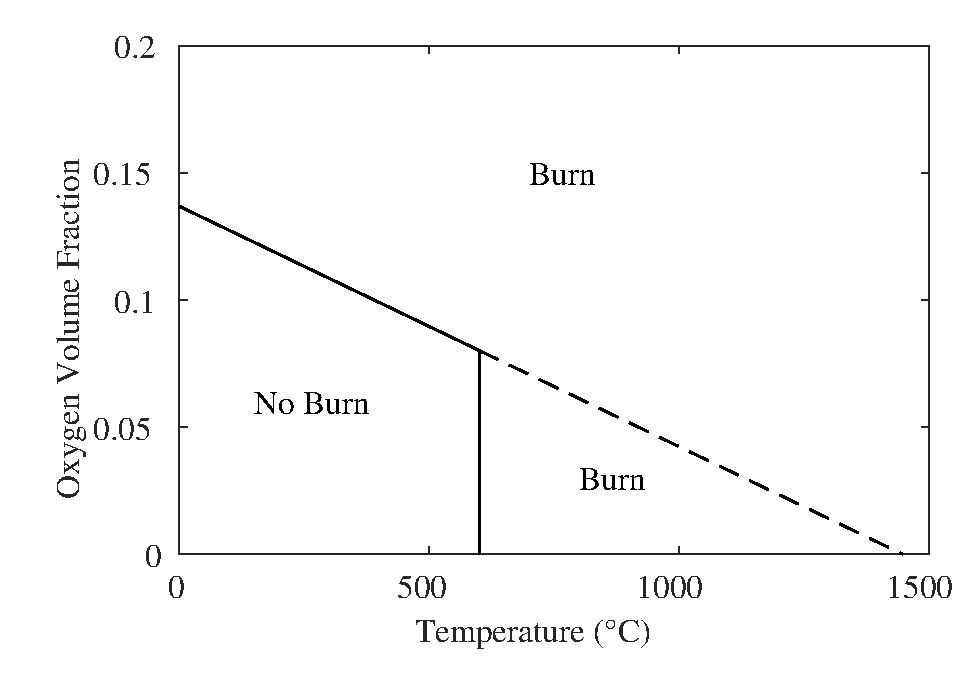
\includegraphics[width=4.5in]{FIGURES/extinction_1_sketch}
\vskip-.2cm
\caption{Extinction criteria for the {\ct 'EXTINCTION 1'} model.}
\label{extinction_1_sketch}
\end{figure}
If $X_{\OTWO,ijk}<X_{\OTWO,\lim}$, local extinction is assumed and $\dot{m}_\alpha'''=0$ and $\dot{q}'''=0$ for that grid cell at that time step. At an ambient temperature of 20~$^\circ$C, the default limiting oxygen volume fraction is 0.135.  This value is consistent with the measurements of Morehart et al.~\cite{Morehart:1991}, who measured the oxygen concentration near self-extinguishing flames. They found that flames self-extinguished at oxygen volume fractions of 12.4~\% to 14.3~\%. Note that their results are expressed as volume, not mass, fractions. Beyler's chapter in the SFPE Handbook references other researchers who measured oxygen concentrations at extinction ranging from 12~\% to 15~\%.

The {\ct 'EXTINCTION 1'} model is intended for relatively coarse fire simulations where the grid cell cannot resolve details of the flame structure or capture flame temperatures. The ``free-burn'' temperature, $T_{\rm fb}$, in Eq.~(\ref{extinction_model}) is needed for simulations in which the characteristic grid cell size, $\dx$, is much larger than 1~cm. In such cases, the combustion occurs within a fraction of the grid cell and its energy cannot raise the cell bulk temperature to the critical value. Its default value is 600~$^\circ$C. Measurements of Pitts~\cite{Pitts:1995}, Bundy~\cite{Bundy:1}, and others, have shown that the upper layer oxygen concentration drops to zero in flashover compartment fire experiments when the temperature increases above approximately 600~$^\circ$C.


\subsection{Extinction Based on Both Fuel and Oxygen}

The second optional extinction model in FDS, referred to as {\ct 'EXTINCTION 2'}, considers both the oxygen and the fuel content of a given grid cell at the start of a time step. If the potential heat release from the reactants cannot raise the temperature of the cell above the empirically determined critical flame temperature, $T_{\rm CFT}$, combustion is suppressed.  Consider the simple reaction $\mbox{Fuel} + \mbox{Air} \rightarrow \mbox{Products}$. The mass fractions of lumped species Fuel, Air, and Products in the mixed portion of the grid cell at the beginning and the end of the reaction part of the time step are $[Z_{\rm F}^0, Z_{\rm A}^0, Z_{\rm P}^0]$ and $[Z_{\rm F}, Z_{\rm A}, Z_{\rm P}]$, respectively. The Products include the products of combustion as well as diluents like argon or water vapor from droplet evaporation. Define a modified form of the equivalence ratio:
\be
   \label{eq:dza}
   \tilde{\phi} \equiv  \min \left( \, 1 \, , \, \frac{s \, Z_{\rm F}^0}{Z_{\rm A}^0} \, \right) = \frac{Z_{\rm A}^0-Z_{\rm A}}{Z_{\rm A}^0}
\ee
where $s$ is the mass stoichiometric coefficient for Air (mass of Air required per mass of Fuel consumed). The extinction criterion assumes that excess fuel acts as a diluent, but excess air and a proportional amount of products do \emph{not}. Hence, a large computational cell that is mostly air with a small amount of fuel is likely to burn, whereas a cell that is mostly fuel with little air will not. To achieve this, a fraction of the total mass of the grid cell equal to $(1-\tilde{\phi}) (Z_{\rm A}^0+Z_{\rm P}^0)$ has been removed from the calculation of the enthalpy. With this amount of mass removed, the extinction criterion is given by:
\begin{equation}
\label{eq:extinction}
Z_{\rm F}^0 \, h_{\rm F}(T) + \tilde{\phi} \, Z_{\rm A}^0 \, h_{\rm A}(T) + \tilde{\phi} \, Z_{\rm P}^0 \, h_{\rm P}(T) <
Z_{\rm F} \, h_{\rm F}(T_{\rm CFT}) + \left[ Z_{\rm P} - (1-\tilde{\phi}) \, Z_{\rm P}^0 \right] \, h_{\rm P}(T_{\rm CFT})
\end{equation}
where $T$ is the pre-reaction mean cell temperature and $T_{\rm CFT}$ is the critical flame temperature. Note that $h_\alpha(T)$ represents the chemical plus sensible enthalpy; thus, the left-hand-side includes the combustion heat release.  If the inequality, (\ref{eq:extinction}), holds, combustion is suppressed---the combustion heat release is not sufficient to raise the product mixture above its critical flame temperature. Notice that the right-hand side of the inequality contains no air because all excess air has been removed from consideration. In other words, for an infinitely fast reaction, $Z_{\rm A}-(1-\tilde{\phi}) Z_{\rm A}^0 \equiv 0$.

This extinction model can be applied to multiple reaction schemes. The critical flame temperature criterion is applied to the entire reaction. In other words, the individual reactions are allowed to occur, and the enthalpy inequality (\ref{eq:extinction}) is applied to the initial and final species mass fractions. If insufficient energy has been released, all reactions are suppressed and the species mass fractions are returned to their original values at the start of the time step.


\subsection{Auto-Ignition Temperature}

As a convenience to users, FDS is designed so that there is no need to create an ignition source to initiate combustion---fuel and air burn on contact until the combustion becomes unviable as discussed above. However, in certain fire scenarios this assumption leads to spurious burning of fuel gas at the boundary of an oxygen-starved compartment. To prevent this, it is possible to turn off the assumption of piloted ignition by way of an auto-ignition temperature. If the cell temperature is below the user-specified auto-ignition temperature (AIT) for all fuels in the cell, combustion is suppressed. The auto-ignition temperature for each fuel is zero by default; thus, the user does not need to specify an ignition source when using the default combustion model because fuel and oxygen burn on contact.

\include{Radiation_Chapter}
\include{Solid_Chapter}
% !TEX root = FDS_Technical_Reference_Guide.tex

\typeout{new file: Particle_Chapter.tex}

\chapter{Lagrangian Particles}
\label{chapter:lagrangian_particles}

Lagrangian particles are used to represent a wide variety of objects that cannot be resolved on
the numerical grid. Liquid droplets are the most common example. This chapter outlines the treatment of the transport, size
distribution, and mass, momentum and energy transfer to and from Lagrangian particles.  The formulation presented here closely follows the dispersed discrete-element formulation presented in \cite{Crowe:1}.

\section{Particle Transport in the Gas Phase}

In the gas phase momentum equation, Eq.~(\ref{momentum}), the force term $\bof_{\rm b}$ represents the momentum transferred from particles to the gas. It is obtained by summing the force transferred from each particle in a grid cell and dividing by the cell volume, $V$:
\be
    {\bof_{\rm b}} = \frac{1}{V} \sum  \left[ \frac{\rho}{2} \, C_{\rm d} \, A_{\rm p,c} \, (\bu_{\rm p}-\bu) |\bu_{\rm p}-\bu| - \frac{\d m_{\rm p}}{\d t} \, (\bu_{\rm p}-\bu) \right] \label{part_force}
\ee
where $C_{\rm d}$ is the drag coefficient, $A_{\rm p,c}$ is the particle cross-sectional area, $r_{\rm p}$ is the particle radius, $\bu_{\rm p}$ is the particle velocity, $m_{\rm p}$ is the particle mass, $\bu$ is the gas velocity, and $\rho$ is the gas density. The subscript ``b'' stands for ``bulk,'' meaning that the particles in the cell represent a bulk mass dragging on the gas.

The particle acceleration is given by
\be
    \frac{\d \bu_{\rm p}}{\d t} = \bg - \ha \frac{\rho\,C_{\rm d} \, A_{\rm p,c}}{m_{\rm p}} \,
    (\bu_{\rm p}-\bu) |\bu_{\rm p}-\bu|
\ee
The particle position, $\bx_{\rm p}$, is determined from the equation
\be
    \frac{\d \bx_{\rm p}}{\d t} = \bu_{\rm p}
\ee
The exact solution procedure of the above model is presented in Appendix~\ref{particle_momentum_transfer}. The drag coefficient (default based on a sphere) is a function of the local Reynolds number that is based on the particle diameter, $D$ ($2 r_{\rm p}$)
\begin{align}
 C_{\rm d} &= \left\{ \begin{array}{ll}
     24/\RE_D                                          & \RE_D < 1    \\[0.1in]
     24\left(0.85+0.15 \, \RE_D^{0.687} \right)/\RE_D  & 1 < \RE_D < 1000 \label{sphere_drag}\\[0.1in]
     0.44                                              & 1000 < \RE_D
     \end{array} \right.  \\[0.2in]
\RE_D &= \frac{\rho \, |\bu_{\rm p}-\bu| \, 2 r_{\rm p}}{\mu(T)} \end{align}
where $\mu(T)$ is the dynamic viscosity of air at temperature $T$~\cite{Crowe:1}\footnote{Note that the 0.85 in the second line of Eq.~(\ref{sphere_drag}) has been inserted to ensure continuity of the functional relationship at $\RE_D=1$.}. For cylindrical particles, the following correlation was derived from data presented by Schlichting~\cite{Schlichting:1}:
\begin{align}
 C_{\rm d} &= \left\{ \begin{array}{ll}
     10/\RE_D^{0.8}                                & \RE_D < 1    \\[0.1in]
     10\left(0.6+0.4 \, \RE_D^{0.8} \right)/\RE_D  & 1 < \RE_D < 1000 \\[0.1in]
     1                                             & 1000 < \RE_D
     \end{array} \right.
\end{align}
Additional corrections are made to account for drag reduction due to the wake effect~\cite{Ramirez:1} and deformation of the droplet~\cite{Loth:1}.


\subsection{Using Lagrangian Particles to Represent Vegetation}

For some applications, it is convenient to use Lagrangian particles to represent stationary vegetation, like grasses or leaves, or airborne vegetation, like burning brands. Typically, these different types of vegetation are grouped into different classes of fuel ``elements'', each of which is represented by a single representative particle in each grid cell. Each representative particle contributes to the bulk force term:
\be
    {\bof_{\rm b}} = \sum_{\rm e} {\bof_{\rm b,e}} \quad ; \quad {\bof_{\rm b,e}} = \frac{\rho}{2} \, C_{\rm d} \, C_{\rm s,e} \,  \beta_{\rm e} \, \sigma_{\rm e} \, (\bu_{\rm p,e}-\bu) |\bu_{\rm p,e}-\bu| + \dot{m}_{\rm p,e}''' \, (\bu_{\rm p,e}-\bu)   \label{part_force_veg}
\ee
The terms with subscript ``e'' refer to a particular class of fuel \underline{e}lements and are determined geometrically or empirically.  The shape factor, $C_{\rm s,e}$, is the ratio of the particle's projected cross sectional area, $A_{\rm p,c}$, to its surface area, $A_{\rm p,s}$. A perfect sphere has a shape factor of $\pi r^2/4 \pi r^2=1/4$, but for actual vegetation, the shape factor is assigned an empirical value that accounts for both shape and orientation. Pine needles, for example, project a different cross sectional area depending on their orientation. The drag coefficient, $C_{\rm d}$, is empirically derived and takes into account both the geometry and shadowing effects of closely packed objects. It is typically expressed as a constant rather than a function of the Reynolds number.  $\beta_{\rm e}$ is the volume fraction; that is, the ratio of the volume occupied by solid mass to the overall volume of the vegetation, sometimes referred to as the {\em packing ratio}. $\sigma_{\rm e}$ is the surface to volume ratio of a single particle. $\dot{m}_{\rm p,e}'''$ is the mass generation rate per unit volume of that particular vegetation element.

A convenient way to describe the geometric properties of vegetation is by specifying the surface to volume ratio, $\sigma_{\rm e}$, the volume (packing) ratio, $\beta_{\rm e}$, and an assumed shape, like a sphere or cylinder. The volume fraction is sometimes expressed as a mass per unit volume, or {\em bulk density}, $m'''=\rho_{\rm e} \, \beta_{\rm e}$, where $\rho_{\rm e}$ is the density of the solid. With this information, and the following relations:
\be
   C_{\rm s,e} = \frac{A_{\rm p,c}}{A_{\rm p,s}} \quad ; \quad  \beta_{\rm e}=\frac{n_{\rm p,e} \, V_{\rm p}}{V} = \frac{m'''}{\rho_{\rm e}} \quad ; \quad \sigma_{\rm e}=\frac{A_{\rm p,s}}{V_{\rm p}}
\ee
we can convert the drag force expression in Eq.~(\ref{part_force_veg}) to its equivalent in Eq.~(\ref{part_force}) where the single particle element is represented as $n_{\rm p,e}$ spheres or cylinders occupying a grid cell volume, $V$. In the model, it is sufficient to have only one weighted particle per grid cell per fuel element to represent all of the actual particles of that vegetation class.

One further simplification of Eq.~(\ref{part_force_veg}) is made by lumping terms into a single {\em frontal area density}
\be
   \kappa_{\rm e} = C_{\rm s,e} \,  \beta_{\rm e} \, \sigma_{\rm e} = \frac{ n_{\rm p,e} \, A_{\rm p,c}}{V} \label{kappa_eq}
\ee
$\kappa_{\rm e}$ can also be thought of as an {\em absorption coefficient} for the purpose of computing thermal radiation absorption. In practice, $\kappa_{\rm e}$ is not determined from Eq.~(\ref{kappa_eq}). Rather, it is obtained by measuring the relative amount of sunlight that penetrates a slab of vegetation of thickness, $L$:
\be
   W = {\rm e}^{-\kappa_{\rm e} L}
\ee
Here, $W$ is the relative area of ``white'' of the shadowgraph formed by sunlight passing through the vegetation. It can also be thought of as the fraction of blue sky one sees when looking through a tree canopy of thickness $L$. It is often referred to as the {\em frontal area index} or {\em frontal area fraction}, not to be confused with the {\em frontal area density}, $\kappa_{\rm e}$.

\subsection{Drag Reduction}
\label{sec:threeway}

Typically, Lagrangian particle models only consider two-way coupling between the gas and particles. This means that each particle interacts with the carrier fluid individually. Momentum lost from a particle is added to the fluid and vice versa. If the spray is dense enough, however, the individual particles influence each other through aerodynamic interactions. These effects cannot be captured by the current Eulerian-Lagrangian model for two reasons. First, the Lagrangian particles occupy no volume in the Eulerian space. Second, the separation lengths would be of sub-grid scale in most practical simulations. The aerodynamic interactions start to have an effect when the average particle spacing is less than 10 diameters~\cite{Prahl:1,Prahl:2}. This corresponds to a particle volume fraction, $\alpha$, of approximately 0.01. Volume fractions as high as this can sometimes be achieved inside water mist sprays. If the spray is even more dense, particle-particle collisions or four-way coupling would need to be considered.

In a configuration where two particles with the same diameter are directly in line, the reduction of the drag force on the second particle can be modeled by the following~\cite{Ramirez:1}:
\be
  C_{\rm d} = C_{\rm d,0} \, \frac{F}{F_0}, \label{eq:dragred}
\ee
where $C_{\rm d,0}$ is the single particle drag coefficient and $F / F_0$ is the hydrodynamic force ratio of the trailing particle to an isolated particle:
\be
  \frac{F}{F_0} = W \left[ 1 + \frac{\RE}{16} \frac{1}{\left( L / D - 1
  / 2 \right)^2} \exp \left( - \frac{\RE}{16} \frac{1}{\left( L / D - 1
  / 2 \right)^{}} \right) \right]. \label{eq:dragredfact}
\ee
where $\RE$ is the single particle Reynolds number, $L$ is the distance between the particles, and $W$ is the non-dimensional, non-disturbed wake velocity at the center of the trailing particle
\be
  W = 1 - \frac{C_{\rm d,0}}{2} \left[ 1 - \exp \left( - \frac{\RE}{16}
  \frac{1}{\left( L / D - 1 / 2 \right)} \right) \right]. \label{eq:Wake-Vel}
\ee
This model assumes that the spheres are traveling directly in-line with each other. As such, this provides an upper bound for the strength of the aerodynamic interactions between two particles of the same size. The average separation distance $L/D$ between particle centers is calculated from the local particle volume fraction and local average particle diameter $\bar{D}$ via
\be
  L/D = \bar{D} \left(\pi/6\alpha \right)^{\frac{1}{3}}.
\ee
This simple approximation assumes that particles are uniformly distributed in each computational cell~\cite{Bhattacharyya2008}.

In reality, the spray is not monodisperse and the separation distance between the interacting particles varies. In the simulation, the drag reduction factor in Eq.~\ref{eq:dragred} is only used when the local droplet volume fraction exceeds \num{1e-5}. The drag reduction model is turned on by default.

As $L/D$ approaches zero, the drag coefficient approaches
\be
  C_{\rm d} = C_{\rm d,0} \left(1 - \frac{C_{\rm d,0}}{2}\right),
\ee
which is 78\% of that for an isolated spherical particle.

An alternative approach to drag reduction was provided by Prahl et al.~\cite{Prahl:1} who studied the interaction between two solid spheres in steady or pulsating flow by detailed numerical simulations. According to their study, the above equation underestimates the drag reduction significantly at small drop-to-drop distances. The inflow pulsations were found to reduce the effect of the drag reduction. At large distances, the two results are similar, the Ram\'{\i}rez-Mu\~{n}oz correlation showing more drag reduction. This is not surprising since the velocity profile of a fully developed axi-symmetric wake behind an axi-symmetric body is used in developing the drag reduction correction in Eqs.~\ref{eq:dragredfact} and \ref{eq:Wake-Vel}. At short distances, the wake is not fully developed and the assumption does not hold.

\newpage
\section{Liquid Droplet Size Distribution}

The cumulative volume distribution for a liquid spray is represented by a combination of log-normal and Rosin-Rammler distributions~\cite{Chan:1}:
\be F_{\rm v}(D) = \left\{ \begin{array}{ll}
   \frac{1}{\sqrt{2\pi}} {\displaystyle \int_0^D} \, \frac{1}{\sigma\, D'} \,
   \exp \left( -\frac{[\ln(D'/D_{\rm v,0.5})]^2}{2\sigma^2} \right) \; \d D'            & (D \le D_{\rm v,0.5}) \\ [0.2in]
   1 - \exp \left( -0.693 \left(\frac{D}{D_{\rm v,0.5}}\right)^\gamma \right)           & (D > D_{\rm v,0.5})
   \end{array} \right.  \ee
where $D_{\rm v,0.5}$ is the median volumetric droplet diameter (i.e., half the mass is carried by droplets with diameters of $D_{\rm v,0.5}$ or less), and $\gamma$ and $\sigma$ are empirical constants equal to approximately 2.4 and 0.48, respectively.\footnote{The Rosin-Rammler and log-normal distributions are smoothly joined if $\sigma=2/(\sqrt{2\pi} \, (\ln\,2) \; \gamma)=1.15/\gamma$ .} Alternatively, the user may specify any form of size distribution using the tabulated input data.

The median droplet diameter is a function of the sprinkler orifice diameter, operating pressure, and geometry. Research at Factory Mutual has yielded a correlation for the median droplet diameter~\cite{Yu:2}
\be
   \frac{D_{\rm v,0.5}}{d} \propto \WE^{-\ot}  \label{dropcor}
\ee
where $d$ is the orifice diameter of the nozzle. The orifice Weber number, the ratio of inertial forces to surface tension forces, is given by
\be
   \WE = \frac{\rho_{\rm p} \, u_{\rm p}^2 \, d}{\sigma}  \label{Weber}
\ee
where $\rho_{\rm p}$ is the liquid density, $u_{\rm p}$ is the discharge velocity, and $\sigma$ is the liquid surface tension (\SI{72.8e-3}{N/m} at \SI{20}{\degreeCelsius} for water).
The discharge velocity can be computed from the mass flow rate, a function of the operating pressure and orifice coefficient known as the K-factor. FM reports that the constant of proportionality in Eq.~(\ref{dropcor}) appears to be independent of flow rate and operating pressure. Three different sprinklers were tested in their study with orifice diameters of \SI{16.3}{\milli m}, \SI{13.5}{\milli m}, and \SI{12.7}{\milli m}, and the constants were approximately 4.3, 2.9, and 2.3, respectively. The strike plates of the two smaller sprinklers were notched, while that of the largest sprinkler was not~\cite{Yu:2}.

In real sprinkler systems, the operating pressure is affected by the number of open nozzles. Typically, the pressure in the piping is high when the first sprinkler activates, and
decreases when more and more sprinkler heads are activated. The pipe pressure has an effect on flow rate, droplet velocity and droplet size distribution. FDS does not predict the variation of pipe pressure; it should be specified by the user. The following dependencies are used to update the droplet boundary conditions for mass flow, droplet speed, and median diameter:
\be
    \dot{m}_{\rm p} \propto p^{1/2} \quad ; \quad u_{\rm p} \propto p^{1/2} \quad ; \quad D_{\rm v,0.5}  \propto  p^{-1/3}
\ee
The droplet diameters are randomly chosen from the given size distribution. The cumulative number fraction (CNF), $F_{\rm n}$, is determined from the cumulative volume fraction, $F_{\rm v}$, as follows
\be
   F_{\rm n}(D) = \int_0^D \frac{F'_{\rm v}(D')}{D'^3} \, \d D'  \left/ \int_0^\infty \, \frac{F'_{\rm v}(D')}{D'^3}
     \, \d D' \right. \quad ; \quad F_{\rm v}' \equiv \frac{\d F_{\rm v}}{\d D}
\ee
Figure~\ref{rosin} displays the Rosin-Rammler/log-normal function and the resulting cumulative number fraction.
\begin{figure}[t]
\begin{center}
\includegraphics[width=4.5in]{SCRIPT_FIGURES/particle_size_distribution}
\caption[Liquid droplet size distribution]{Cumulative Volume Fraction and Cumulative Number
Fraction functions of the droplet size distribution from
a typical industrial-scale sprinkler. The median volumetric diameter, $D_{\rm v,0.5}$, is
1~mm, $\sigma=0.48$ and $\gamma=2.4$.}
\label{rosin}
\end{center}
\end{figure}

The selection of droplet diameters makes use of a stratified sampling technique to ensure that the droplets span the entire range of sizes, even with a relatively small number of droplets. Without the stratification, the tails of the distribution can be poorly represented. The procedure for selecting droplet sizes is as follows:
\begin{enumerate}
\item Suppose that the mass flow rate of the liquid is $\dm$, that the time interval for droplet insertion is $\dt$, and that the number of droplets inserted each time interval is $N$.
\item Divide the droplet diameter range into a number of bins of equal width.
\item Randomly choose $N$ integers, $n_i$, ranging from 1 to the total number of bins.
\item Choose $N$ uniformly distributed real numbers between 0 and 1 and calculate $N$ random droplet diameters:
\be
   D_i = F^{-1}_{\rm n} \Big[ F_{\rm n}(D_{n_i,\min}) + {\cal U}(0,1)\left(F_{\rm n}(D_{n_i,\max})-F_{\rm n}(D_{n_i,\min}) \right) \Big] \label{Ud_strat}
\ee
where ${\cal U}(0,1)$ is a uniformly distributed real number between 0 and 1 and $D_{n_i,\min}$ and $D_{n_i,\max}$ are the minimum and maximum diameters of bin $n_i$.
\item Compute weighting constants for each droplet $C_i = F_{\rm n}(D_{n_i,\max}) - F_{\rm n}(D_{n_i,\min})$.
\item Compute a global weighting constant, C, to maintain the overall mass balance:
    \be \dm \; \dt = C \, \sum_{i=1}^N \; C_i \; \frac{4}{3} \pi \rho_{\rm p}
      \left( \frac{D_i}{2} \right)^3
    \ee
    The mass and heat transferred from each droplet will be multiplied by the weighting factor $C$.
\end{enumerate}

\newpage
\section{Spray Initialization}

The droplets are introduced into the simulation along a spherical surface whose diameter is a specified stand-off distance from the nozzle orifice. It is assumed that the droplets have fully atomized by this stage. The longitude of the initial droplet position, $0\le \theta < 2 \pi$, is randomly chosen from a uniform distribution. The latitude, $0 \le \phi < \pi$, is randomly selected from the following distribution:
\begin{equation}
  f(\phi) = \exp \left[ - \beta \left( \frac{\phi - \phi_{\min}}{\phi_{\max} - \phi_{\min}} \right)^2 \right]
\end{equation}
Note that $\phi=0$ is the south pole of the sphere. The spread parameter, $\beta$, is 5 by default. All the droplets are given the same initial speed in the direction of the surface normal.



\section{Heating and Evaporation of Liquid Droplets}

Liquid droplets can represent either discrete airborne spheres or elements of the thin liquid film that forms on wetted solids. These film ``droplets'' are still individually tracked as Lagrangian particles, but the heat and mass transfer coefficients are different. In the discussion to follow, the term ``droplets'' will be used to describe either form.

Over the course of a time step of the gas phase solver, the droplets in a given grid cell evaporate to form the gas species $\alpha$. The evaporation rate is a function of the liquid equilibrium vapor mass fraction, $Y_{\rm \alpha,\ell}$, the local gas phase vapor mass fraction, $Y_{\rm \alpha,g}$, the (assumed uniform) droplet temperature, $T_{\rm p}$, and the local gas temperature, $T_{\rm g}$. The subscript ``g'' refers to the average of the quantity in the cell occupied by the droplet. The subscript ``p'' refers to the liquid droplet. If the droplet is attached to a solid, $T_{\rm s}$ is the surface temperature. The mass and energy transfer between the gas and the liquid can be described by the following set of equations~\cite{Cheremisinoff:1}
\begin{align}
\frac{\d m_{\rm p}}{\d t} & = - A_{\rm p,s} \, h_{\rm m} \, \rho_{\rm g} \, (Y_{\alpha,\ell} - Y_{\rm \alpha, g}) \label{droplet_mass} \\[0.2in]
\rho_{\rm g} V \frac{d Y_{\rm \alpha, g}}{\d t} & = -\frac{\d m_{\rm p}}{\d t}  \label{droplet_gas_fraction} \\[0.2in]
\frac{\d T_{\rm p}}{\d t} & = \frac{1}{m_{\rm p} \, c_{\rm p}}  \left[ \dq_{\rm r} + A_{\rm p,s} \, h  \, (T_{\rm g}-T_{\rm p}) + \frac{\d m_{\rm p}}{\d t} \; h_{\rm v} \right]  \label{droplet_temp}  \\[0.2in]
\frac{\d T_{\rm g}}{\d t} & = \frac{1}{m_{\rm g} \, c_{\rm g}}  \left[A_{\rm p,s} \, h  \, (T_{\rm p}-T_{\rm g}) + \frac{\d m_{\rm p}}{\d t} \; (h_{\rm v}+h_{\rm l}) \right]  \label{droplet_gas_temp}
\end{align}
The droplet is taken to be a pure liquid of species $\alpha$ (usually, either water or fuel).  Here, $m_{\rm p}$ is the mass of the droplet (or that fraction of the surface film associated with the formerly airborne droplet), $A_{\rm p,s}$ is the surface area of the liquid droplet, $h_{\rm m}$ is the mass transfer coefficient to be discussed below, $\rho_{\rm g}$ is the gas density, $c_{\rm p}$ is the liquid specific heat, $c_{\rm g}$ is the gas specific heat, $h$ is the heat transfer coefficient between the droplet and the gas, $\dq_{\rm r}$ is the rate of radiative heating of the droplet (see Eq.~(\ref{eq:qr})), , $h_{\rm l}$ is the liquid specific enthalpy, and $h_{\rm v}$ is the latent heat of vaporization of the liquid. If the droplet were located on a wall surface there would be a fourth equation for the wall temperature. The vapor mass fraction of the gas, $Y_{\rm \alpha,g}$, is obtained from the gas phase mass transport equations, and the liquid equilibrium vapor mass fraction is obtained from the Clausius-Clapeyron equation
\be X_{\rm \alpha,\ell} = \exp \left[ \frac{h_{\rm v} \, W_{\alpha}}R
      \left( \frac{1}{T_{\rm b}}-\frac{1}{T_{\rm p}} \right) \right]  \quad ; \quad
      Y_{\rm \alpha,\ell} = \frac{X_{\rm \alpha,\ell}}{X_{\rm \alpha,\ell} \, (1-W_{\rm a}/W_{\alpha}) + W_{\rm a}/W_{\alpha}}  \label{clausius_clapeyron} \ee
where $X_{\alpha,\ell}$ is the equilibrium vapor {\em volume} fraction, $W_{\alpha}$ is the molecular weight of the gaseous species $\alpha$, $W_{\rm a}$ is the molecular weight of air, $R$ is the universal gas constant, and $T_{\rm b}$ is the boiling temperature of the liquid at standard atmospheric pressure.

Mass and heat transfer between liquid and gas are described with analogous empirical correlations. The mass transfer coefficient, $h_{\rm m}$, is described by the empirical relationships~\cite{Incropera:1}:
\be
   h_{\rm m} = \frac{\SH \; D_{\rm \ell g}}{L} \quad ; \quad \SH = \left\{ \begin{array}{ll} 2 + 0.6 \; \RE_D^\ha \;           \SC^\ot & \hbox{droplet} \\ [0.1in]
                                                                                 0.037 \;   \RE_L^{\frac{4}{5}} \; \SC^\ot & \hbox{film}     \end{array} \right.
\ee
$\SH$ is the Sherwood number, $D_{\rm \ell g}$ is the binary diffusion coefficient between the liquid vapor and the surrounding gas (usually assumed air), $L$ is a length scale equal to either the droplet diameter or 1~m for a surface film, $\RE_D$ is the Reynolds number of the droplet (based on the diameter, $D$, and the relative air-droplet velocity), $\RE_L$ is the Reynolds number based on the length scale $L$, and $\SC$ is the Schmidt number ($\nu/D_{\rm \ell g}$, assumed 0.6 for all cases).

An analogous relationship exists for the heat transfer coefficient~\cite{Incropera:1}:
\be
   h = \frac{\NU \; k}{L} \quad ; \quad \NU = \left\{ \begin{array}{ll} 2 + 0.6 \; \RE_D^\ha \; \PR^\ot           & \hbox{gas-droplet} \\ [0.1in]
                                                                         0.037 \;   \RE_L^{\frac{4}{5}} \; \PR^\ot & \hbox{gas-film}     \end{array} \right.
\ee
$\NU$ is the Nusselt number, $k$ is the thermal conductivity of the gas, and $\PR$ is the Prandtl number (assumed 0.7 for all cases). In cases where the droplet is actually a portion of the liquid film attached to a solid surface, half of the droplet mass is heated or cooled by the solid surface and half is heated or cooled by the gas.

The exchange of mass and energy between liquid droplets and the surrounding gases (or solid surfaces) is computed droplet by droplet. After the temperature of each droplet is computed, the
appropriate amount of vaporized liquid is added to the given mesh cell, and the cell gas temperature is reduced slightly based on the energy lost to the droplet.

Equation~(\ref{droplet_mass}) through Equation~(\ref{droplet_gas_temp}) are solved semi-implicitly over the course of a gas phase time step as follows. The equilibrium vapor mass fraction, $Y_{\rm \alpha,\ell}^n$, is computed using $T_{\rm p}^n$ via Eq.~(\ref{clausius_clapeyron}), and its value at the next time step is approximated via
\be
Y_{\rm \alpha,\ell}^{n+1} \approx Y_{\rm \alpha,\ell}^n + \left( \frac{\d Y_{\rm \alpha,\ell}}{\d T_{\rm p}} \right)^n \; \Big( T_{\rm p}^{n+1}-T_{\rm p}^n \Big)
\ee
where the derivative of $Y_{\rm \alpha,\ell}$ with respect to temperature is obtained via the chain rule:
\be
\frac{\d Y_{\rm \alpha,\ell}}{\d T_{\rm p}} = \frac{\d Y_{\rm \alpha,\ell}}{\d X_{\rm \alpha,\ell}} \, \frac{\d X_{\rm \alpha,\ell}}{\d T_{\rm p}}  = \frac{W_{\rm a}/W_{\alpha}}{ (X_{\rm \alpha,\ell} (1-W_{\rm a}/W_{\alpha}) + W_{\rm a}/W_{\alpha})^2 } \;
\frac{h_{\rm v} W_{\alpha}}{R \, T_{\rm p}^2} \, \exp \left[ \frac{h_{\rm v} \, W_{\alpha}}R \left( \frac{1}{T_{\rm b}}-\frac{1}{T_{\rm p}} \right) \right]
\ee

Equation~(\ref{droplet_mass}) and Equation~(\ref{droplet_gas_fraction}) are combined with the above result to yield:
\be
   \frac{\d m_{\rm p}}{\d t} = - \frac{A h_{\rm m} \rho_{\rm g}}{2} \frac{2 Y_{\rm \alpha,\ell}^n + \frac{\d Y_{\rm \alpha,\ell}}{\d T_{\rm p}} \Big( T_{\rm p}^{n+1}-T_{\rm p}^n \Big)-2 Y_{\rm \alpha, g}^n} {1+\frac{\Delta t^n A h_{\rm m}}{2 V}} \label{droplet_mass_2}
\ee

This can then be substituted into Equation~(\ref{droplet_temp}) and Equation~(\ref{droplet_gas_temp}) to yield a pair of linear equations for the droplet and gas temperature. If a wall is present, then there will be a third equation for the wall temperature. Once the new temperatures are known, the new droplet temperature can be used in Equation~(\ref{droplet_mass_2}) to determine the amount of evaporated liquid.


\subsection{Filtered Volumetric Source Terms}

The filtered volumetric source terms for mass and energy---which are required in the mass transport equation, Eq.~(\ref{species}), and the divergence expression, Eq.~(\ref{eqn_simplediv1})---are obtained by summation of the individual particle source contributions with a given cell divided by the LES time step, $\delta t_{\si{LES}}$, and the local cell volume, $V_{\si{c}}$. The bulk mass and energy source terms are, respectively,
\begin{equation}
\label{eq:bulk_source}
\dot{m}_{{\rm b},\alpha}^{\ppp} = - \frac{ \sum_p \sum_n \delta m_{\si{p}}^n }{\delta t_{\si{LES}} V_{\si{c}}} \quad ; \quad
\dot{q}_{\rm b}^{\ppp} = - \frac{ \sum_p \sum_n \delta q_{\si{p}}^n }{\delta t_{\si{LES}} V_{\si{c}}} \,\mbox{.}
\end{equation}
where $n$ represents the sub-time step in the integration of the droplet mass and energy equations.  The summation over $p$ is over all the particles within the cell.

\subsection{Lagrangian Contribution to the Velocity Divergence}

In practice, the filtered mass and energy source term contributions to the velocity divergence constraint are collected in a single term denoted {\ct D\_SOURCE} within the code,
\begin{equation}
D_{\si{\tiny SOURCE}} = \frac{1}{\rho} \sum_\alpha \frac{\overline{W}}{W_\alpha} \, \dot{m}_{{\rm b},\alpha}^{\ppp} + \frac{1}{\rho c_p T} \left( \dot{q}_{\rm b}^{\ppp} - \sum_\alpha \dot{m}_{{\rm b},\alpha}^{\ppp} \, \int_{T_{\rm b}}^T c_{p,\alpha} \d T'  \right)
\end{equation}
which is embedded in Eq.~(\ref{eqn_fdsD1}).

\section{Fire Suppression by Water}

The previous sections describe heat transfer from a liquid droplet to a gas, a solid, or both. Although there is some
uncertainty in the values of the respective heat transfer coefficients,
the fundamental physics are fairly well understood. However, when
the droplets encounter burning surfaces,
simple heat transfer correlations become more difficult to apply.
The reason for this is that the water is not only cooling the surface
and the surrounding gas, but it is also changing the pyrolysis rate
of the fuel. If the surface of the fuel is planar, it is possible
to characterize the decrease in the pyrolysis rate as a function of
the decrease in the total heat feedback to the surface. Unfortunately,
most fuels of interest in fire applications are multi-component solids
with complex geometry at scales unresolvable by the computational grid.

\subsection{Droplet Transport on a Surface}

When a liquid droplet hits a solid horizontal surface, it is assigned a
random horizontal direction and moves at a fixed velocity until it
reaches the edge, at which point it drops straight down at the same
fixed velocity. This ``dripping'' velocity has been measured for water to be on
the order of 0.5~m/s~\cite{Hamins:1,Hamins:IAFSS2002}.
While attached to a surface, the ``droplet'' is assumed to form a thin film of liquid that
transfers heat to the solid, and heat and mass to
the gas. The film thickness, $\delta$, is given by
\be
   \delta = \max \left( \delta_{\min} , \sum \frac{4}{3} \, \frac{\pi \, r_{\rm p}^3}{A} \right)
\ee
where $A$ is the area of the wall cell to which the droplet is attached. It is assumed that the minimum film thickness, $\delta_{\min}$, is \SI{1e-5}{m}. This prevents a very small amount of liquid from spreading across the entire cell width. It is also assumed that the liquid is opaque with regard to thermal radiation.

\subsection{Reduction of Pyrolysis Rate due to Water}

To date, most of the work in this area has been performed at Factory Mutual. An important paper on the subject is by Yu {\em et al.}~\cite{Yu:1}. The authors consider dozens of rack storage commodity fires of different geometries and water application rates, and characterize the suppression rates in terms of a few global parameters. Their analysis yields an expression for the total heat release rate from a rack storage fire after sprinkler activation
\be
   \dQ = \dQ_0 \; \mathrm{e}^{-k (t-t_0)}  \label{fmexting}
\ee
where $\dQ_0$ is the total heat release rate at the time of application $t_0$, and $k$ is a fuel-dependent constant. This analysis is based on global water flow and burning rates. Equation~(\ref{fmexting}) accounts for both the cooling of non-burning surfaces as well as the decrease in heat release rate of burning surfaces. In the FDS model, the cooling of unburned surfaces and the reduction in the heat release rate are computed locally. Thus, it is awkward to apply a global suppression rule. However, the exponential nature of suppression by water is observed both locally and globally, thus it is assumed that the local heat release rate per unit area can be expressed in the form~\cite{Hamins:1,Hamins:IAFSS2002}
\be
   \dq''(t) = \dq_0''(t) \; \mathrm{e}^{-\int k(t) \, \d t}
\label{nistexting} \ee
where $\dq_0''(t)$ is the burning rate per unit area of the fuel when no water is applied and $k(t)$ is a linear function of the local water mass per unit area, $m_{\rm w}''$, expressed in units of \si{kg/m^2},
\be
   k(t) = a \; m_{\rm w}''(t) \quad   \hbox{s}^{-1}
\ee
Note that $a$ is an empirical constant that is dependent on the material properties of the solid fuel and its geometrical configuration.



\section{Using Lagrangian Particles to Model Complex Objects}
\label{rad_part_absorb}

There are many real objects that participate in a fire that cannot be modeled easily as solid obstructions that conform to the rectilinear mesh. For example, electrical cables, dry brush, tree branches, and so on, are potential fuels that cannot be well-represented as solid cubes, not only because the geometry is wrong, but also because the solid restricts the movement of hot gases through the complex collection of objects.  Additionally objects such as window screens also impose flow restrictions but are typically not resolvable in an engineering calculation. As a potential remedy for the problem, these objects can be modeled as discrete particles that are either spheres, cylinders or small sheets. Each particle can be assigned a surface type in much the same way as is done for solid obstructions that conform to the numerical grid. The particle is assumed to be thermally-thick, but for simplicity the heat conduction within the particle is assumed to be one-dimensional in either a cylindrical, spherical or cartesian coordinate system.

It is assumed that the particles interact with the surrounding gas via an additional source term in the energy conservation equation. For a grid cell with indices $ijk$, the source term is:
\be \label{eq:qr}
   \dq_{{\rm r},ijk}''' \equiv (-\nabla \cdot \dot{\bq}_{\rm r}'')_{ijk} = \sum \kappa_{\rm p} \left( U_{ijk} - 4 \sigma \, T_{\rm p}^4 \right)
\ee
where the summation is over all the particles within the cell. The effective absorption coefficient for a single particle is given by
\be
   \kappa_{\rm p} = \frac{C_{\rm s} \, A}{\dx \, \dy \, \dz}
\ee
where $C_{\rm s}$ is the shape factor (ratio of cross sectional area to surface area) and $A$ is the surface area of the particle and $\dx \, \dy \, \dz$ is the volume of the cell. The net radiative heat flux onto the surface of the particle is
\be
   \dq_{\rm r,p}'' = \epsilon \left( \frac{U_{ijk}}{4} - \sigma T_{\rm p}^4 \right)
\ee


\subsection{Porous Media (Filters, Screens, Metal Meshes, and Similar Materials)}

Air filters, screens, grating, and similar flow obstructions can all be considered
as type of porous media. In general, material forming the porous media will have dimensions will below that of the grid size (e.g. 100 micron diameter filter fibers on a multi-cm grid).  There is, therefore, no easy way to model these materials using solid obstructions. Lagrangian particles can; however, be used to represent both the drag and the mass of these materials. By placing particles in a plane or volume and assigning the particles a porous media drag law, the effects of the porous media can be modeled. The pressure drop over a length $\Delta x$ through porous media is given by \cite{VafaiTien:1981}:
\be
   \frac {\Delta p}{\Delta x} =  \frac{\mu}{K} u + \rho \frac{Y}{\sqrt{K}} \, u^2
\ee
where $K$ is a permeability constant, $Y$ is an inertial constant, $u$ is the velocity normal to the screen, $\rho$ is the density, and $\mu$ is the viscosity of the gas. In the case of a non-isotropic media, the constants $K$ and $Y$ will vary with the flow direction.
The force vector $\bof_{\rm b}$ in Eq.~(\ref{momentum}) represents the momentum transferred from the screen to the gas:
\be
   \bof_{\rm b} = \left( \frac{\mu}{K} + \rho \frac{Y}{\sqrt{K}} |\bu| \right) \bu
\ee

For the special case of screens, gratings, and similar thin porous materials the permeability and inertial constants have been experimentally correlated to screen porosity.  $K$ and $Y$ are functions of the screen porosity (free area/total area), $\phi$:\cite{Bartzanas:1}:
\be
   K = 3.44 \times 10^{-9} \; \phi^{1.6} \; \; \hbox{m}^2 \quad ; \quad Y = 0.043 \, \phi^{2.13}
\ee
For a screen the force vector must account for the actual screen thickness, $l$, being less than that of the grid cell:
\be
   \bof_{\rm b} = l \; \left( \frac{\mu}{K} + \rho \frac{Y}{\sqrt{K}} |\bu| \right) \left( \frac{u}{\dx} , \frac{v}{\dy} , \frac{w}{\dz} \right)
\ee
This force term essentially spreads the pressure drop over the width of a grid cell.


\section{Turbulent Dispersion}

The effect of subgrid-scale turbulent fluid motion on the velocity and position of a Lagrangian particle may be accounted for using a random walk model \cite{Raman:CF}.  The position of a tracer particle obeys the stochastic differential equation
\be
\mbox{d}\mathbf{x}^* = \left[ \tilde{\mathbf{u}} + \frac{1}{\bar{\rho}}\nabla (\bar{\rho}\,D_t) \right] \,\mbox{d}t + \sqrt{2D_t} \,\mbox{d}\mbox{\textbf{W}}
\ee
where $\mathbf{x}^*$ denotes the particle position (an asterisk signifies a particle property), $\tilde{\mathbf{u}}$ is the resolved LES velocity, $D_t$ is the turbulent diffusivity (taken from an eddy viscosity model, for example), and $\mbox{\textbf{W}}$ is an independent Wiener process.  Notice that if no turbulent diffusion exists, the particle follows the resolved flow.  The term added to the resolved velocity accounts for the deterministic mean drift and the random walk term (Wiener process) accounts for the reorientation effect of unresolved turbulent motion.

For those unfamiliar with stochastic differential equations, the Wiener process may be understood numerically as $\mbox{dW}(t) = (\delta t)^{1/2} \, \zeta(t)$ in the limit $\delta t \rightarrow 0$, where $\zeta(t)$ is an independent standardized Gaussian random variable \cite{Pope:2000}.  In FDS, $\zeta(t)$ are generated from a Box-Muller transform \cite{Box-Muller:1958}.

\include{Device_Chapter}
\include{HVAC_Chapter}


\bibliography{../Bibliography/FDS_refs,../Bibliography/FDS_general,../Bibliography/FDS_mathcomp}

\appendix

%\backmatter

%\addtocontents{toc}{\protect\setcounter{tocdepth}{0}}
\include{Appendices}

\end{document}
